\documentclass[11pt,a4paper]{paper}
\usepackage[latin1]{inputenc}
\usepackage{amsmath}
\usepackage{amsfonts}
\usepackage[super,sort&compress,comma]{natbib}
\usepackage{amssymb}
\usepackage{float}
\usepackage{graphicx}
\usepackage{hyperref}
\usepackage[detect-all]{siunitx}
\usepackage{xr}
\externaldocument{preprint}
\usepackage{rotating}
\usepackage[margin=2cm]{geometry}
\renewcommand{\thefigure}{S\arabic{figure}}
\renewcommand{\theequation}{S\arabic{equation}}
\renewcommand{\thesection}{S\arabic{section}}
\renewcommand{\thetable}{S\Roman{table}}
\title{SI for ``Bayesian determination of the effect of a deep eutectic solvent on the structure of lipid monolayers''}
\author{A.~R.~McCluskey,\textit{$^{ab}$}$^{\ddag}$ A.~Sanchez-Fernandez,\textit{$^{ac}$}$^{\ddag\P}$ K.~J.~Edler,\textit{$^{a}$}$^{\ast}$ \\
S.~C.~Parker,\textit{$^{a}$} A.~J.~Jackson,\textit{$^{cd}$} R.~A.~Campbell,\textit{$^{ef}$} and T.~Arnold \textit{$^{abcg}$}$^{\ast}$}

\institution{${a}$~Department of Chemistry, University of Bath, Claverton Down, Bath, \\
BA2 7AY, UK. \\
${b}$~Diamond Light Source, Harwell Campus, Didcot, OX11 0DE, UK. \\
${c}$~European Spallation Source, SE-211 00 Lund, Sweden. \\
${d}$~Department of Physical Chemistry, Lund University, SE-211 00 Lund, Sweden. \\
${e}$~Institut Laue-Langevin, 71 avenue des Martyrs, 38000, Grenoble, France. \\
${f}$~Division of Pharmacy and Optometry, University of Manchester, Manchester, \\
M13 9PT, UK. \\
${g}$~ISIS Neutron and Muon Source, Science and Technology Facilities Council, \\
Rutherford Appleton Laboratory, Harwell Oxford, Didcot OX11 0QX, UK. \\
${\P}$~Present address: Department of Food Technology, Lund University, SE-211 00 \\
Lund, Sweden. \\
$\ddag$~These authors have contributed equally to the work presented within. \\
$\ast$~k.edler@bath.ac.uk; tom.arnold@esss.se}

\date{\today}

\begin{document}

\maketitle

\section{Materials}
Choline chloride (99 \%, Sigma-Aldrich) and glycerol (99 \%, Sigma-Aldrich) d$_9$-choline chloride (99 \%, 98 \% D, CK Isotopes) and d$_8$-glycerol (99 \%, 98 \% D, CK Isotopes)  were purchased and used without further purification. The DES was prepared by mixing the precursors at the appropriate ratio, and heating at \SI{80}{\celsius} until a homogeneous, transparent liquid formed.\cite{Smith2014} The solvent was equilibrated overnight at \SI{40}{\celsius} and subsequently stored under a dry atmosphere. Due to the limited availability of the deuterated precursors, a fully protonated subphase (hDES) and a partially deuterated subphase (hdDES) were prepared and used during the neutron reflectometry (NR) experiment. The partially deuterated subphase was prepared using the following mixtures of precursors: \SI{1}{\mole} of 0.38 mole-fraction of h-choline chloride/0.62 mole-fraction of d-choline chloride; and \SI{2}{\mole} of 0.56 mole-fraction of h-glycerol/0.44 mole-fraction of d-glycerol. The solvent was subsequently prepared following the procedure discussed above.

The water content of the DES was determined before and after each experiment by Karl-Fischer titration (Mettler Toledo DL32 Karl-Fischer Coulometer, Aqualine Electrolyte A, Aqualine Catholyte CG A) in order to ensure water presence was kept to a minimum. Those measurements showed that the water content of the solvent was kept below \SI{0.3}{wt\percent} during all the experimental procedures presented here, which we assume to be negligible and have little impact on the characteristics of the DES.\cite{Hammond2016,Hammond2017}

DPPC (\SI{>99}{\percent}, C$_{16}$ tails), DMPC (\SI{>99}{\percent}, C$_{14}$ tails), and DMPG (\SI{>99}{\percent}, C$_{14}$ tails) were supplied by Avanti Polar Lipids and DLPC (\SI{>99}{\percent}, C$_{12}$ tails) was supplied by Sigma-Aldrich and all were used as received. Deuterated versions of DPPC (d$_{62}$-DPPC, \SI{>99}{\percent}, deuterated tails-only) and DMPC (d$_{54}$-DPPC, \SI{>99}{\percent}, deuterated tails-only) were supplied by Avanti Polar Lipids and used without further purification. These phospholipids were dissolved in chloroform (\SI{0.5}{\milli\gram\per\milli\liter}) at room temperature. PC indicates the molcule contains a phosphocholine head component, where PG contains a phosphoditylglycerol head component, these are shown in Figure 1.

In the XRR experiment, sample preparation was performed in situ using the standard method for the spreading of insoluble monolayers on water: a certain amount of the phospholipid solution was spread onto the liquid surface in order to provide a given surface concentration. After the evaporation of the chloroform, it is assumed that the resulting system is a liquid subphase with a monolayer of phospholipid at the interface. The surface concentration was modified by closing and opening the barriers of a Langmuir trough (Nima Custom model: 20cm x 40cm with a total volume of approximately 450 ml). In order to minimise the volumes used in the NR experiment (to keep the cost of deuterated compounds to a manageable level) it was not possible to use a Langmuir trough. Instead, small Delrin adsorption troughs (5 x 6 cm with a volume of less than 15 ml) were used that did not have controllable barriers. In this case a volume of the lipid-chloroform solution, calculated to give the equivalent surface area per molecule, was spread onto the surface. So, although the surface coverage was nominally the same as used in the X-ray studies, the lack of precise control over the surface pressure meant that it was not appropriate to co-refine XRR and NR contrasts together.

\section{Methods}
XRR measurements were taken on I07 at Diamond Light Source, at \SI{12.5}{\kilo\eV} photon energy using the double-crystal-deflector\cite{Arnold2012} and a Pilatus 100k detector. The reflected intensity was measured in a momentum transfer range from \SIrange{0.018}{0.7}{\AA^{-1}}. The data were normalised with respect to the incident beam and the background was measured from off-specular region-of-interest and subsequently subtracted. Samples were equilibrated for at least one hour and preserved under an argon atmosphere to minimise the adsorption of water by the subphase. XRR data were collected for each of the lipids, DLPC, DMPC, DPPC and DMPG at four surface pressures (DLPC: 20, 25, 30, and \SI{35}{\milli\newton\meter^{-1}}, DMPC: 20, 25, 30, and \SI{40}{\milli\newton\meter^{-1}}, DPPC: 15, 20, 25, and \SI{30}{\milli\newton\meter^{-1}}, DMPG: 15, 20, 25, and \SI{30}{\milli\newton\meter^{-1}}), as measured with an Aluminium Wilhelmy plate; all measurements were conducted at \SI{22}{\celsius} under a Helium atmosphere. The Aluminium Wilhelmy plate was used over a traditional paper plate because the DES was found to wet Aluminium but not paper, and therefore allowed more reproducible surface pressure measurements.
It is noted that the known phase transitions of DMPC and DMPG are 24 and \SI{23}{\celsius} respectively, which is very close to our measurement temperature. For the sake of our assumptions during analysis it is therefore important that we were able to to determine which phase (LE or LC) the molecules are in. This was done directly using Grazing incident X-ray diffraction (see below).

The NR experiments were performed on FIGARO at the Institut Laue-Langevin using the time-of-flight method.\cite{Campbell2011} Measurements at two incident angles of \SI{0.62}{\degree} and \SI{3.8}{\degree} were carried out to provide reduced data with a momentum transfer range from \SIrange{0.005}{0.25}{\AA^{-1}}. Two surface pressures for each system and contrast were measured (DMPC: 20 and \SI{25}{\milli\newton\meter^{-1}}, DPPC: 15 and \SI{20}{\milli\newton\meter^{-1}}). Similar to the X-ray procedure, samples were given enough time to equilibrate (at least two hours), kept under an inert atmosphere, and all measurements were conducted at \SI{22}{\celsius}.

\section{Literature values for head and tail volumes}
The range of volumes used for phospholipid heads and tails are somewhat inconsistent in the literature. There is a general consensus that the volume of the phosphocholine (PC) head is \SIrange{320}{360}{\cubic\angstrom}, while the phosphatidylglycerol (PG) head is \SIrange{289}{291}{\cubic\angstrom} (see Table \ref{tab:water}).
Tail volumes are also quite variable and, as discussed in the main text, the compaction in chain volumes on a phase transition is often not accounted for\cite{Campbell2018}.
We are interested in comparing the volumes of the lipid components on a non-aqueous liquid.
To allow this comparison, Table \ref{tab:water} gives a variety of literature values for the component volumes of the lipids investigated in this work.

\section{Chemically-consistant model}
Our chemically-consistent model is made up of two layers to define the lipid monolayer; the head layer at the interface with the solvent and tail layer at the interface with the air. The head components have a calculated scattering length, $b_h$, (found as a summation of the X-ray or neutron atomic scattering lengths), and a component volume, $V_h$. These head components make up a layer with a given thickness, $d_h$, and roughness, $\sigma_h$, within which some volume fraction of solvent can intercalate, $\phi_h$. The tail components also have a calculated scattering length, $b_t$, roughness, $\sigma_t$, and a component volume, $V_t$. We have defined the thickness of the tail layer, $d_t$, in terms of the maximum (all-trans) length of the carbon tail, $t_t$, and the angle that the chain is tilted by with respect to the interface normal, $\theta_t$,
%
\begin{equation}
\label{equ:tl}
d_t = t_t \cos{\theta_t}.
\end{equation}
%
This was used to impose a chemically-sensible maximum on the thickness of the lipid tail layer, e.g. it cannot be thicker than the maximum extended length of the lipid tail. The scattering length density (SLD) of the tail and head layers used in the Abel\`{e}s model can therefore be found as follows,
%
\begin{equation}
\text{SLD}_i = \frac{b_i}{V_i}(1 - \phi_i) + \text{SLD}_{s}(\phi_i),
\end{equation}
%
where, $\text{SLD}_{s}$ is the scattering length density of the subphase (DES), and $i$ indicates either the tail or head layer; it is assumed that the tail layer contains neither solvent nor air, i.e. $\phi_t = 0$. To ensure that the number density of head components and pairs of tail components is the same, the following constraint was included in the model,\cite{Braun2017}
%
\begin{equation}
\label{equ:phih}
\phi_h =  1 - \bigg(\frac{d_tV_h}{V_td_h}\bigg).
\end{equation}
%
Based on the work of Campbell \emph{et al.},\cite{Campbell2018} a single value for the interfacial roughness was fitted for all of the interfaces, including the subphase (i.e. $\sigma_h$ = $\sigma_t$ = $\sigma_s$), as there is only a single lipid molecule type in each monolayer. Therefore, the capillary wave roughness at the air-DES interface is carried equally through the layers.
As described in the main text, further constraints were applied to the fitting by co-refining the data across different surface pressures and assuming that the tail volume was constant. This is based on our assumption that there is no phase transition in the monolayer over the surface pressures measured. Thus we have assumed that DPPC is in the LC phase, while DMPC, DMPG and DLPC are all in the LE phase at the measurement temperature.

\section{XRR parameters at each surface pressure}
Tables \ref{tab:liptab1}-\ref{tab:liptab3} give the best fit values for the custom model that were fitted to each surface pressure, for each lipid. These values were used for comparison to assess the effect of the choline chloride:glycerol on the lipid.

\section{Neutron reflectometry and SLD profiles}
Figure \ref{fig:neutron} shows the neutron reflectomery and scattering length density profiles for DMPC at \SI{25}{\milli\newton\per\meter} (two contrasts) and DPPC at \SI{15}{\milli\newton\per\meter} (two contrasts).

\section{Grazing incident X-ray diffraction (GIXD)}
\label{sec:gixd}
We have already indicated that the surface pressure was measured using an Aluminium Wilhelmy plate because the standard paper plates did not wet properly. This method did allow us to measure Langmuir isotherms, but these were inconsistent and as such, not a reliable method for determining the phase of the lipid monolayers.
Instead we were able to measure GIXD for DPPC and DMPC over a range of different surface pressures and temperatures and representative data from these measurements are shown in Figure \ref{fig:gixd} for \SI{30}{\milli\newton\per\meter} and \SI{22}{\celsius} (and \SI{7}{\celsius} for DMPC).  Unfortunately, despite our best efforts, the quality of GIXD data obtained was not entirely satisfactory. All of data contains a weak artefact which we believe is due to scattering from the Teflon trough, which is probably due to the relatively low meniscus of the DES (due to its low surface tension compared to water). In addition we cannot see the expected (1,1) peak observed for these lipids on water. It is unclear whether this is because these peaks are absent or too weak to be measured. Nonetheless, Figure \ref{fig:gixd} shows clear diffraction peaks (which we assume to be the (2, 0)) for DPPC at \SI{22}{\celsius} and for DMPC at \SI{7}{\celsius}. These peaks are also visible at lower surface pressures (data not shown). The presence of any diffraction feature indicates the presence of an LC phase at these temperatures. Importantly there is no such peak observed for DMPC at \SI{22}{\celsius} (see \ref{fig:gixd}), indicating that DMPC is in the LE phase at this temperature. The position of the (2,0) peak, approx \SI{1.48}{\AA^{-1}}, is similar to that found under the same conditions in water.\cite{Watkins2009}
We therefore assume that the phase behaviour on the DES is similar to that observed on water and that the phases observed at \SI{30}{\milli\newton\per\meter} are the same at the other surface pressures measured with XRR and NR. While we have no direct evidence, we have extended this assumption to DLPC and DMPG since there is no reason to believe that the phases of these molecules should be different from that observed for DMPC.

\section{Probability distribution functions}
The two-dimensional probability distribution functions (PDFs) for all parameters and all lipids from the X-ray reflectometry models are given in Figures \ref{fig:dlpc2}-\ref{fig:dmpg5}.
The two-dimensional probability distribution functions (PDFs) for all parameters and all lipids from the neutron reflectometry models are given in Figures \ref{fig:dmpcn1}-\ref{fig:dppcn2}.

These incidate the correlations present between the fitted parameters of the chemically-consistant model.
Particularly noteworthy is the positive correlation between the head thickness, $d_h$, and the solvent concentration in the head layer, $\phi_h$, which shows a clear interaction between these two variables.
This can be rationalised as the smoothing of the interface between the head and the solvent, blurring the values of each variable.
Additionally, it is noted that the correlations present are more substantial for the smaller lipid (particularly DLPC), this is due to the reduced structure presented for such a short tailed lipid and the fact that the length of the tail is closer to the value of the surface roughness for DES (\SI{3.3}{\angstrom}\cite{Sanchez-Fernandez2016}).

\section{Tables and Figures}

\begin{sidewaystable}
  \centering
	\caption{\ Lipid component volumes extracted from different literature sources. $V_l$ corresponds to the total lipid volume, MD to molecular dynamics simulation, WAXS to wide-angle X-ray scattering, NB to neutral buoyancy and DVTD to differential vibrating tube densimetry. $^a$ The values for the head component in Kucerka \emph{et al.},\cite{Kucerka2004} were taken from Balgav\'{y} \emph{et al}.\cite{Balgavy2001}}
  \centering
	\label{tab:water}
	\begin{tabular}{l|lll|ll|ll|l|l}
    Lipid & DPPC & & & DMPC & & DLPC & & DMPG & POPG \\
    \hline
    Reference & [\cite{Armen1998}] & [\cite{Sun1994}] & [\cite{Kucerka2004,Balgavy2001}]$^a$ & [\cite{Armen1998}] & [\cite{Kucerka2004,Balgavy2001}]$^a$ & [\cite{Armen1998}] & [\cite{Kucerka2004,Balgavy2001}]$^a$ & [\cite{Pan2012}] & [\cite{Kucerka2012}] \\
    \hline
    $V_l$/\si{\angstrom^3} & $1287.3\pm25.5$ & $1148\pm2$ & $1264.2\pm32.1$ & $1172.5\pm25.1$ & $1155.4\pm30.0$ & $1057.7\pm24.7$ & $1046.6\pm28.0$ & $1011.4$ & $1203$ \\
    $V_t$/\si{\angstrom^3} & $966.4\pm5.4$ & $829\pm4$ & $924.7\pm17.6$ & $851.5\pm5.0$ & $815.9\pm15.5$ & $736.8\pm4.6$ & $707.1\pm13.5$ & $720.4$ & $914$ \\
    $V_h$/\si{\angstrom^3} & $320.9\pm20.1$ & $319\pm6$ & $339.5\pm14.5$ & $320.9\pm20.1$ & $339.5\pm14.5$ & $320.9\pm20.1$ & $339.5\pm14.5$ & $291.0$ & $289$ \\
    Method & MD & WAXS & NB & MD & NB & MD & NB & DVTD & MD \\
    T/\si{\celsius} & 50 & 24 & 30 & 50 & 30 & 50 & 30 & 20 & 25 \\
	\end{tabular}
\end{sidewaystable}

%
\begin{table}[h]
  \centering
	\caption{\ The invariant parameters within the chemically-consistent model.
	$^a$Values obtained from the Tanford formula.\cite{Tanford1980} $^b$Values obtained from Sanchez-Fernandez \emph{et al.}\cite{Sanchez-Fernandez2016}}
	\label{tab:invariant}
	\begin{tabular}{c|c|c|c|c}
		Component & $b_t$/fm & $b_h$/fm & $t_t$/\AA & $\text{SLD}$/$\times10^{-6}$\AA$^{-2}$ \\
		\hline
		X-ray & & & & \\
		DLPC & 5073 & 4674 & 15.5$^a$ & -- \\
		DMPC & 5985 & 4674 & 18.0$^a$ & -- \\
		DPPC & 6897 & 4674 & 20.5$^a$ & -- \\
		DMPG & 5985 & 4731 & 18.0$^a$ & --\\
		Air & -- & -- & -- & 0\\
		DES & -- & -- & -- & 10.8$^b$ \\
		\hline
		Neutron & & & & \\
		d$_{54}$-DMPC & 5329.8 & 602.7 & 18.0$^a$ & -- \\
		d$_{62}$-DPPC & 6129.2 & 602.7 & 20.5$^a$ & -- \\
		h-DES & -- & -- & -- & 0.43$^b$  \\
		hd-DES & -- & -- & -- & 3.15$^b$ \\
	\end{tabular}
\end{table}
%
%
\begin{table}
  \centering
	\caption{\ The best-fit values, and associated 95 \% confidence intervals for the varying parameters in the XRR models, at the highest surface pressure (SP) measured. The values of $d_t$ were found from the values of $\theta_t$ using Eqn. \ref{equ:tl} and the values for $\phi_h$ were obtained from the use of Eqn. \ref{equ:phih}}
	\label{tab:liptab1}
	\begin{tabular}{l|l|l|l|l}
		Lipid & DLPC & DMPC & DPPC & DMPG \\
    SP/mNm$^{-1}$ & 30 & 30 & 25 & 25 \\
		\hline
		$\theta_t$/$^\circ$ & \input{../output/dlpc/angle35.txt} & \input{../output/dmpc/angle40.txt} & \input{../output/dppc/angle30.txt} & \input{../output/dmpg/angle30.txt} \\
		$\sigma_{t,h,s}$/\AA & \input{../output/dlpc/rough35.txt} & \input{../output/dmpc/rough40.txt} & \input{../output/dppc/rough30.txt} & \input{../output/dmpg/rough30.txt} \\
    \hline
    $V_t$/\AA$^3$ & \input{../output/dlpc/vt.txt} & \input{../output/dmpc/vt.txt} & \input{../output/dppc/vt.txt} & \input{../output/dmpg/vt.txt} \\
		$V_h$/\AA$^3$ & \input{../output/dlpc/vh.txt} & \input{../output/dmpc/vh.txt} & \input{../output/dppc/vh.txt} & \input{../output/dmpg/vh.txt} \\
		$d_h$/\AA & \input{../output/dlpc/head.txt} & \input{../output/dmpc/head.txt} & \input{../output/dppc/head.txt} & \input{../output/dmpg/head.txt} \\
    \hline
    $\phi_h$/$\times10^{-2}$ & \input{../output/dlpc/solh35.txt} & \input{../output/dmpc/solh40.txt} & \input{../output/dppc/solh30.txt} & \input{../output/dmpg/solh30.txt} \\
		$d_t$/\AA & \input{../output/dlpc/tail35.txt} & \input{../output/dmpc/tail40.txt} & \input{../output/dppc/tail30.txt} & \input{../output/dmpg/tail30.txt} \\
	\end{tabular}
\end{table}
%
%
\begin{table}
  \centering
	\caption{\ The best-fit values, and associated 95 \% confidence intervals for the varying parameters in the XRR models, at the second highest surface pressure (SP) measured. The values of $d_t$ were found from the values of $\theta_t$ using Eqn. \ref{equ:tl} and the values for $\phi_h$ were obtained from the use of Eqn. \ref{equ:phih}}
	\label{tab:liptab1}
	\begin{tabular}{l|l|l|l|l}
		Lipid & DLPC & DMPC & DPPC & DMPG \\
    SP/mNm$^{-1}$ & 30 & 30 & 25 & 25 \\
		\hline
		$\theta_t$/$^\circ$ & \input{../output/dlpc/angle30.txt} & \input{../output/dmpc/angle30.txt} & \input{../output/dppc/angle25.txt} & \input{../output/dmpg/angle25.txt} \\
		$\sigma_{t,h,s}$/\AA & \input{../output/dlpc/rough30.txt} & \input{../output/dmpc/rough30.txt} & \input{../output/dppc/rough25.txt} & \input{../output/dmpg/rough25.txt} \\
    \hline
    $V_t$/\AA$^3$ & \input{../output/dlpc/vt.txt} & \input{../output/dmpc/vt.txt} & \input{../output/dppc/vt.txt} & \input{../output/dmpg/vt.txt} \\
		$V_h$/\AA$^3$ & \input{../output/dlpc/vh.txt} & \input{../output/dmpc/vh.txt} & \input{../output/dppc/vh.txt} & \input{../output/dmpg/vh.txt} \\
		$d_h$/\AA & \input{../output/dlpc/head.txt} & \input{../output/dmpc/head.txt} & \input{../output/dppc/head.txt} & \input{../output/dmpg/head.txt} \\
    \hline
    $\phi_h$/$\times10^{-2}$ & \input{../output/dlpc/solh30.txt} & \input{../output/dmpc/solh30.txt} & \input{../output/dppc/solh25.txt} & \input{../output/dmpg/solh25.txt} \\
		$d_t$/\AA & \input{../output/dlpc/tail30.txt} & \input{../output/dmpc/tail30.txt} & \input{../output/dppc/tail25.txt} & \input{../output/dmpg/tail25.txt} \\
	\end{tabular}
\end{table}
%
%
\begin{table}
  \centering
	\caption{\ The best-fit values, and associated 95 \% confidence intervals for the varying parameters in the XRR models, at the second lowest surface pressure (SP) measured. The values of $d_t$ were found from the values of $\theta_t$ using Eqn. \ref{equ:tl} and the values for $\phi_h$ were obtained from the use of Eqn. \ref{equ:phih}}
	\label{tab:liptab2}
	\begin{tabular}{l|l|l|l|l}
		Lipid & DLPC & DMPC & DPPC & DMPG \\
    SP/mNm$^{-1}$ & 25 & 25 & 20 & 20 \\
		\hline
		$\theta_t$/$^\circ$ & \input{../output/dlpc/angle25.txt} & \input{../output/dmpc/angle25.txt} & \input{../output/dppc/angle20.txt} & \input{../output/dmpg/angle20.txt} \\
		$\sigma_{t,h,s}$/\AA & \input{../output/dlpc/rough25.txt} & \input{../output/dmpc/rough25.txt} & \input{../output/dppc/rough20.txt} & \input{../output/dmpg/rough20.txt} \\
    \hline
    $V_t$/\AA$^3$ & \input{../output/dlpc/vt.txt} & \input{../output/dmpc/vt.txt} & \input{../output/dppc/vt.txt} & \input{../output/dmpg/vt.txt} \\
		$V_h$/\AA$^3$ & \input{../output/dlpc/vh.txt} & \input{../output/dmpc/vh.txt} & \input{../output/dppc/vh.txt} & \input{../output/dmpg/vh.txt} \\
		$d_h$/\AA & \input{../output/dlpc/head.txt} & \input{../output/dmpc/head.txt} & \input{../output/dppc/head.txt} & \input{../output/dmpg/head.txt} \\
    \hline
    $\phi_h$/$\times10^{-2}$ & \input{../output/dlpc/solh25.txt} & \input{../output/dmpc/solh25.txt} & \input{../output/dppc/solh20.txt} & \input{../output/dmpg/solh20.txt} \\
		$d_t$/\AA & \input{../output/dlpc/tail25.txt} & \input{../output/dmpc/tail25.txt} & \input{../output/dppc/tail20.txt} & \input{../output/dmpg/tail20.txt} \\
	\end{tabular}
\end{table}
%
%
\begin{table}
  \centering
	\caption{\ The best-fit values, and associated 95 \% confidence intervals for the varying parameters in the XRR models, at the lowest surface pressure (SP) measured. The values of $d_t$ were found from the values of $\theta_t$ using Eqn. \ref{equ:tl} and the values for $\phi_h$ were obtained from the use of Eqn. \ref{equ:phih}}
	\label{tab:liptab3}
	\begin{tabular}{l|l|l|l|l}
		Lipid & DLPC & DMPC & DPPC & DMPG \\
    SP/mNm$^{-1}$ & 20 & 20 & 15 & 15 \\
		\hline
		$\theta_t$/$^\circ$ & \input{../output/dlpc/angle20.txt} & \input{../output/dmpc/angle20.txt} & \input{../output/dppc/angle15.txt} & \input{../output/dmpg/angle15.txt} \\
		$\sigma_{t,h,s}$/\AA & \input{../output/dlpc/rough20.txt} & \input{../output/dmpc/rough20.txt} & \input{../output/dppc/rough15.txt} & \input{../output/dmpg/rough15.txt} \\
    \hline
    $V_t$/\AA$^3$ & \input{../output/dlpc/vt.txt} & \input{../output/dmpc/vt.txt} & \input{../output/dppc/vt.txt} & \input{../output/dmpg/vt.txt} \\
		$V_h$/\AA$^3$ & \input{../output/dlpc/vh.txt} & \input{../output/dmpc/vh.txt} & \input{../output/dppc/vh.txt} & \input{../output/dmpg/vh.txt} \\
		$d_h$/\AA & \input{../output/dlpc/head.txt} & \input{../output/dmpc/head.txt} & \input{../output/dppc/head.txt} & \input{../output/dmpg/head.txt} \\
    \hline
    $\phi_h$/$\times10^{-2}$ & \input{../output/dlpc/solh20.txt} & \input{../output/dmpc/solh20.txt} & \input{../output/dppc/solh15.txt} & \input{../output/dmpg/solh15.txt} \\
		$d_t$/\AA & \input{../output/dlpc/tail20.txt} & \input{../output/dmpc/tail20.txt} & \input{../output/dppc/tail15.txt} & \input{../output/dmpg/tail15.txt} \\
	\end{tabular}
\end{table}
%

\begin{figure}[H]
	\centering
	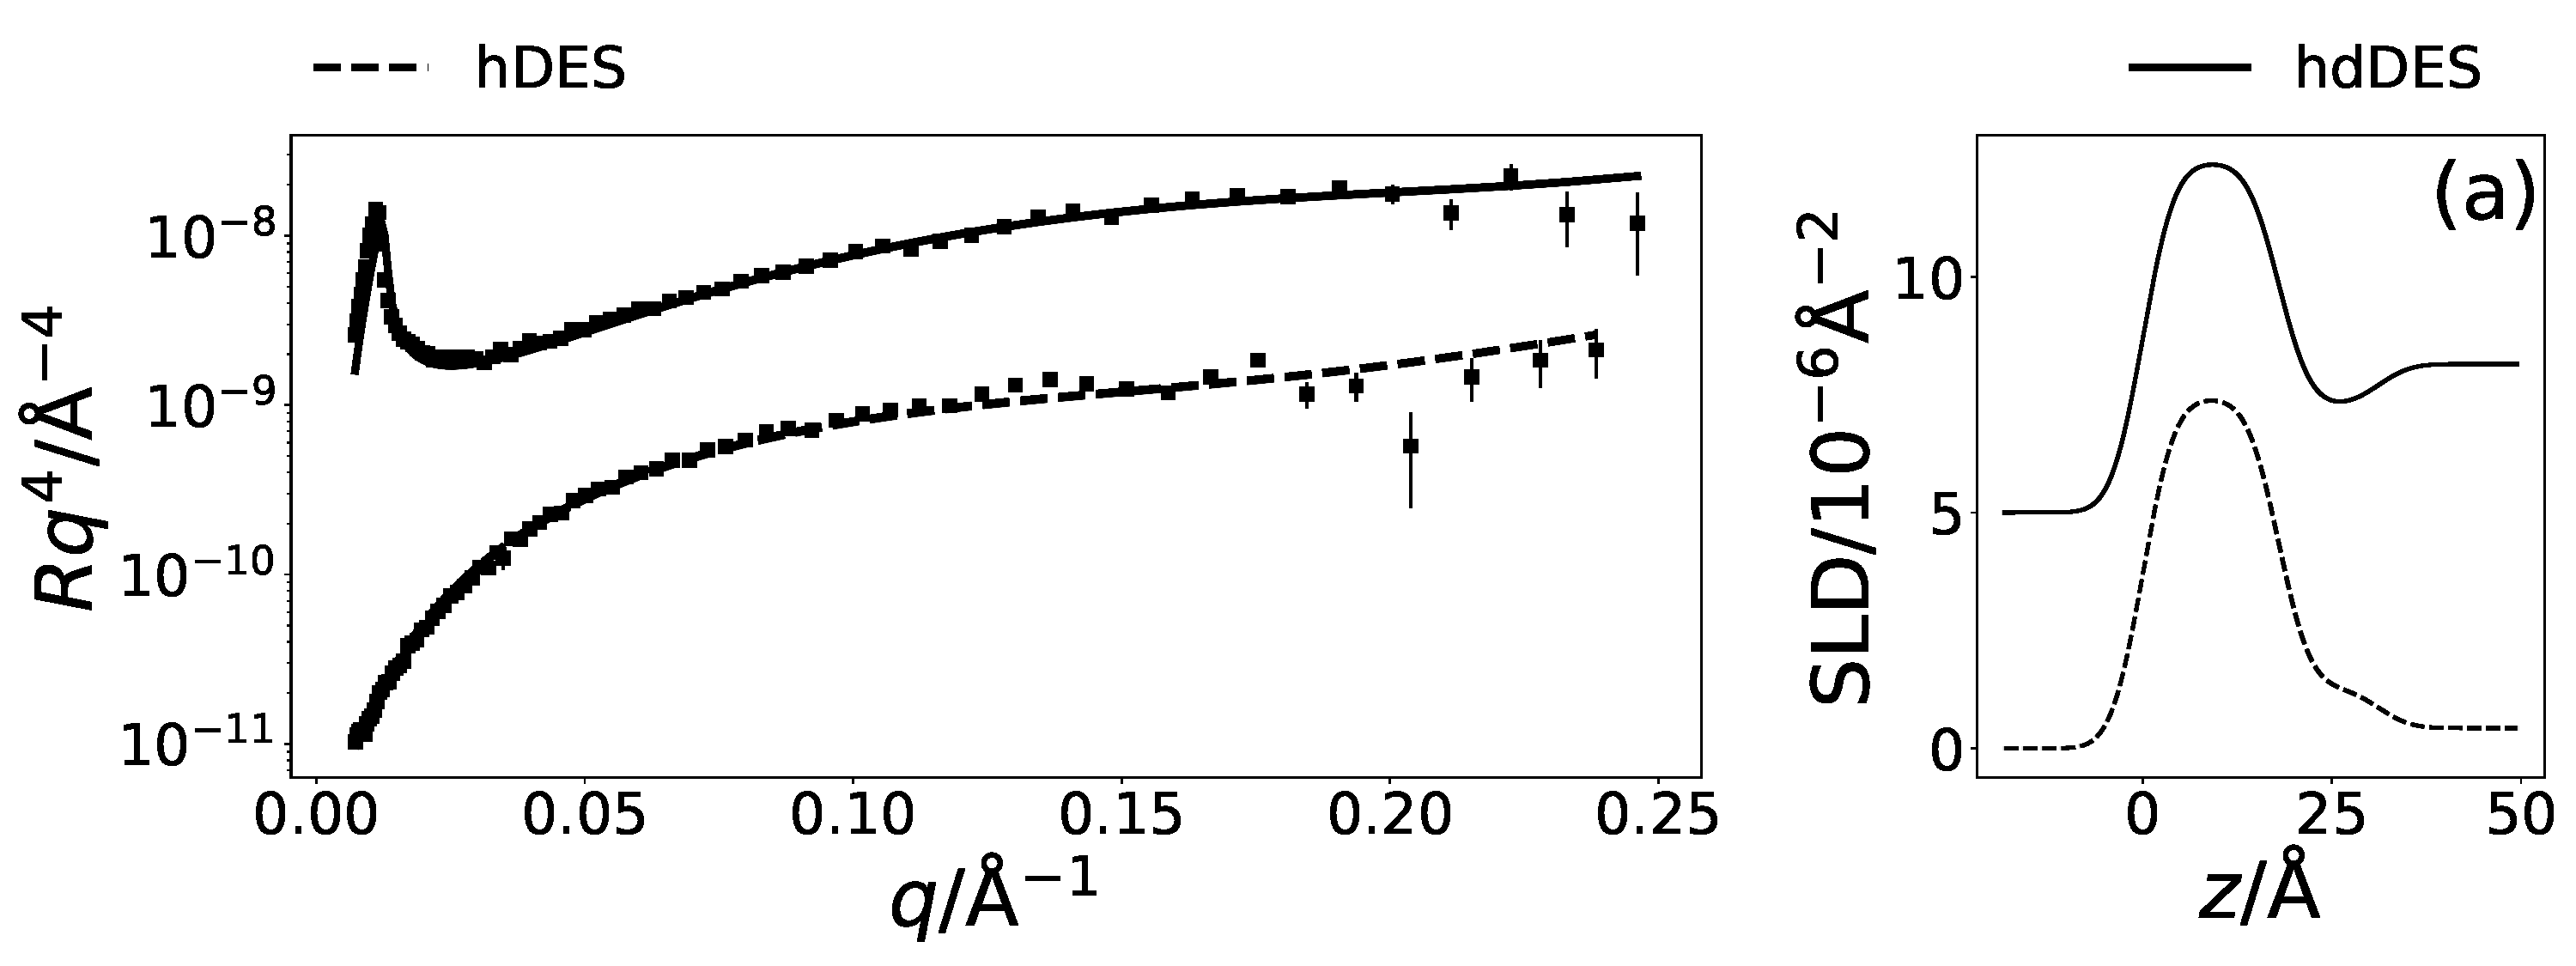
\includegraphics[width=0.9\textwidth]{figures/dmpc_25n_ref_sld}
	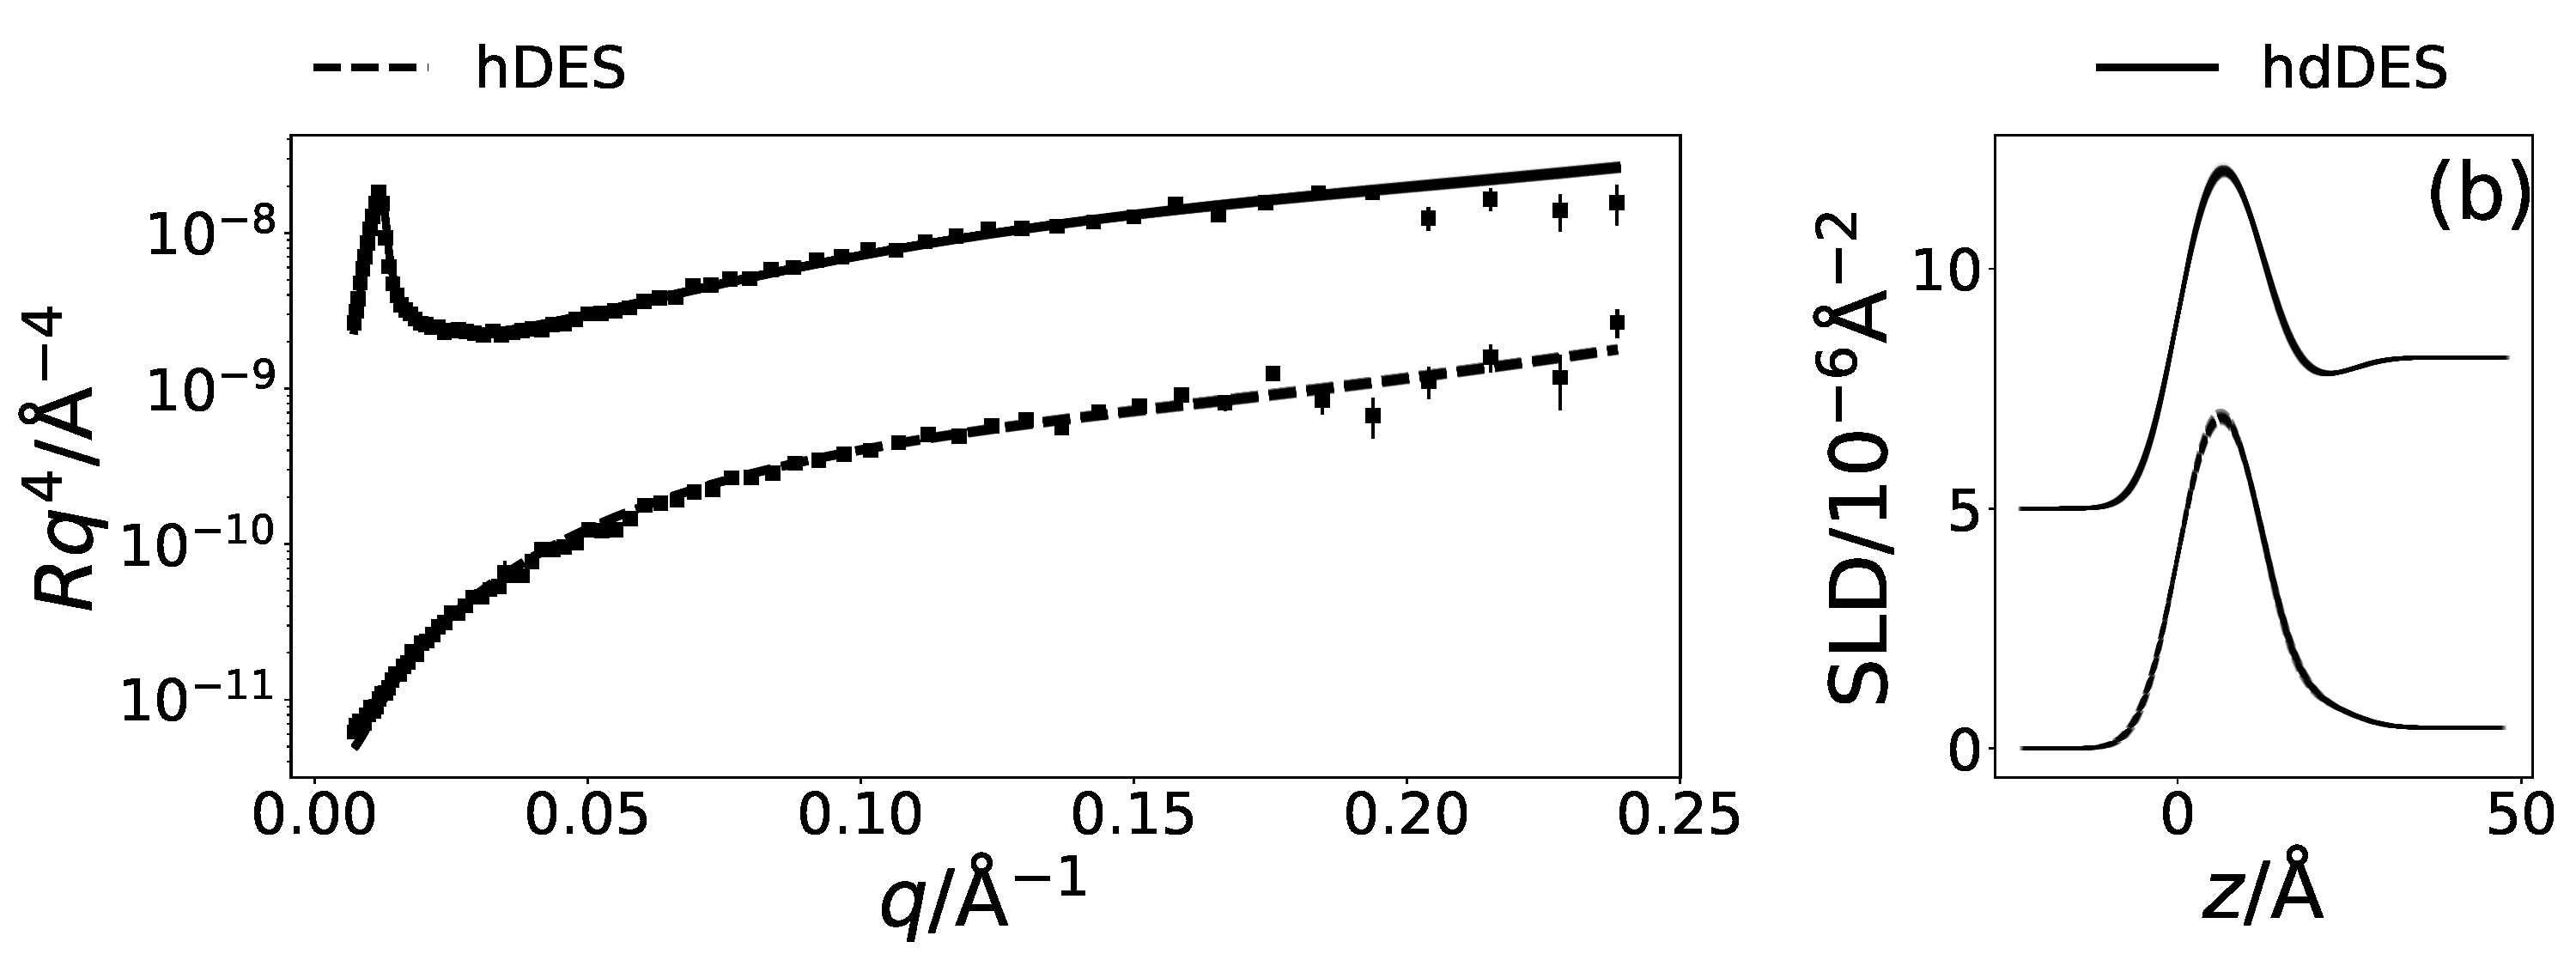
\includegraphics[width=0.9\textwidth]{figures/dppc_15n_ref_sld}
	\caption{The NR and SLD profiles at a surface pressure of (a) 25 mNm$^{-1}$ for two contrasts of DMPC, and (b) 15 mNm$^{-1}$ for two contrasts of DPPC. The NR profiles have been offset in the $y$-axis by an order of magnitude and SLD profiles offset in the $y$-axis by \SI{5e-6}{\per\square\angstrom}, for clarity.}
	\label{fig:neutron}
\end{figure}

\begin{figure}[H]
	\centering
	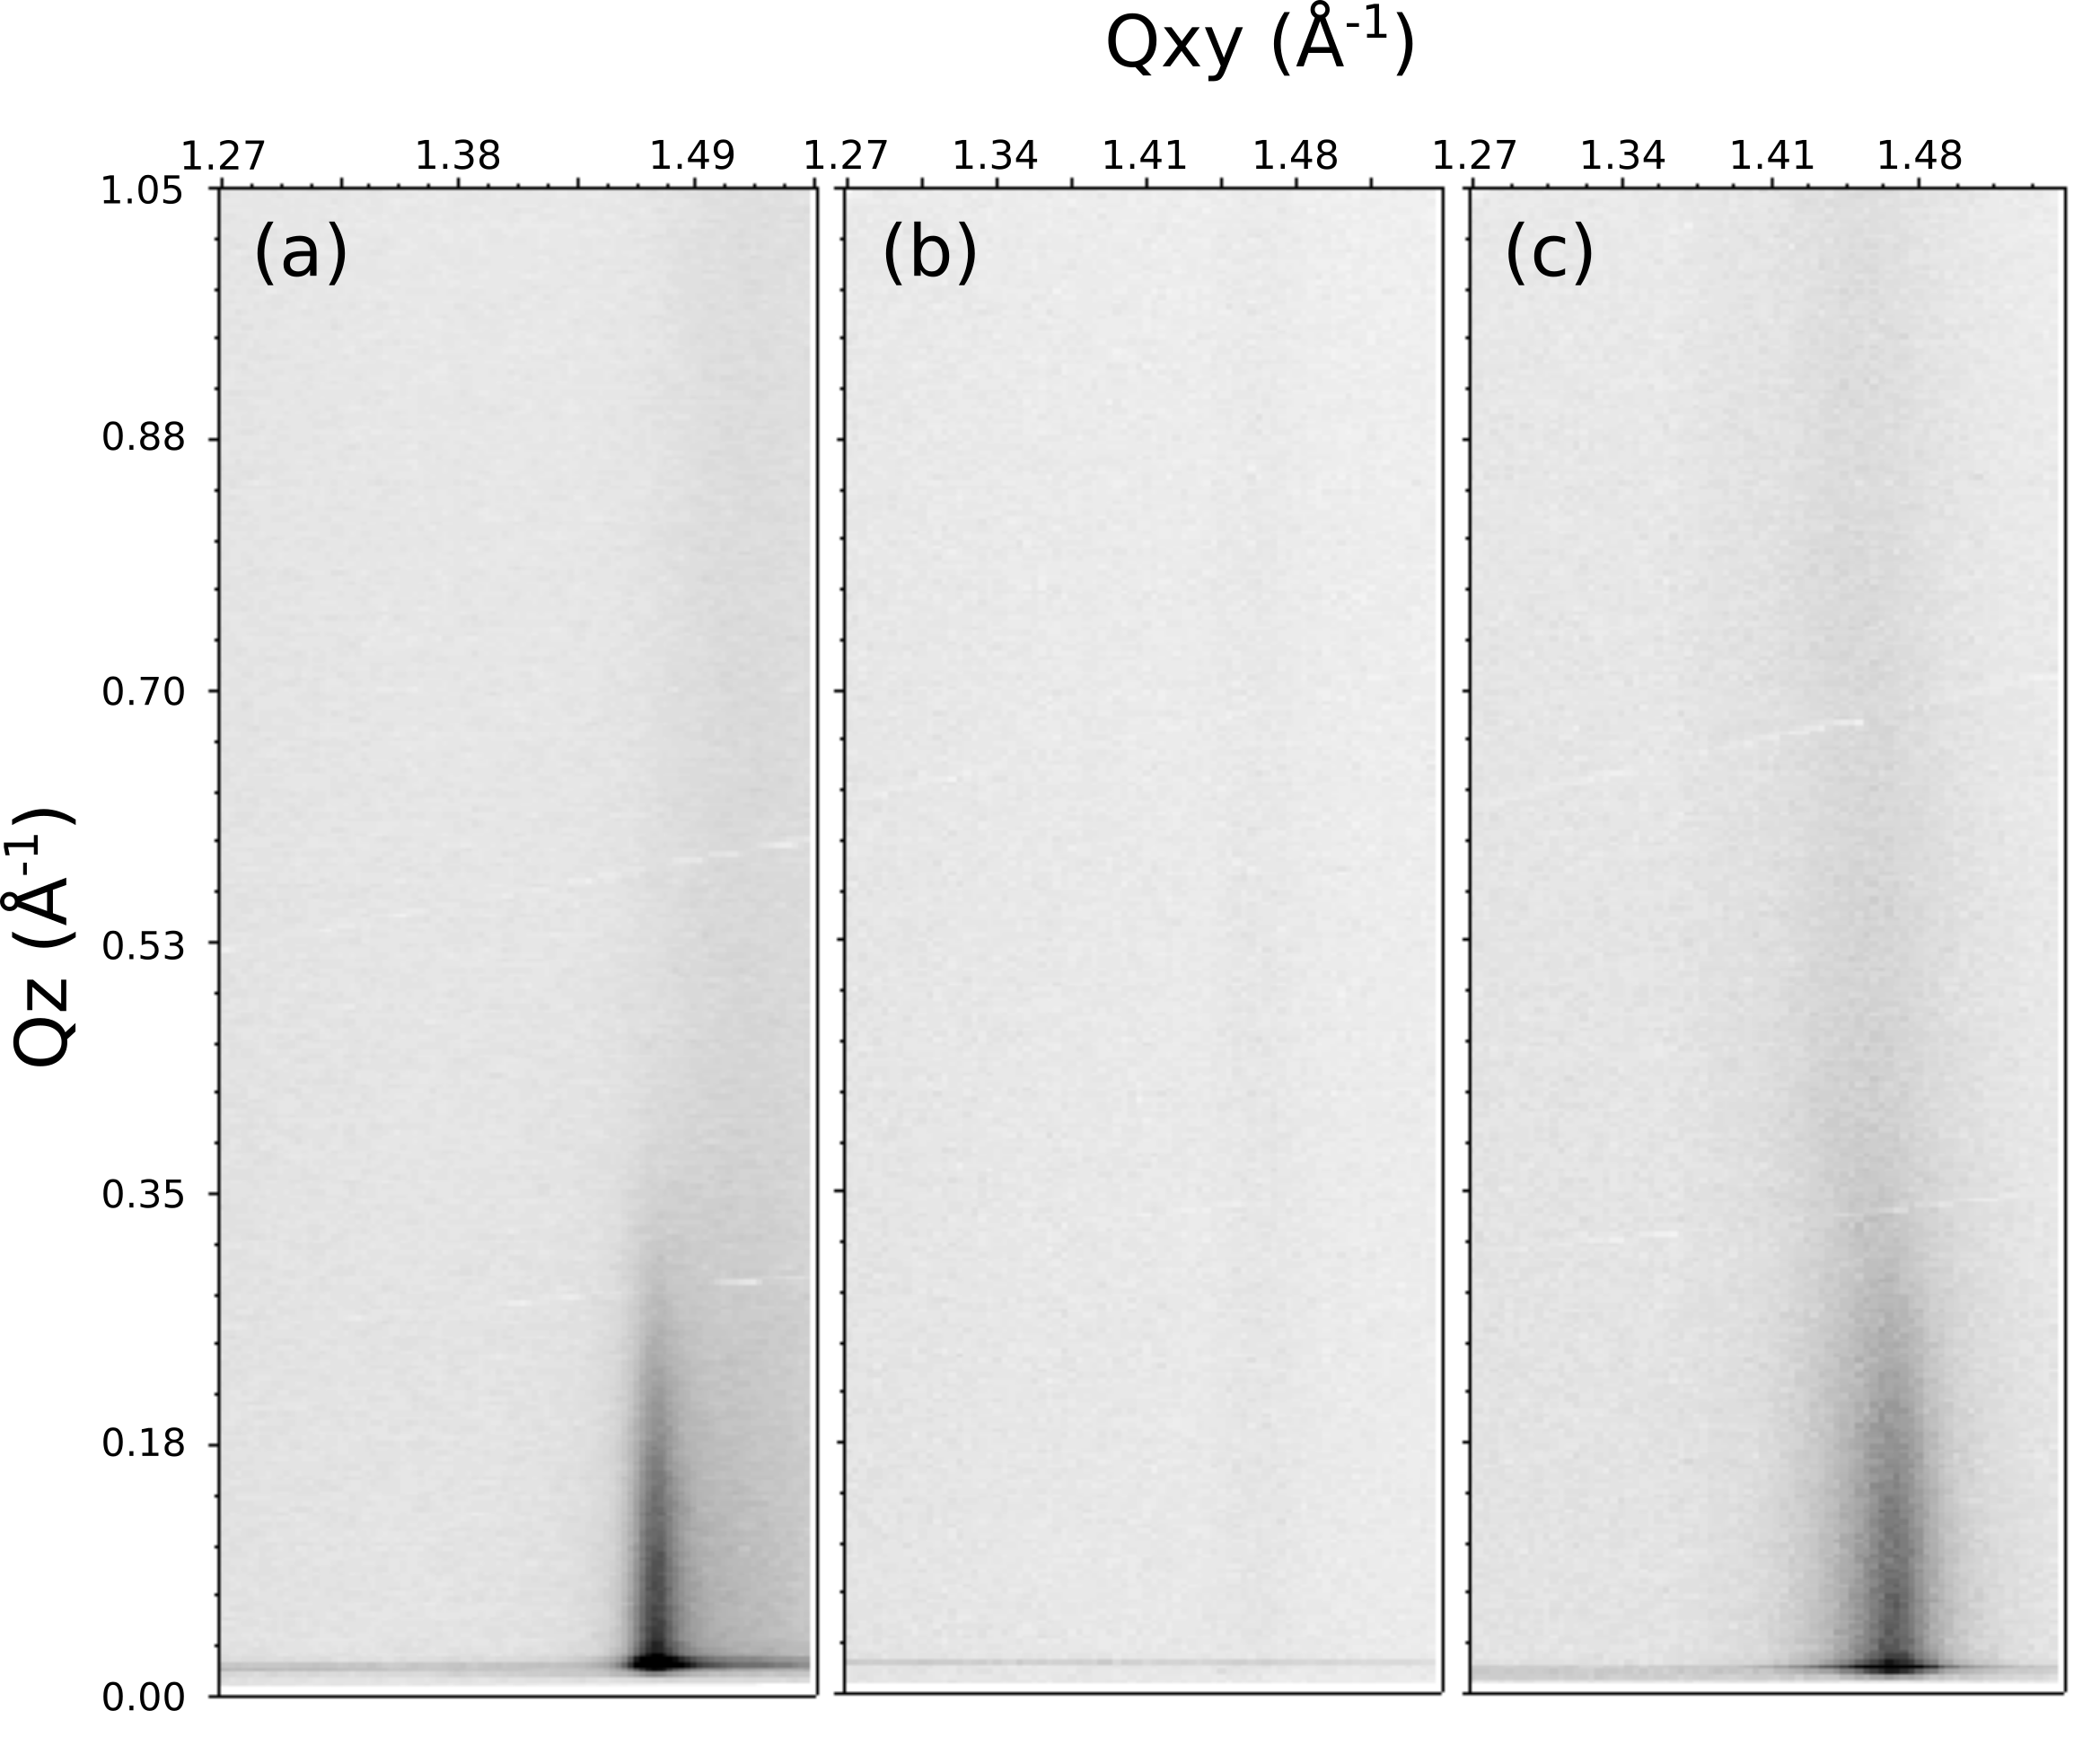
\includegraphics[width=0.50\textwidth]{figures/gixd}
	\caption{The GIXD pattern for (a) DPPC at \SI{30}{\milli\newton\per\meter} at \SI{22}{\celsius}, (b) DMPC at \SI{30}{\milli\newton\per\meter} at \SI{22}{\celsius}, and (c) DMPC at \SI{30}{\milli\newton\per\meter} at \SI{7}{\celsius}.}
	\label{fig:gixd}
\end{figure}

\begin{figure}[H]
	\centering
	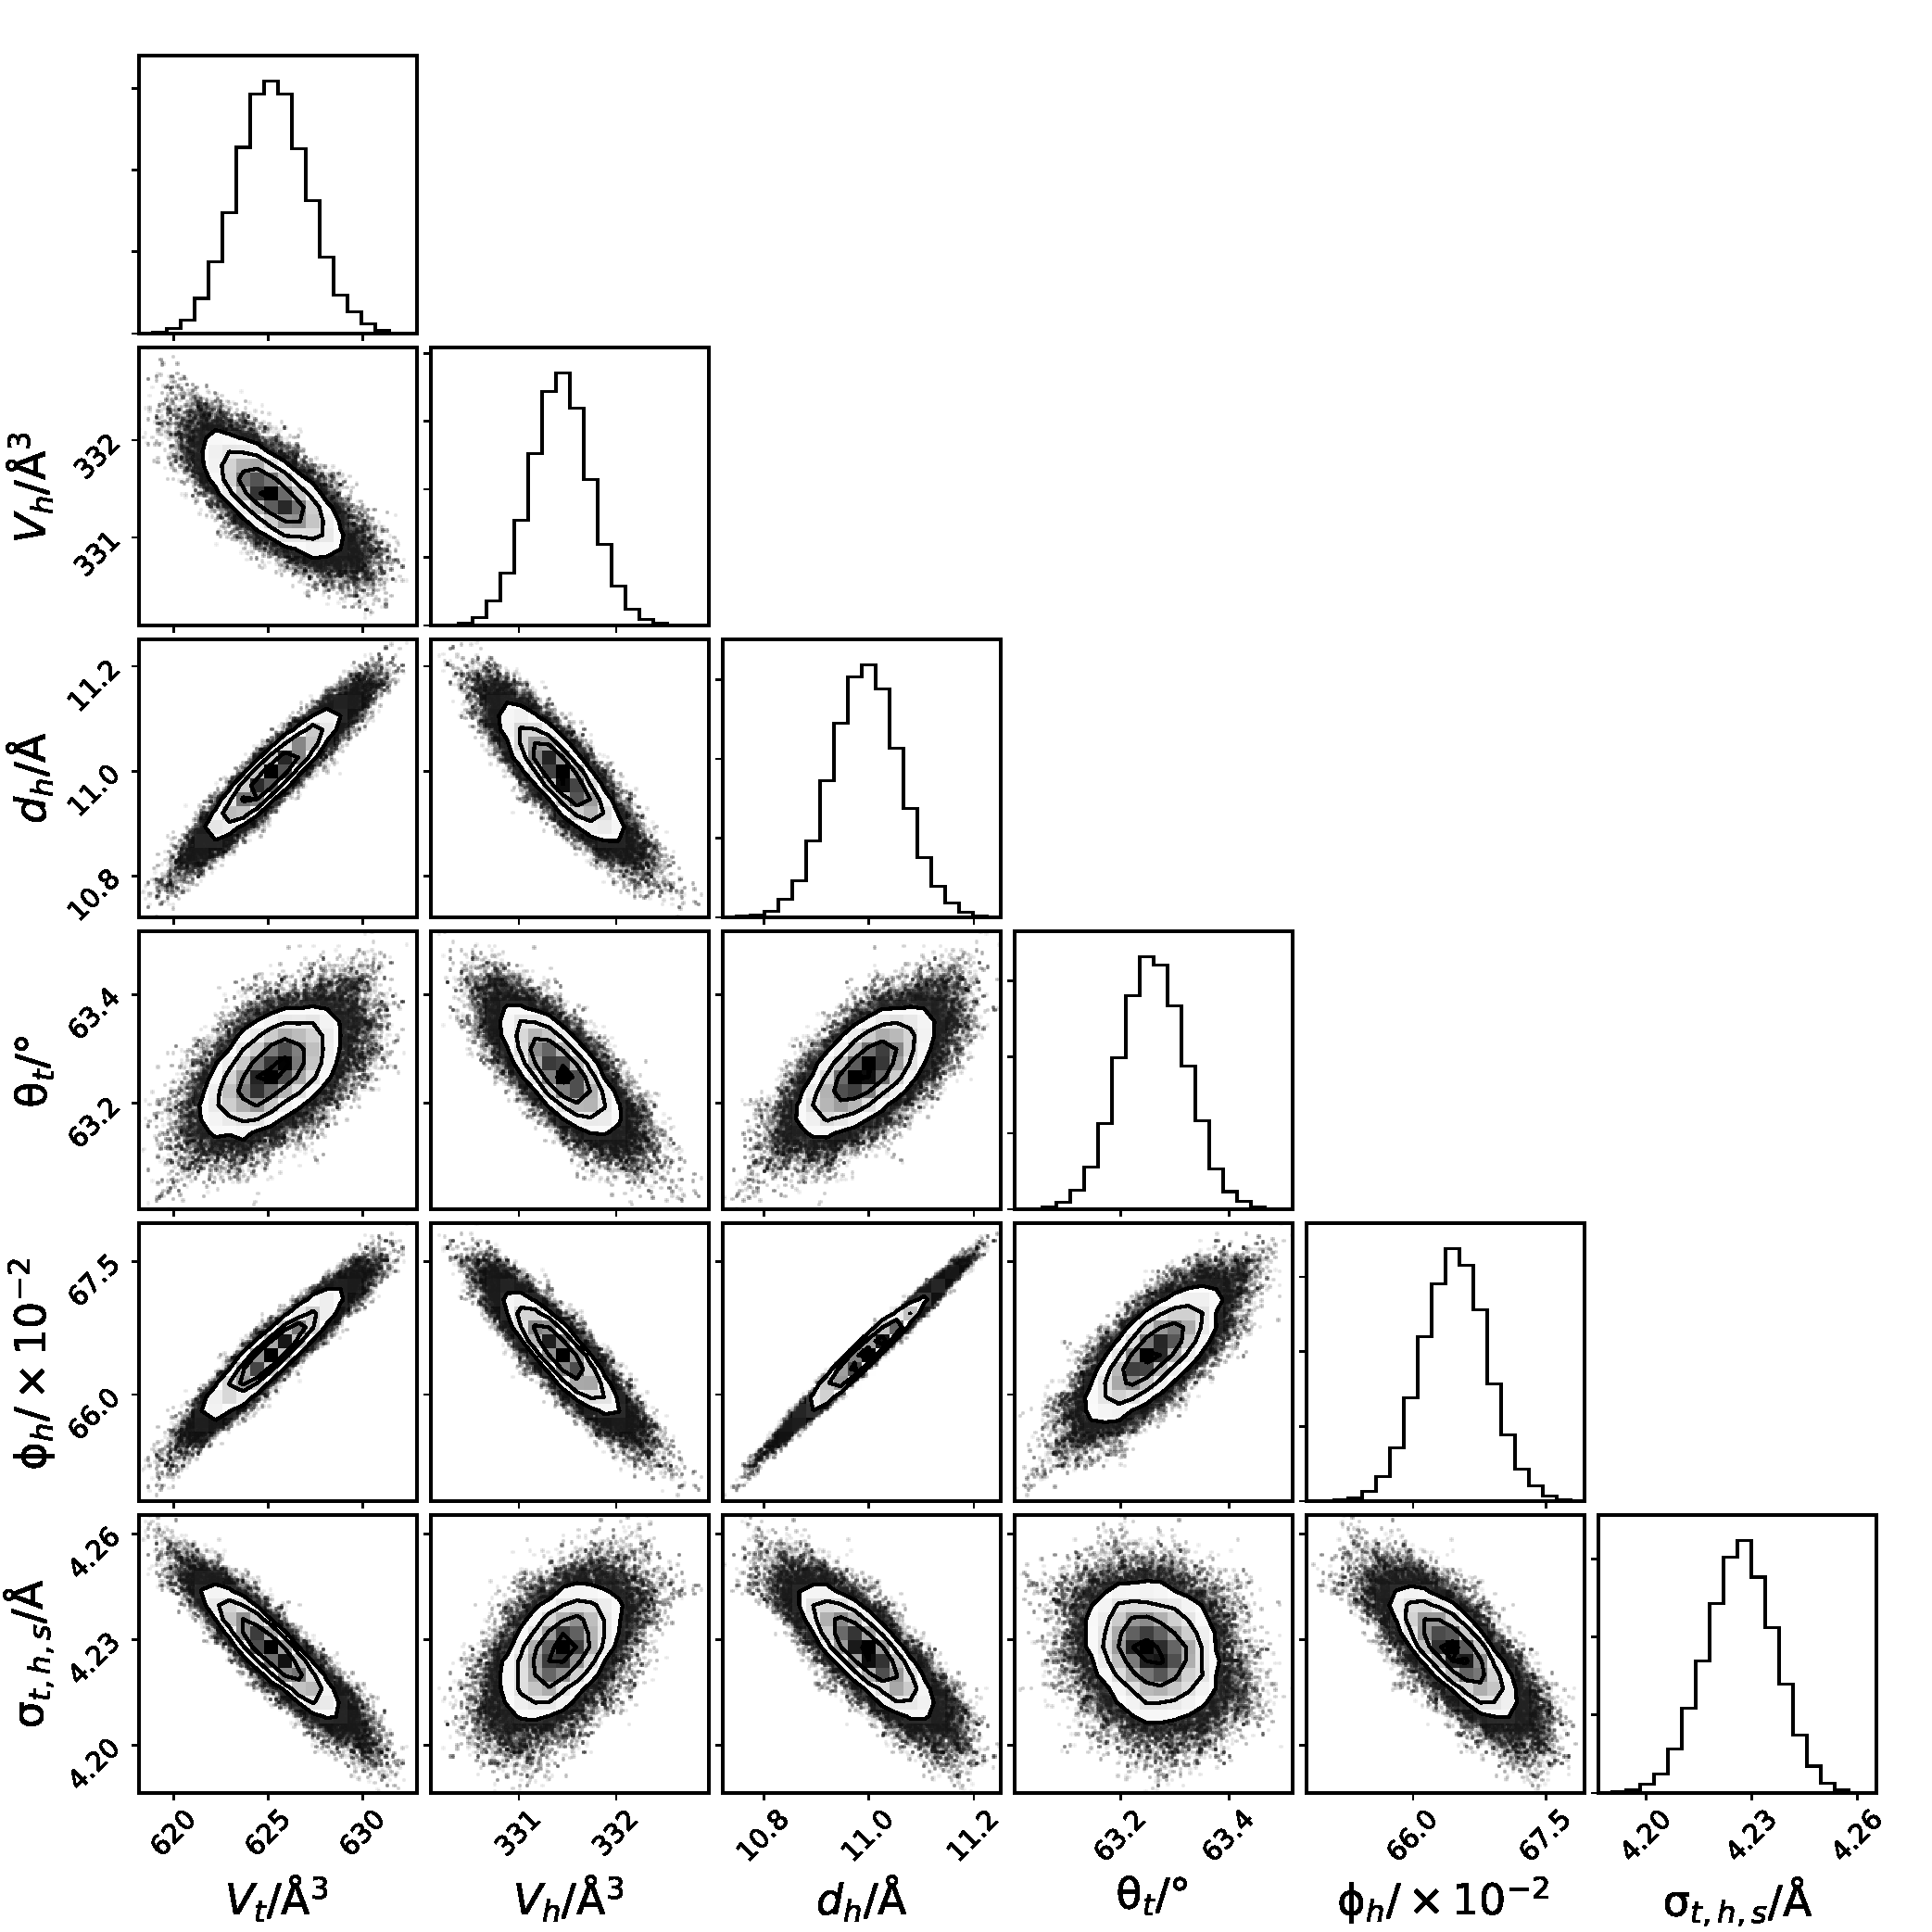
\includegraphics[width=0.50\textwidth]{figures/dlpc1_all_corner}
	\caption{The multi-parameter PDFs for the chemically-relevant model of DLPC X-ray reflectometry data at 20 mNm$^{-1}$.}
	\label{fig:dlpc2}
\end{figure}
\begin{figure}[H]
	\centering
	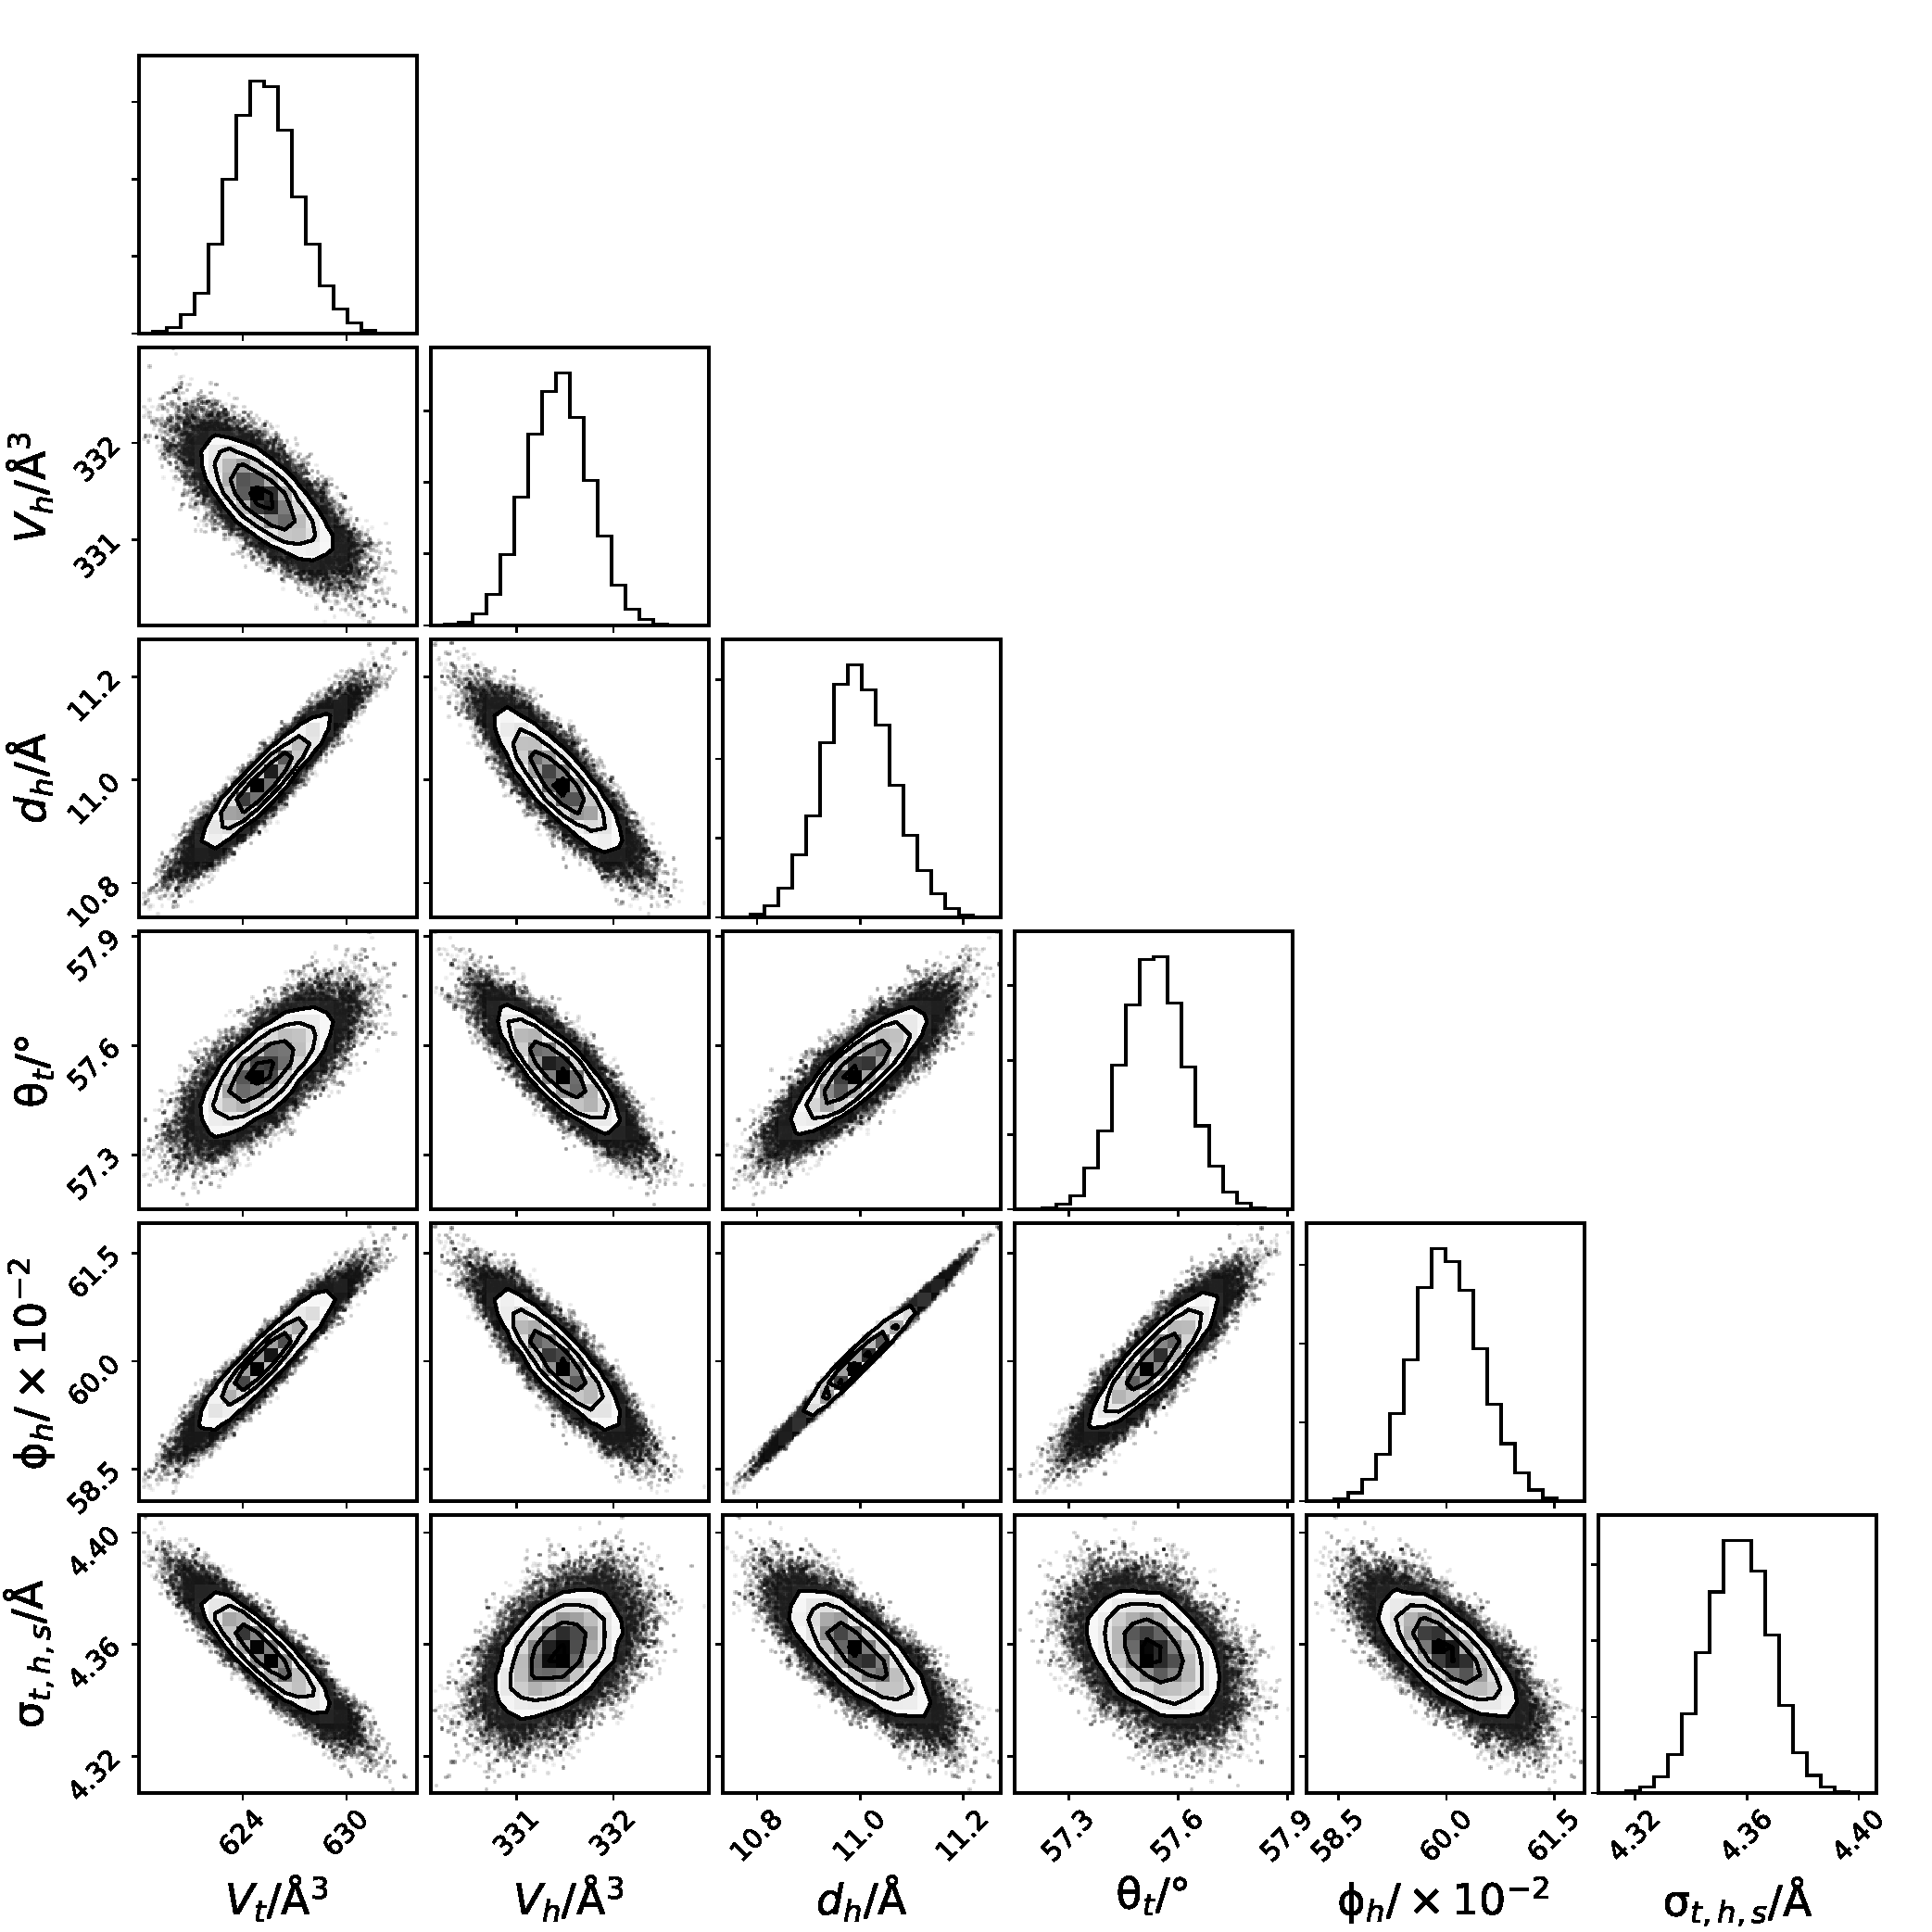
\includegraphics[width=0.50\textwidth]{figures/dlpc2_all_corner}
	\caption{The multi-parameter PDFs for the chemically-relevant model of DLPC X-ray reflectometry data at 25 mNm$^{-1}$.}
	\label{fig:dlpc3}
\end{figure}
\begin{figure}[H]
	\centering
	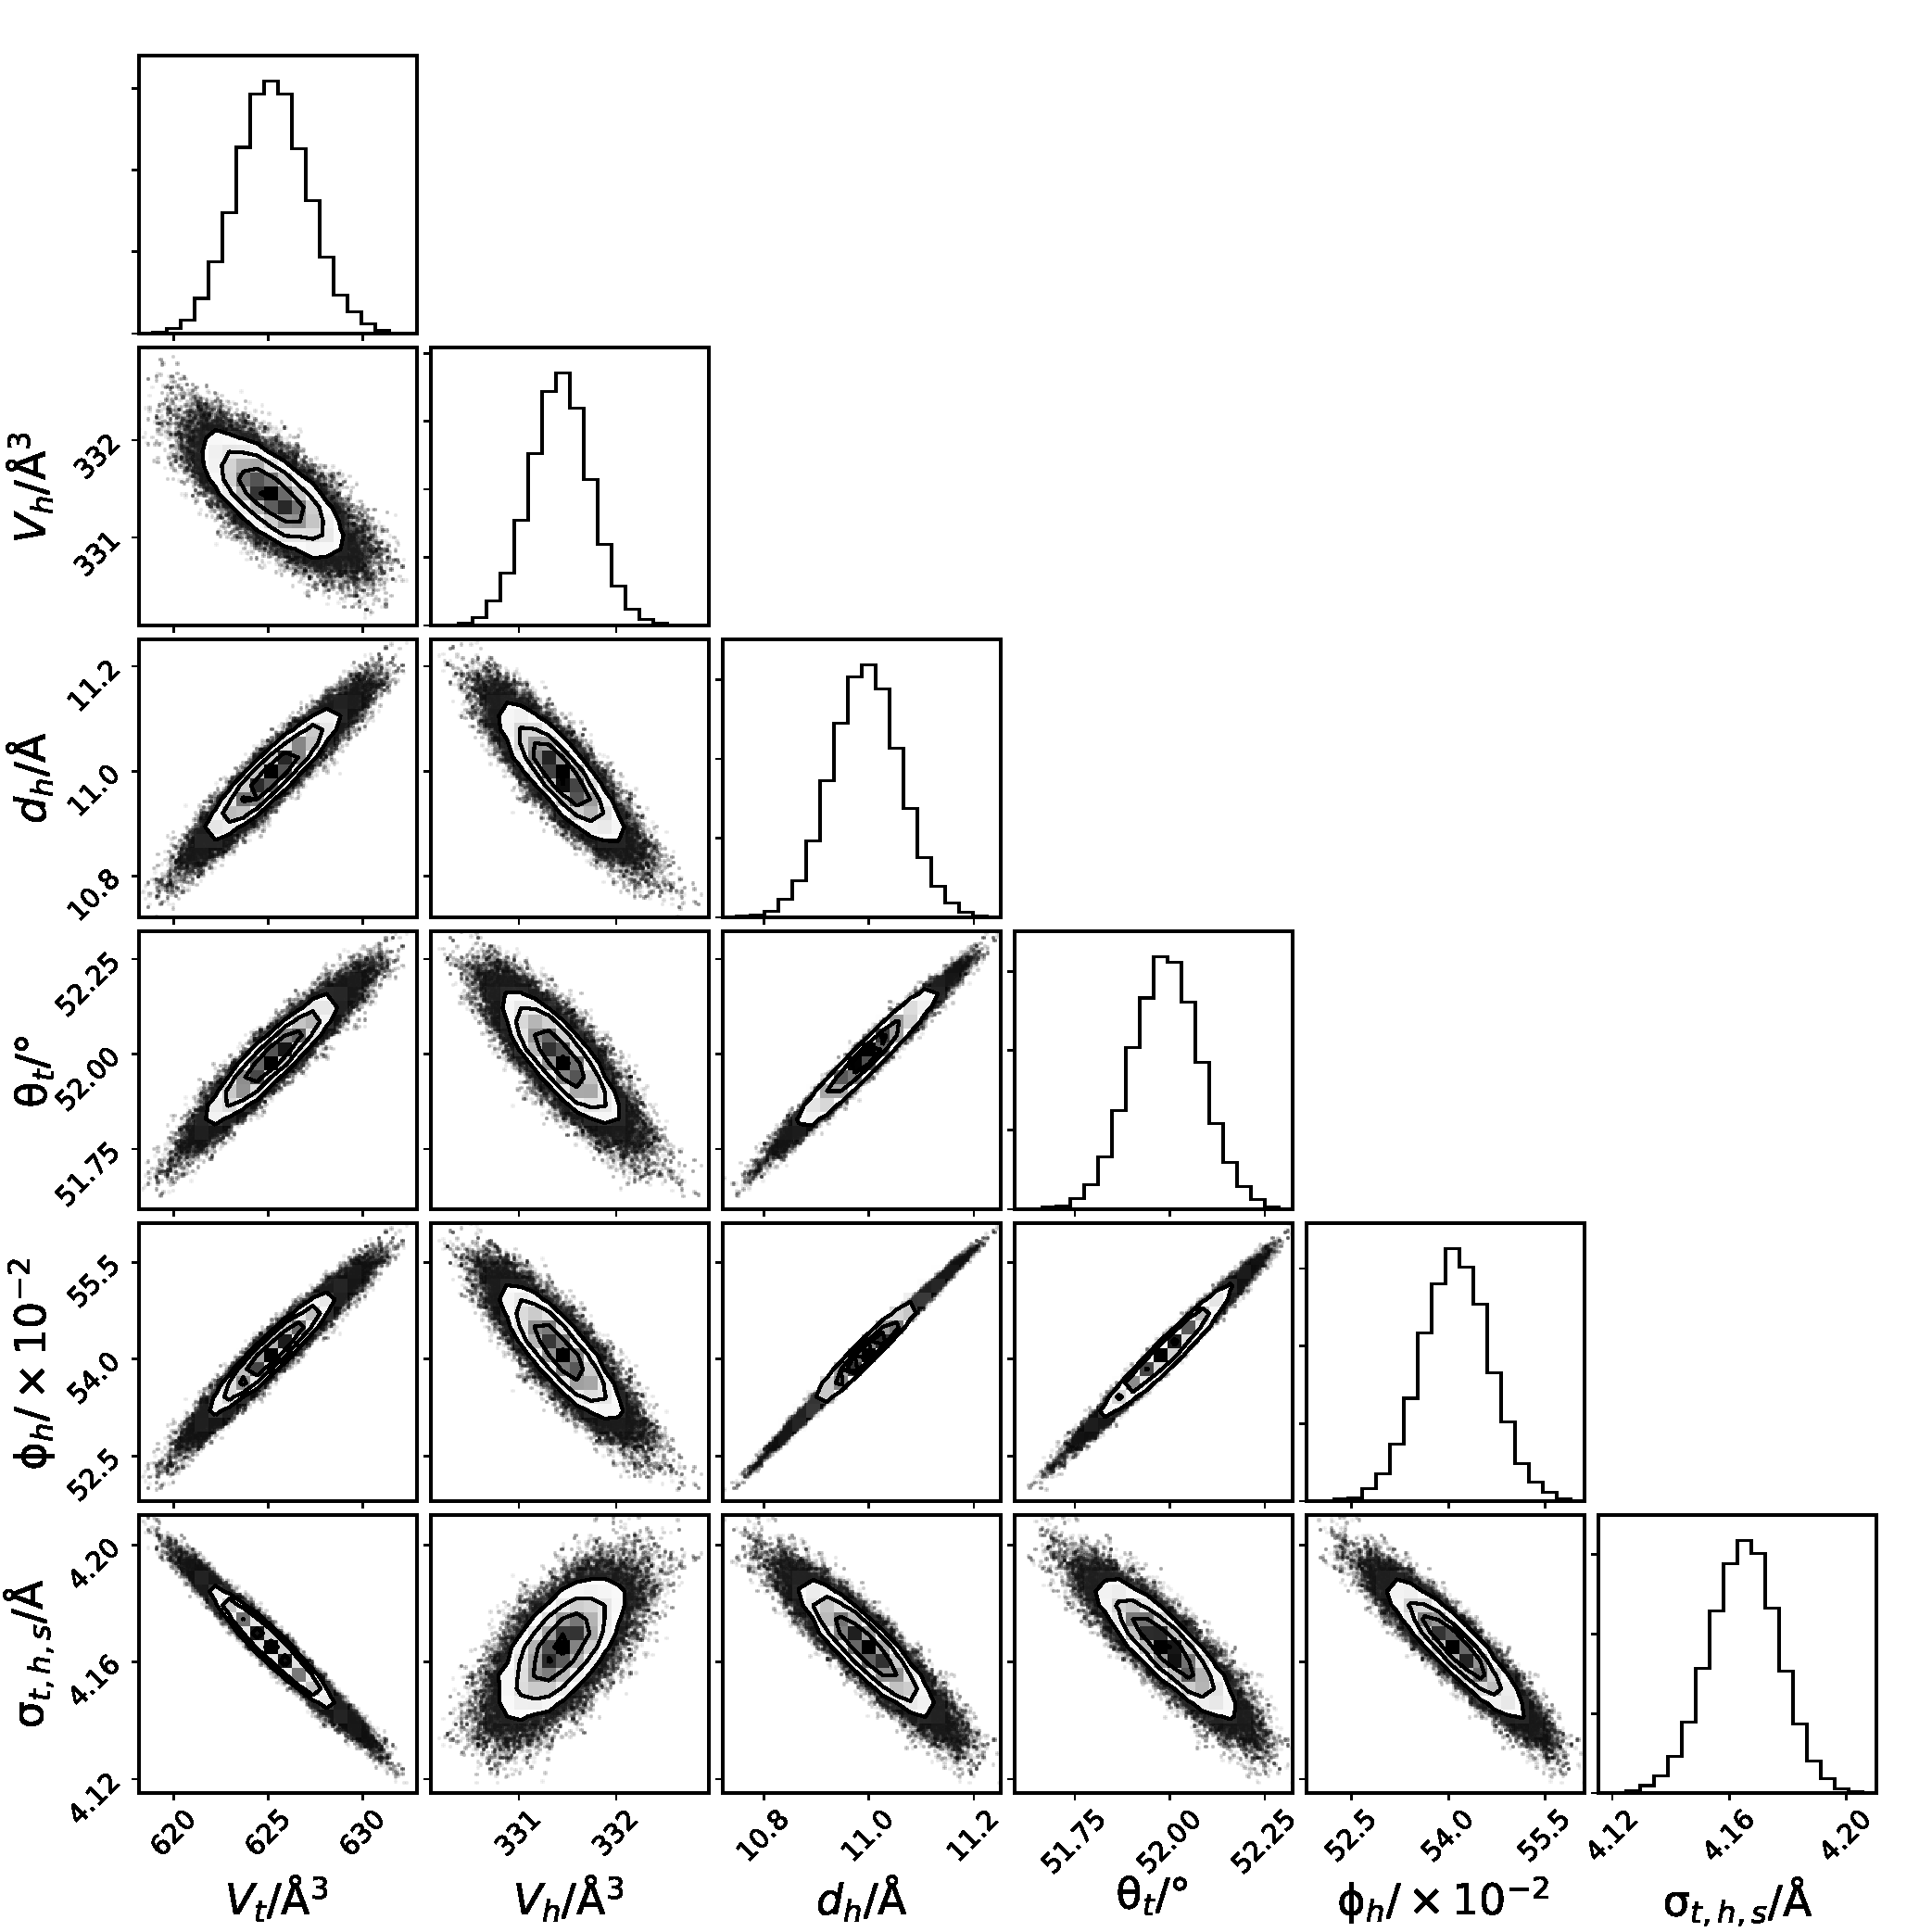
\includegraphics[width=0.50\textwidth]{figures/dlpc3_all_corner}
	\caption{The multi-parameter PDFs for the chemically-relevant model of DLPC X-ray reflectometry data at 30 mNm$^{-1}$.}
	\label{fig:dlpc4}
\end{figure}
\begin{figure}[H]
	\centering
	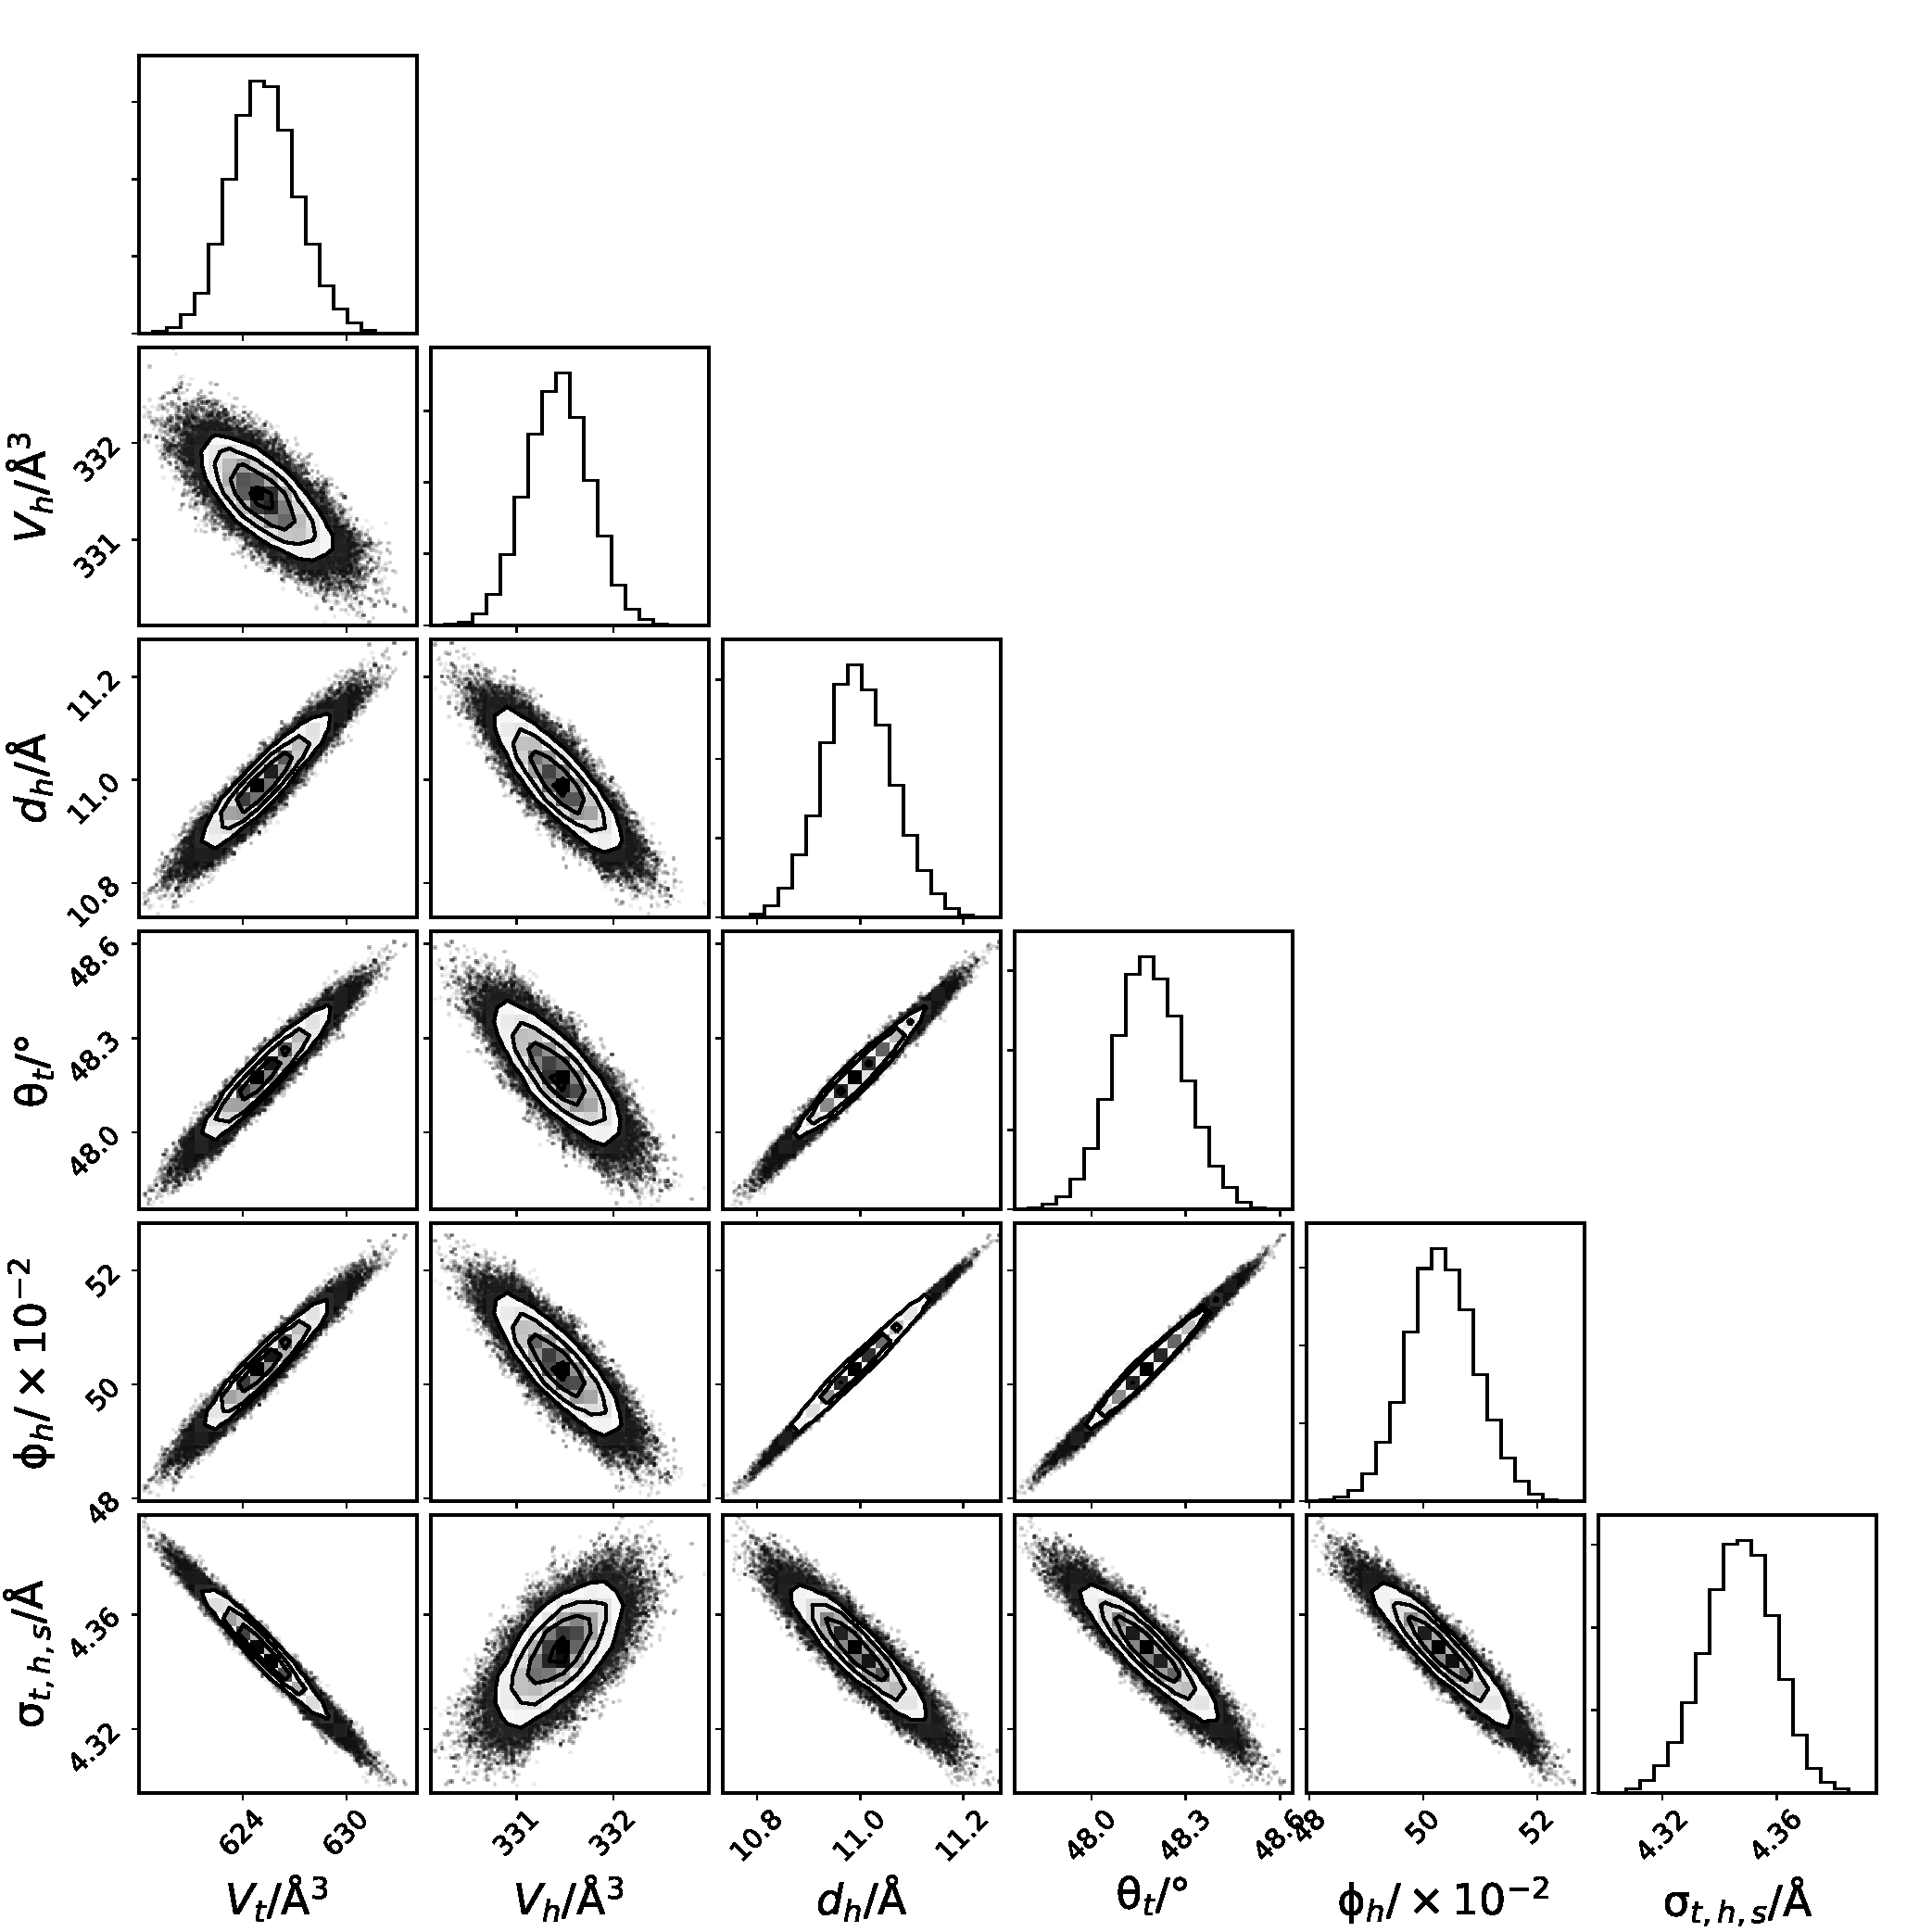
\includegraphics[width=0.50\textwidth]{figures/dlpc4_all_corner}
	\caption{The multi-parameter PDFs for the chemically-relevant model of DLPC X-ray reflectometry data at 35 mNm$^{-1}$.}
	\label{fig:dlpc5}
\end{figure}
\begin{figure}[H]
	\centering
	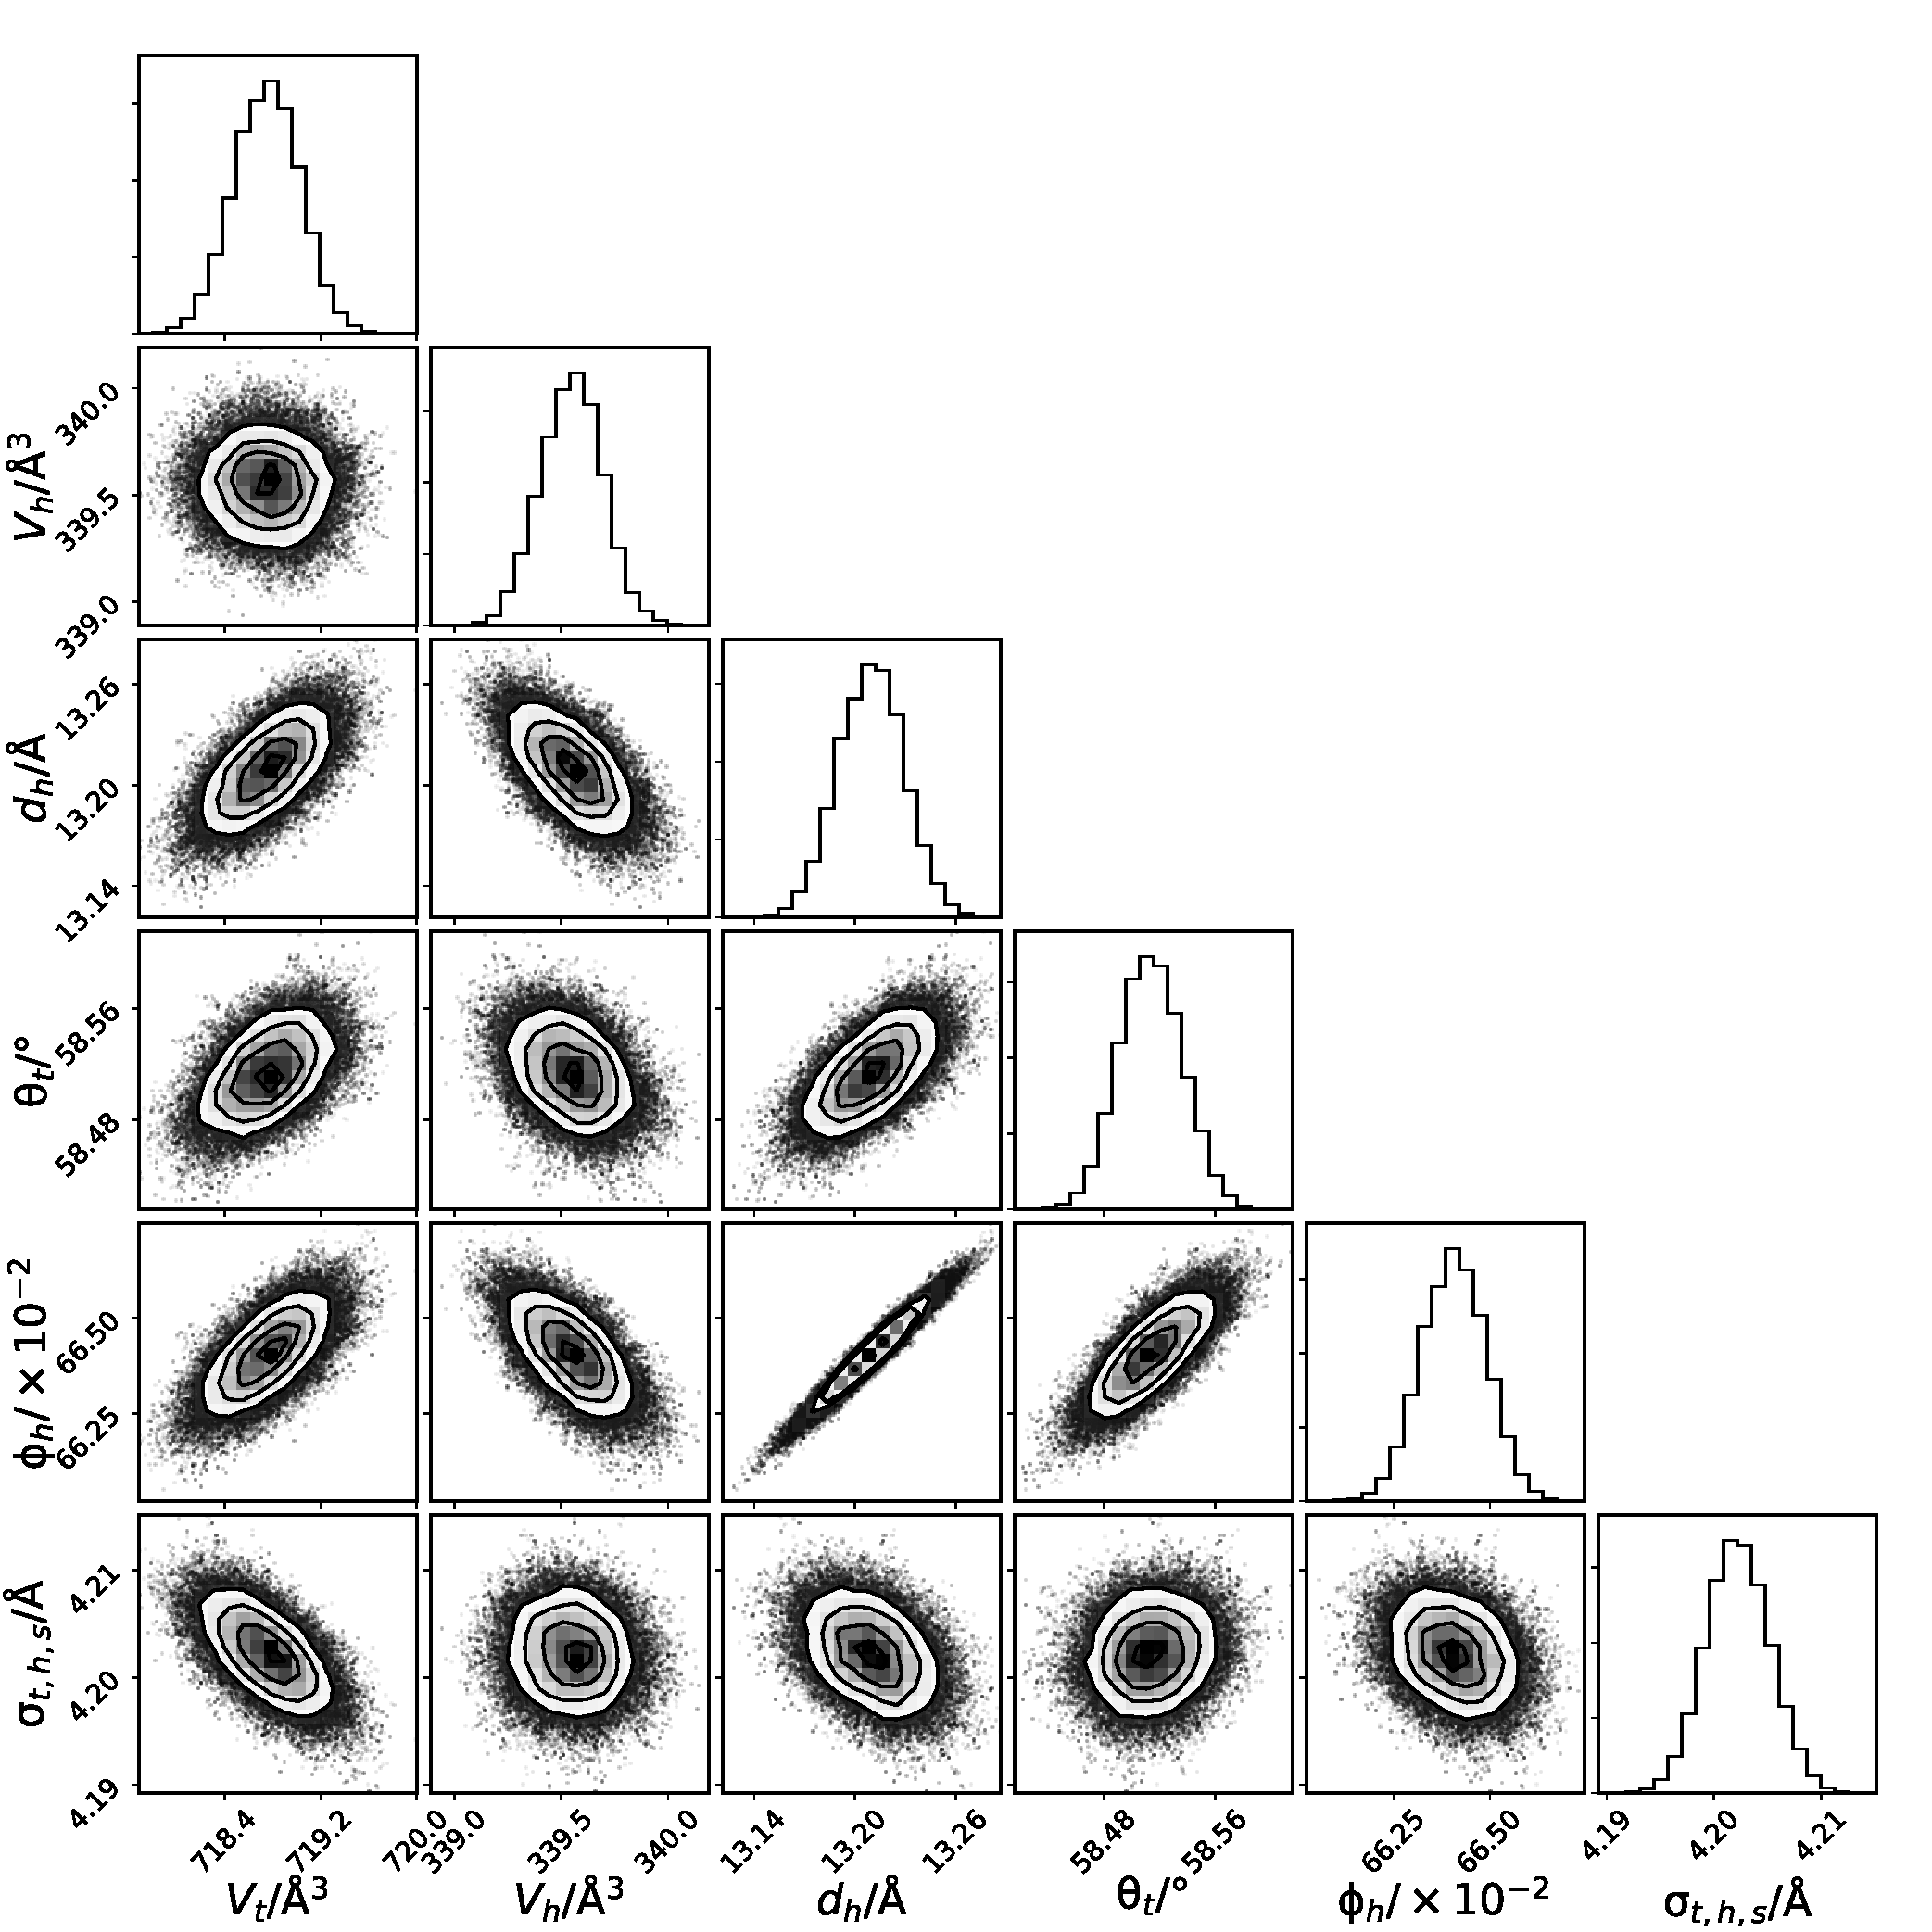
\includegraphics[width=0.50\textwidth]{figures/dmpc1_all_corner}
	\caption{The multi-parameter PDFs for the chemically-relevant model of DMPC X-ray reflectometry data at 20 mNm$^{-1}$.}
	\label{fig:dmpc2}
\end{figure}
\begin{figure}[H]
	\centering
	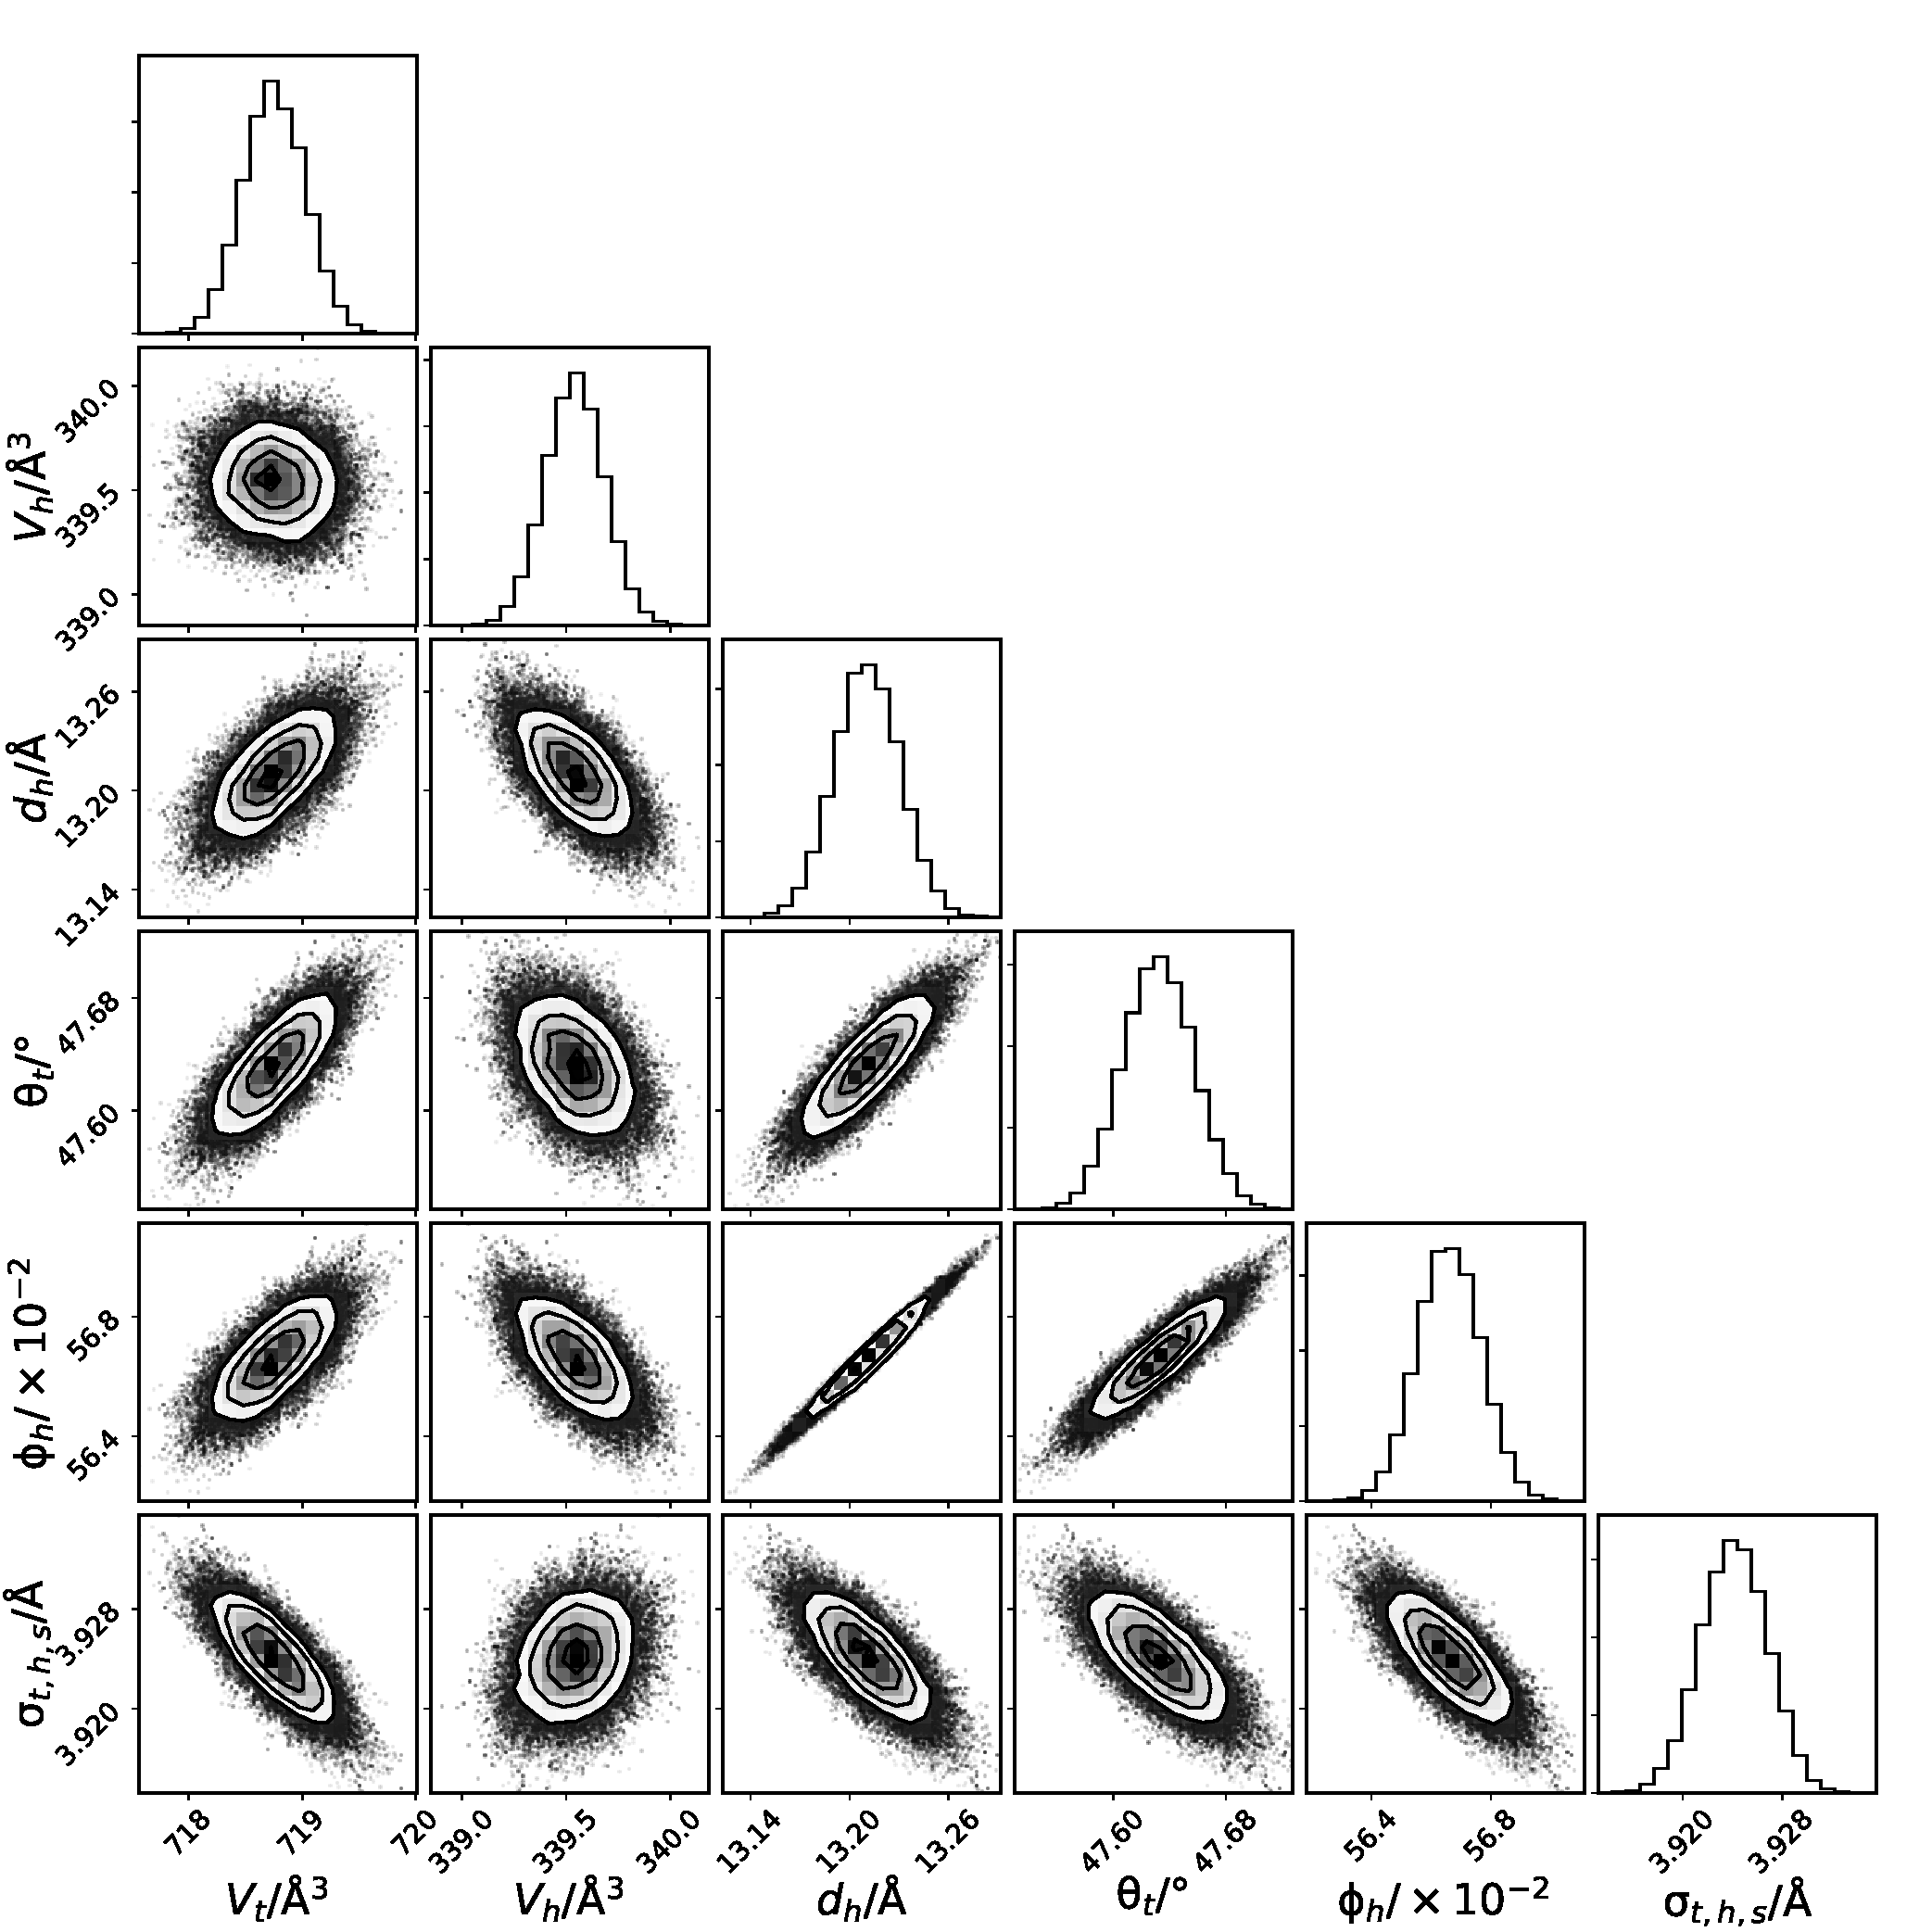
\includegraphics[width=0.50\textwidth]{figures/dmpc2_all_corner}
	\caption{The multi-parameter PDFs for the chemically-relevant model of DMPC X-ray reflectometry data at 25 mNm$^{-1}$.}
	\label{fig:dmpc3}
\end{figure}
\begin{figure}[H]
	\centering
	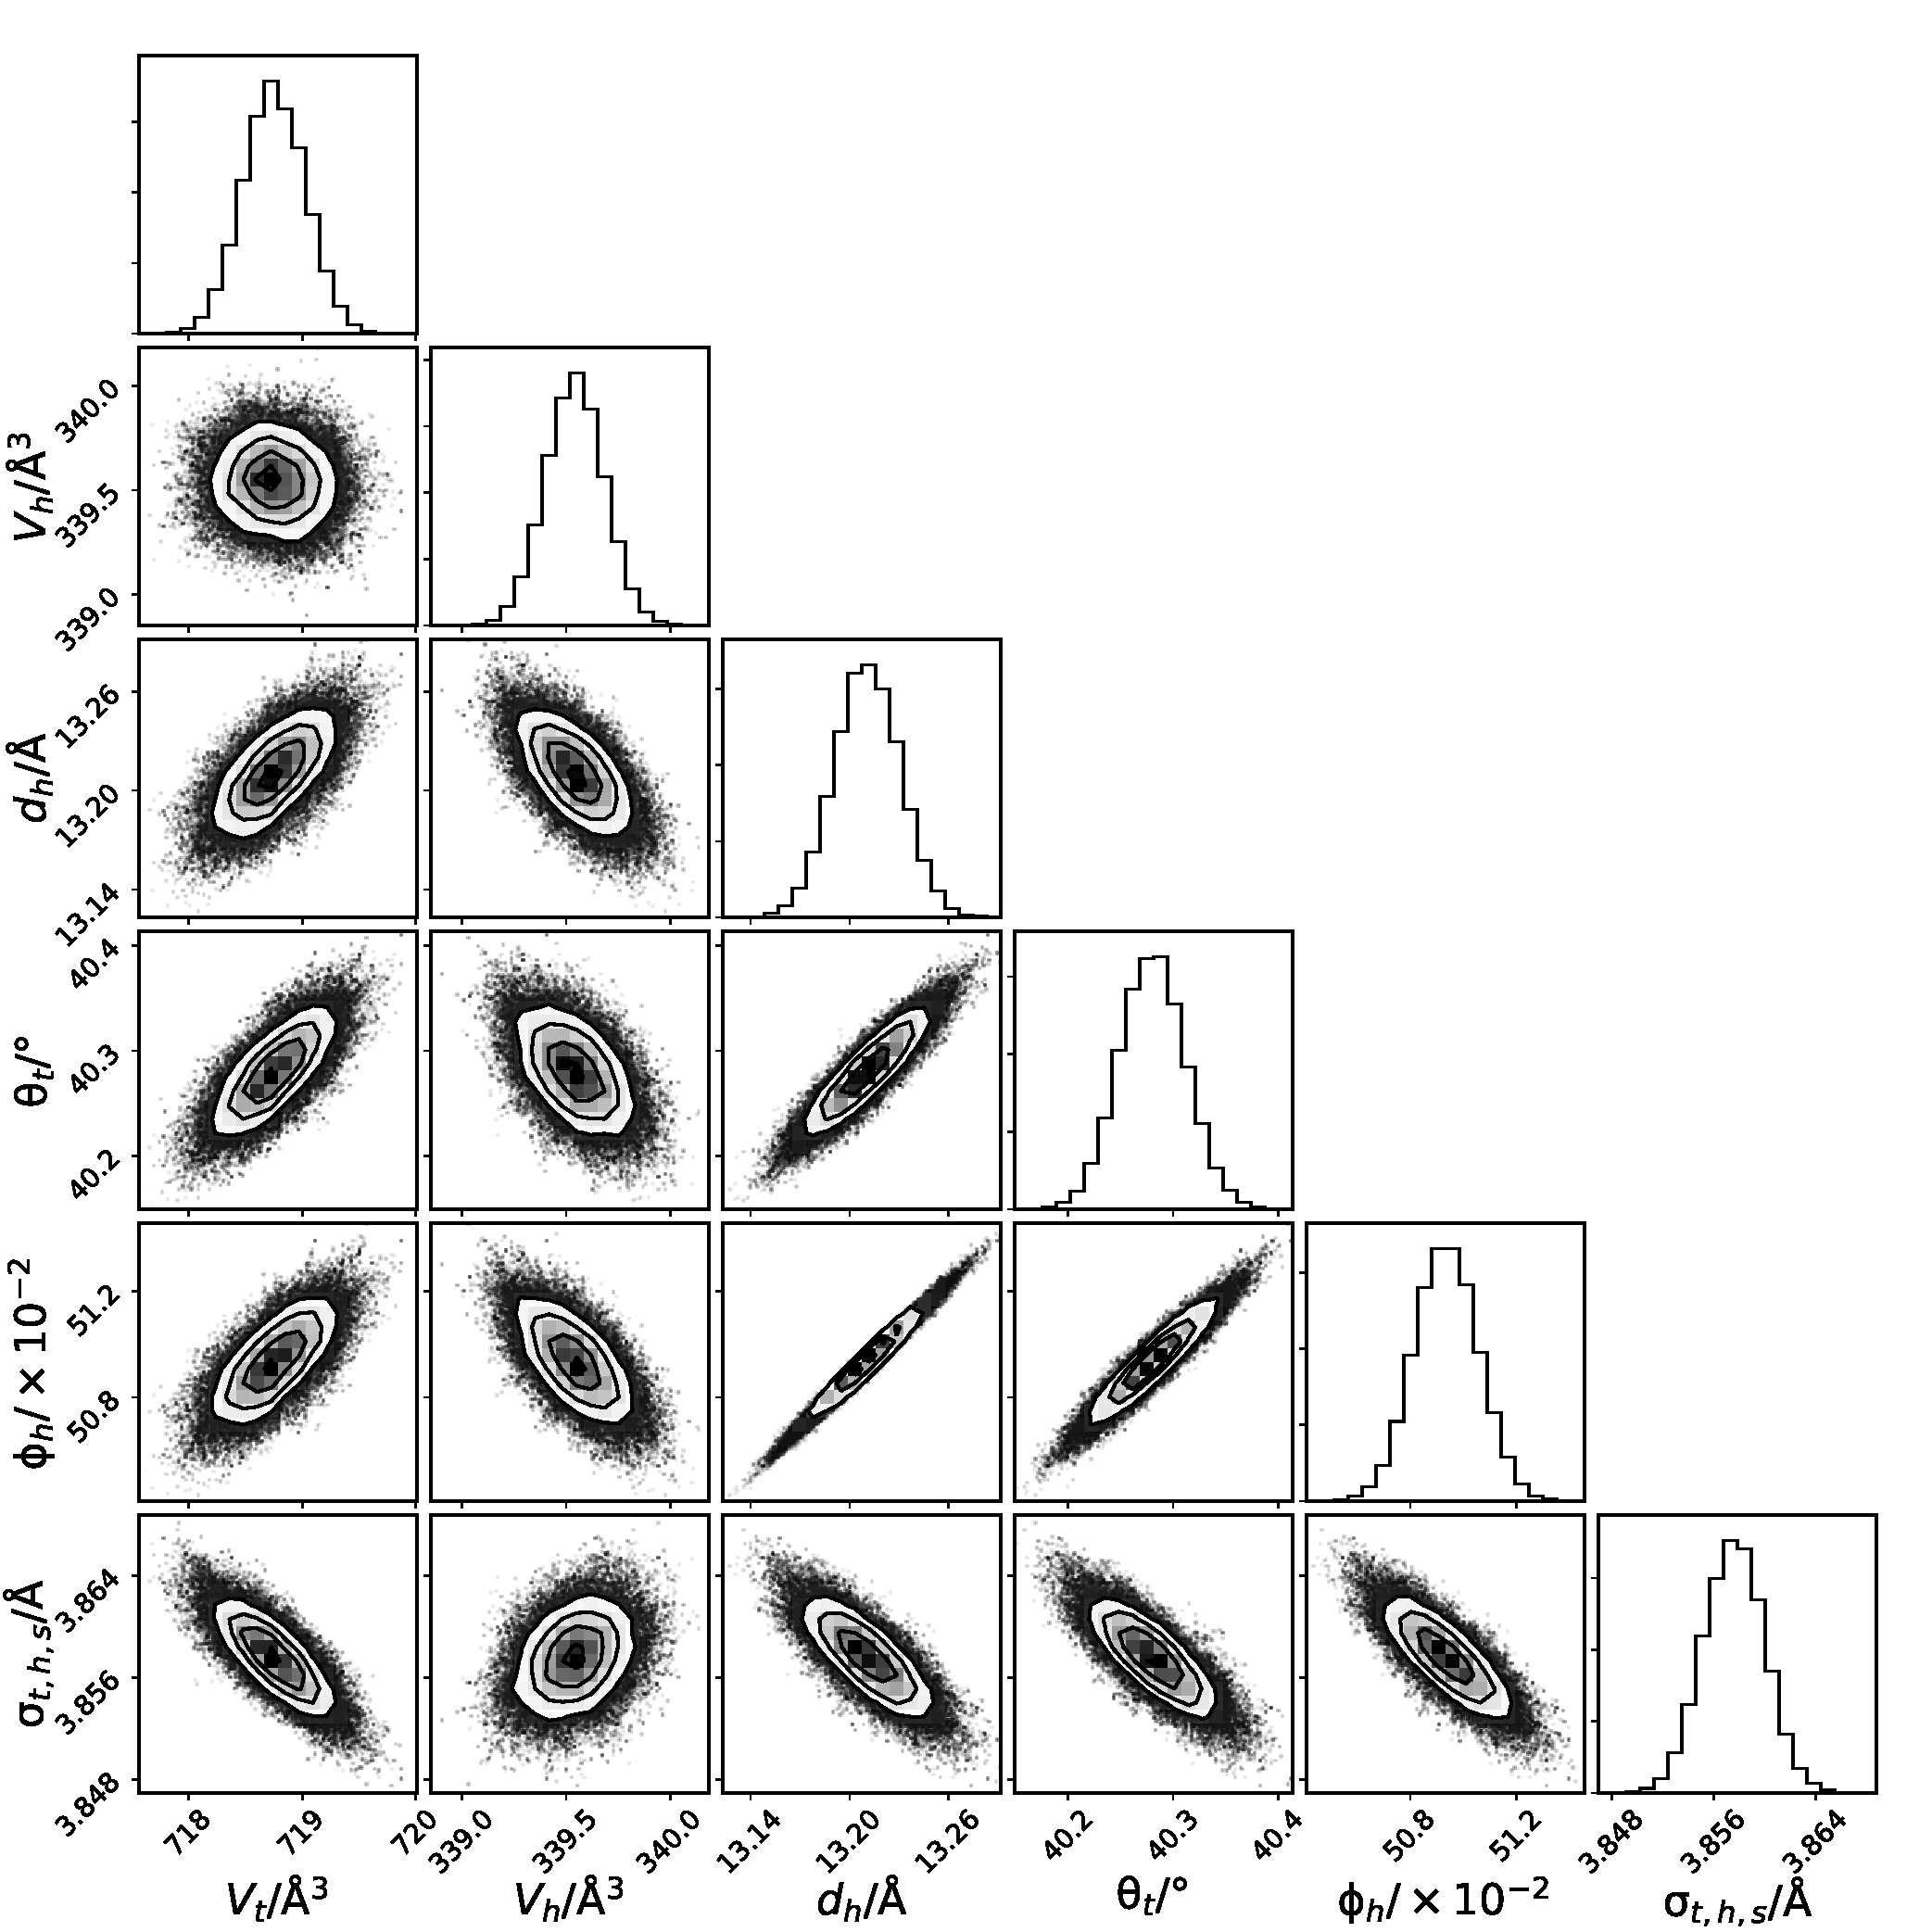
\includegraphics[width=0.50\textwidth]{figures/dmpc3_all_corner}
	\caption{The multi-parameter PDFs for the chemically-relevant model of DMPC X-ray reflectometry data at 30 mNm$^{-1}$.}
	\label{fig:dmpc4}
\end{figure}
\begin{figure}[H]
	\centering
	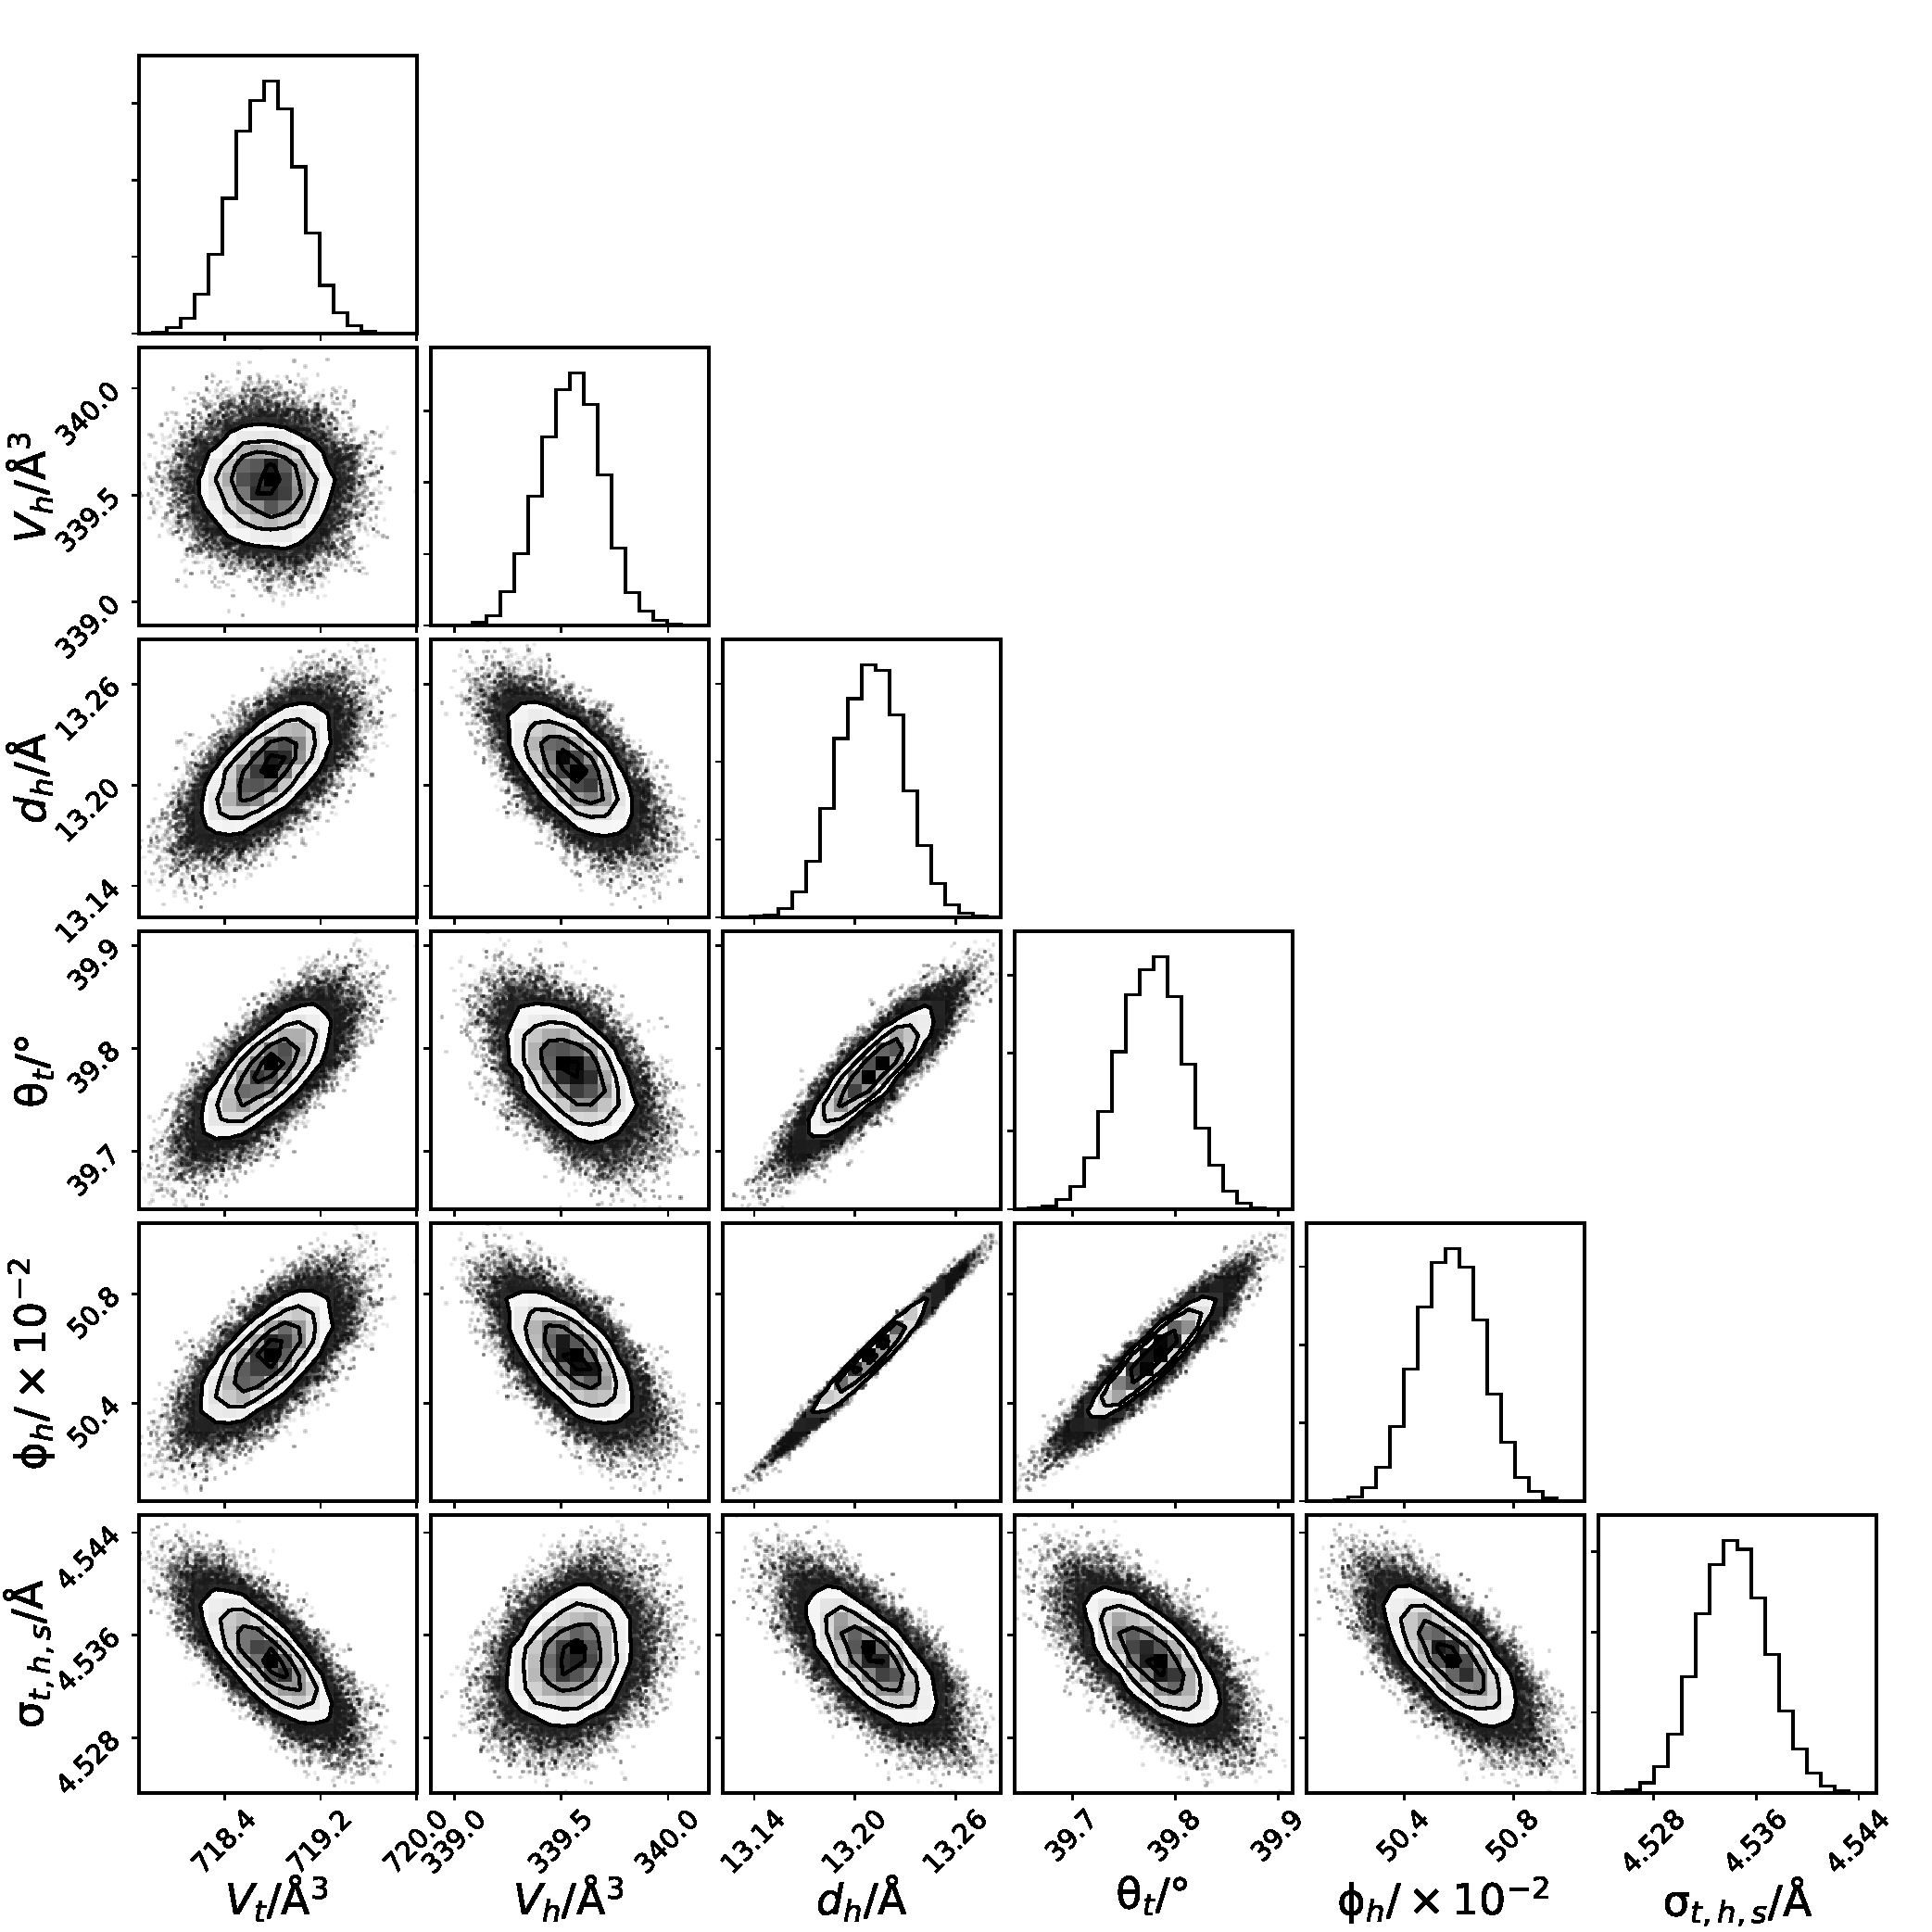
\includegraphics[width=0.50\textwidth]{figures/dmpc4_all_corner}
	\caption{The multi-parameter PDFs for the chemically-relevant model of DMPC X-ray reflectometry data at 40 mNm$^{-1}$.}
	\label{fig:dmpc5}
\end{figure}
\begin{figure}[H]
	\centering
	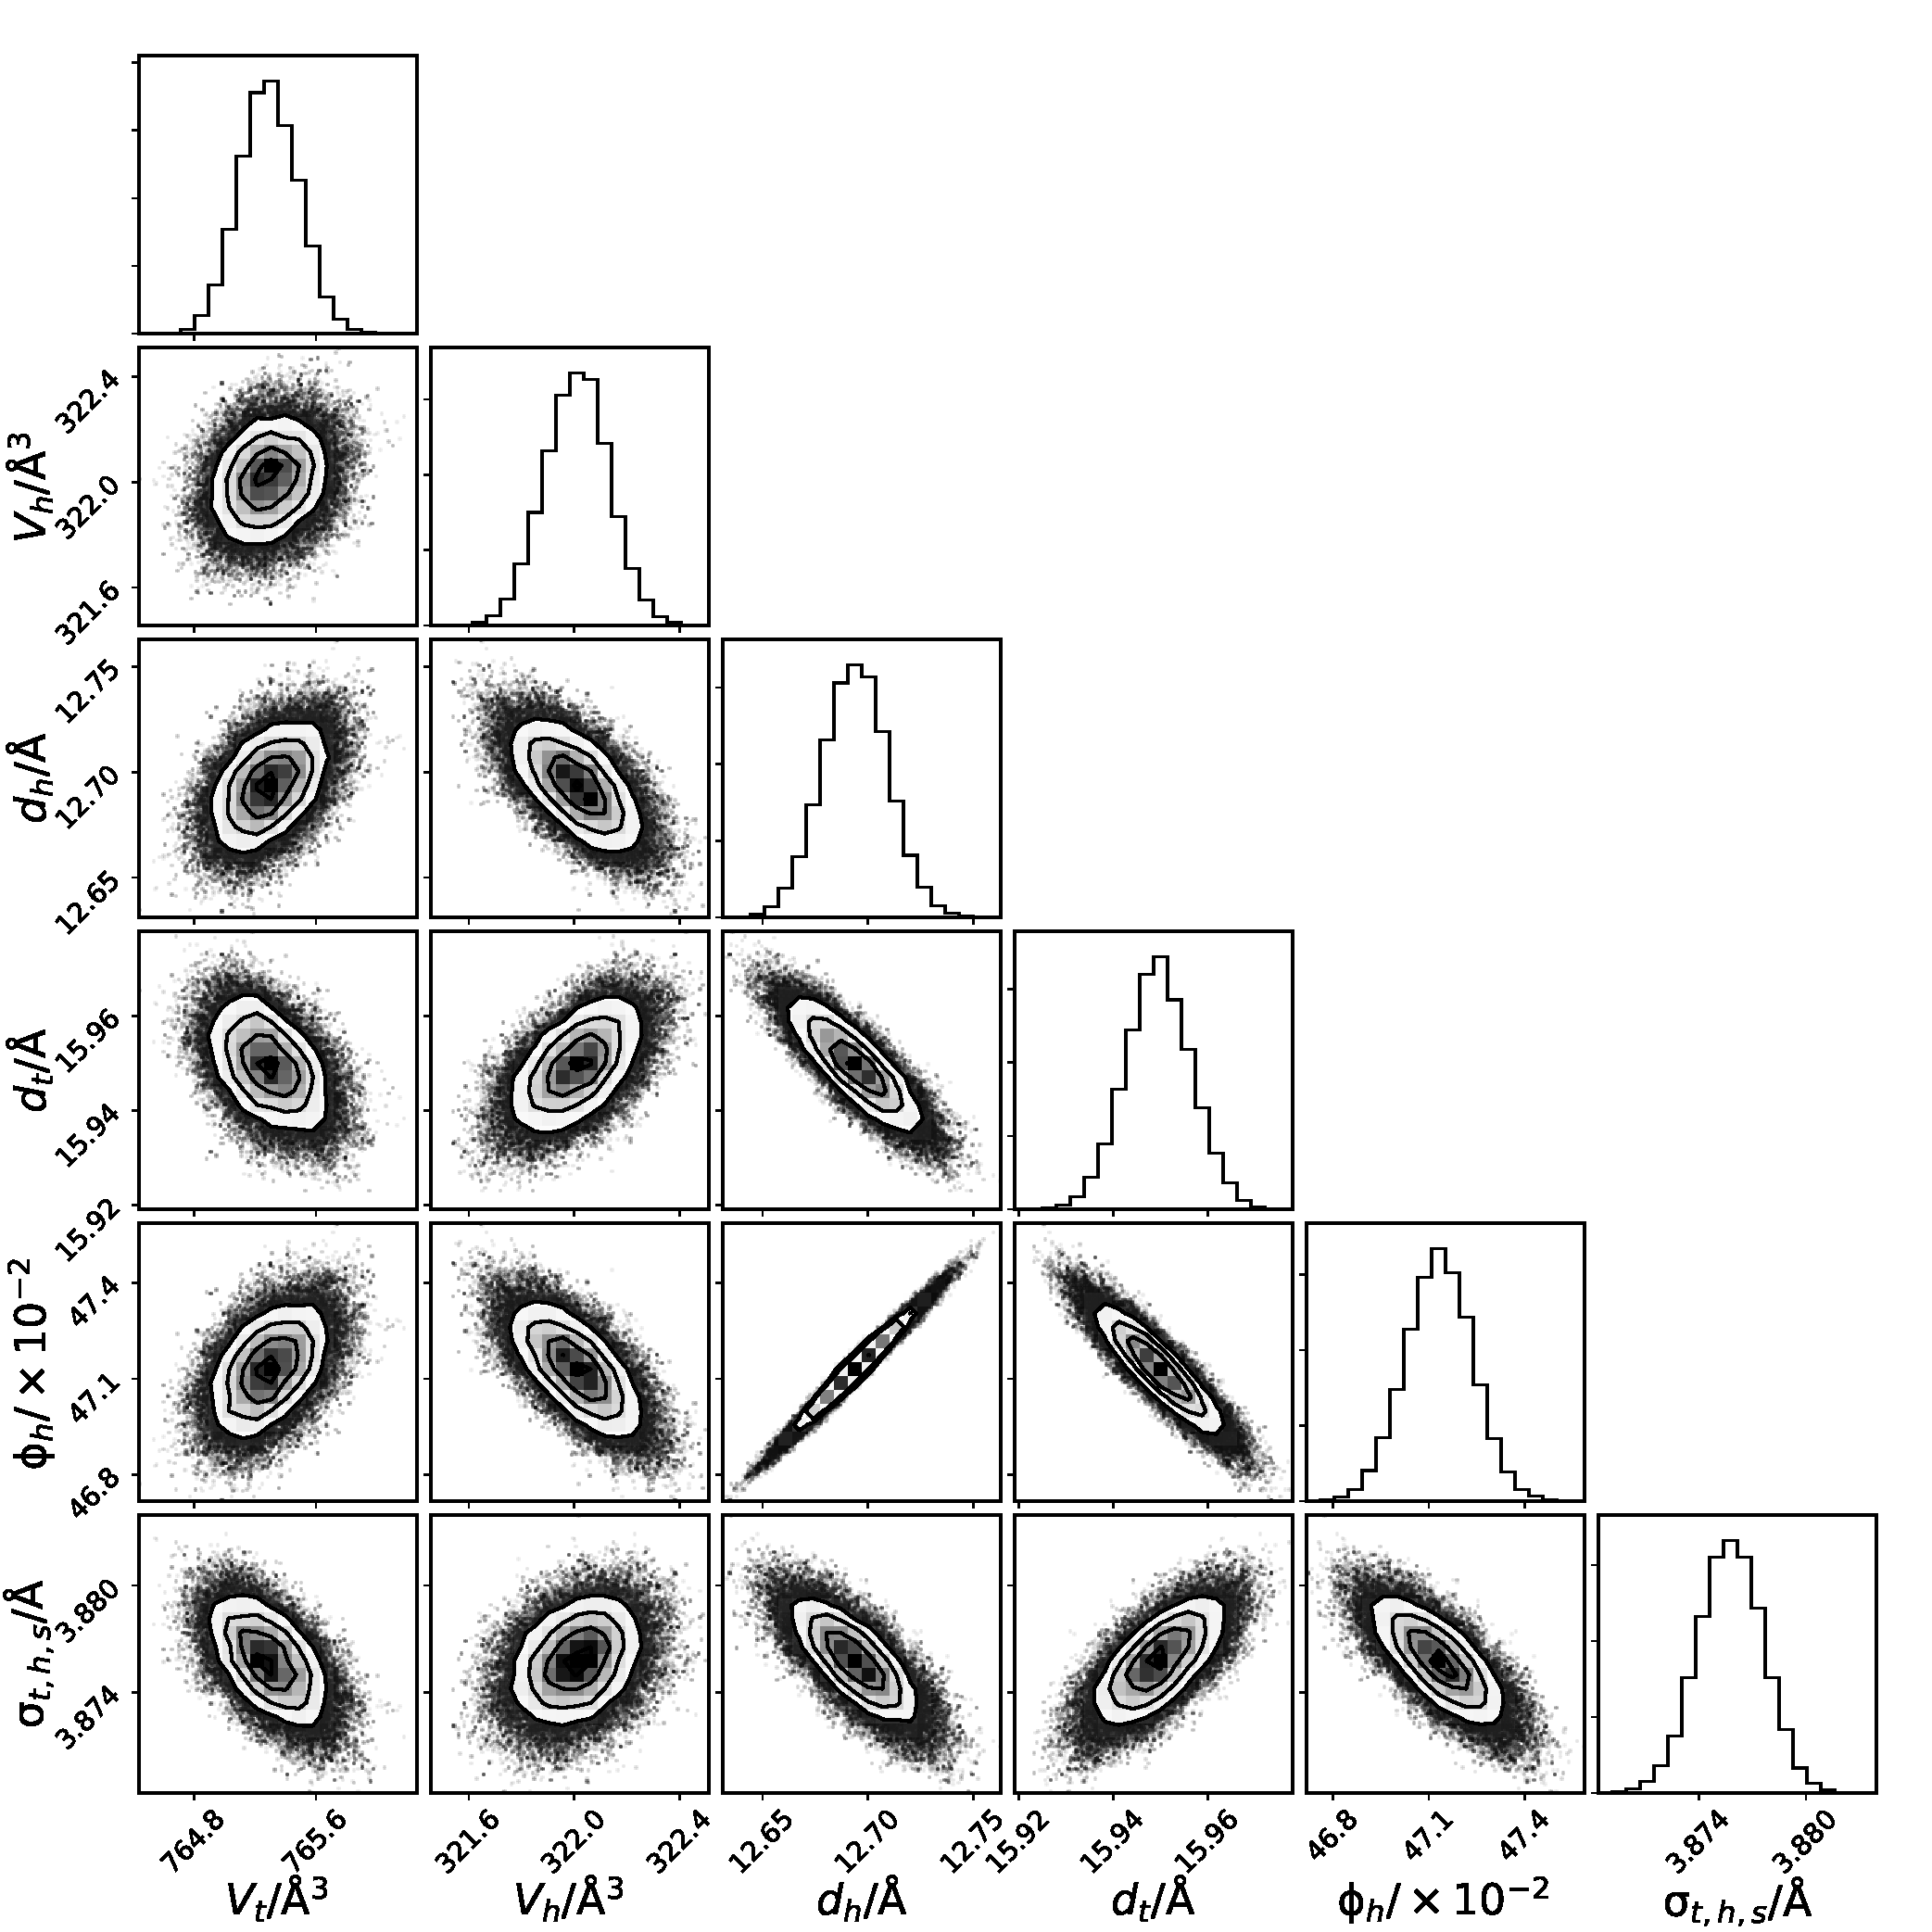
\includegraphics[width=0.50\textwidth]{figures/dppc1_all_corner}
	\caption{The multi-parameter PDFs for the chemically-relevant model of DPPC X-ray reflectometry data at 15 mNm$^{-1}$.}
	\label{fig:dppc2}
\end{figure}
\begin{figure}[H]
	\centering
	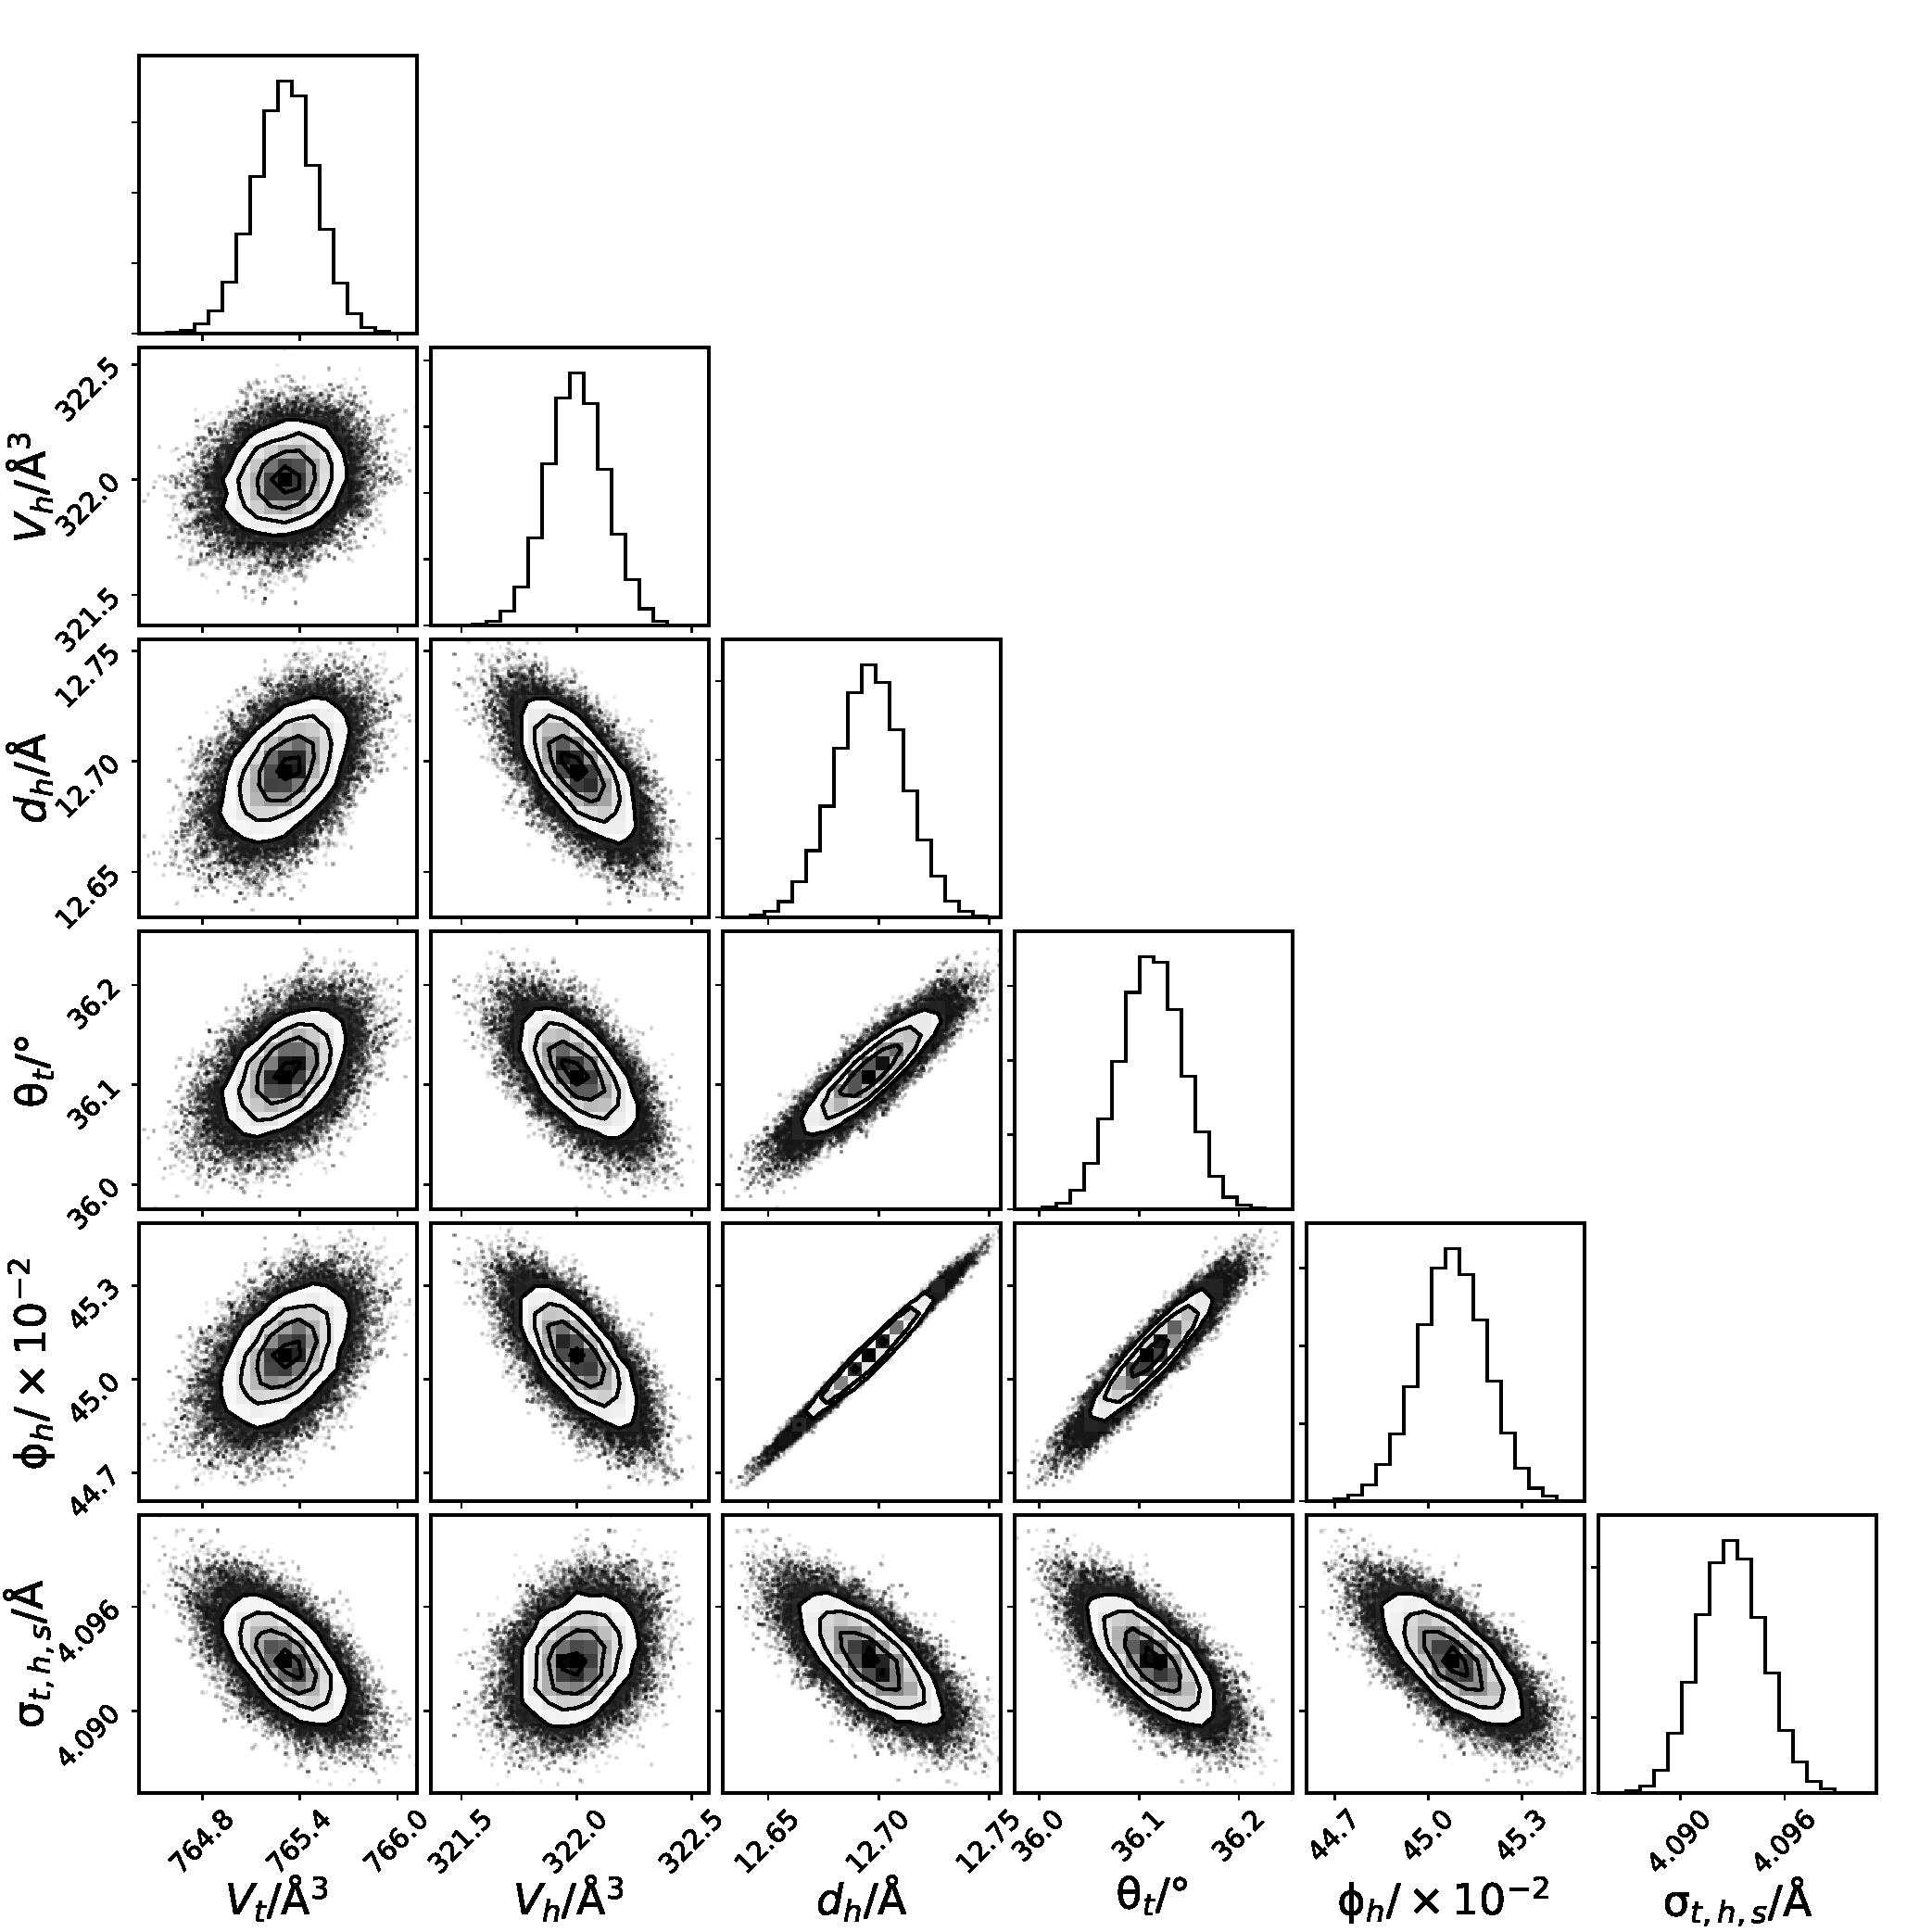
\includegraphics[width=0.50\textwidth]{figures/dppc2_all_corner}
	\caption{The multi-parameter PDFs for the chemically-relevant model of DPPC X-ray reflectometry data at 20 mNm$^{-1}$.}
	\label{fig:dppc3}
\end{figure}
\begin{figure}[H]
	\centering
	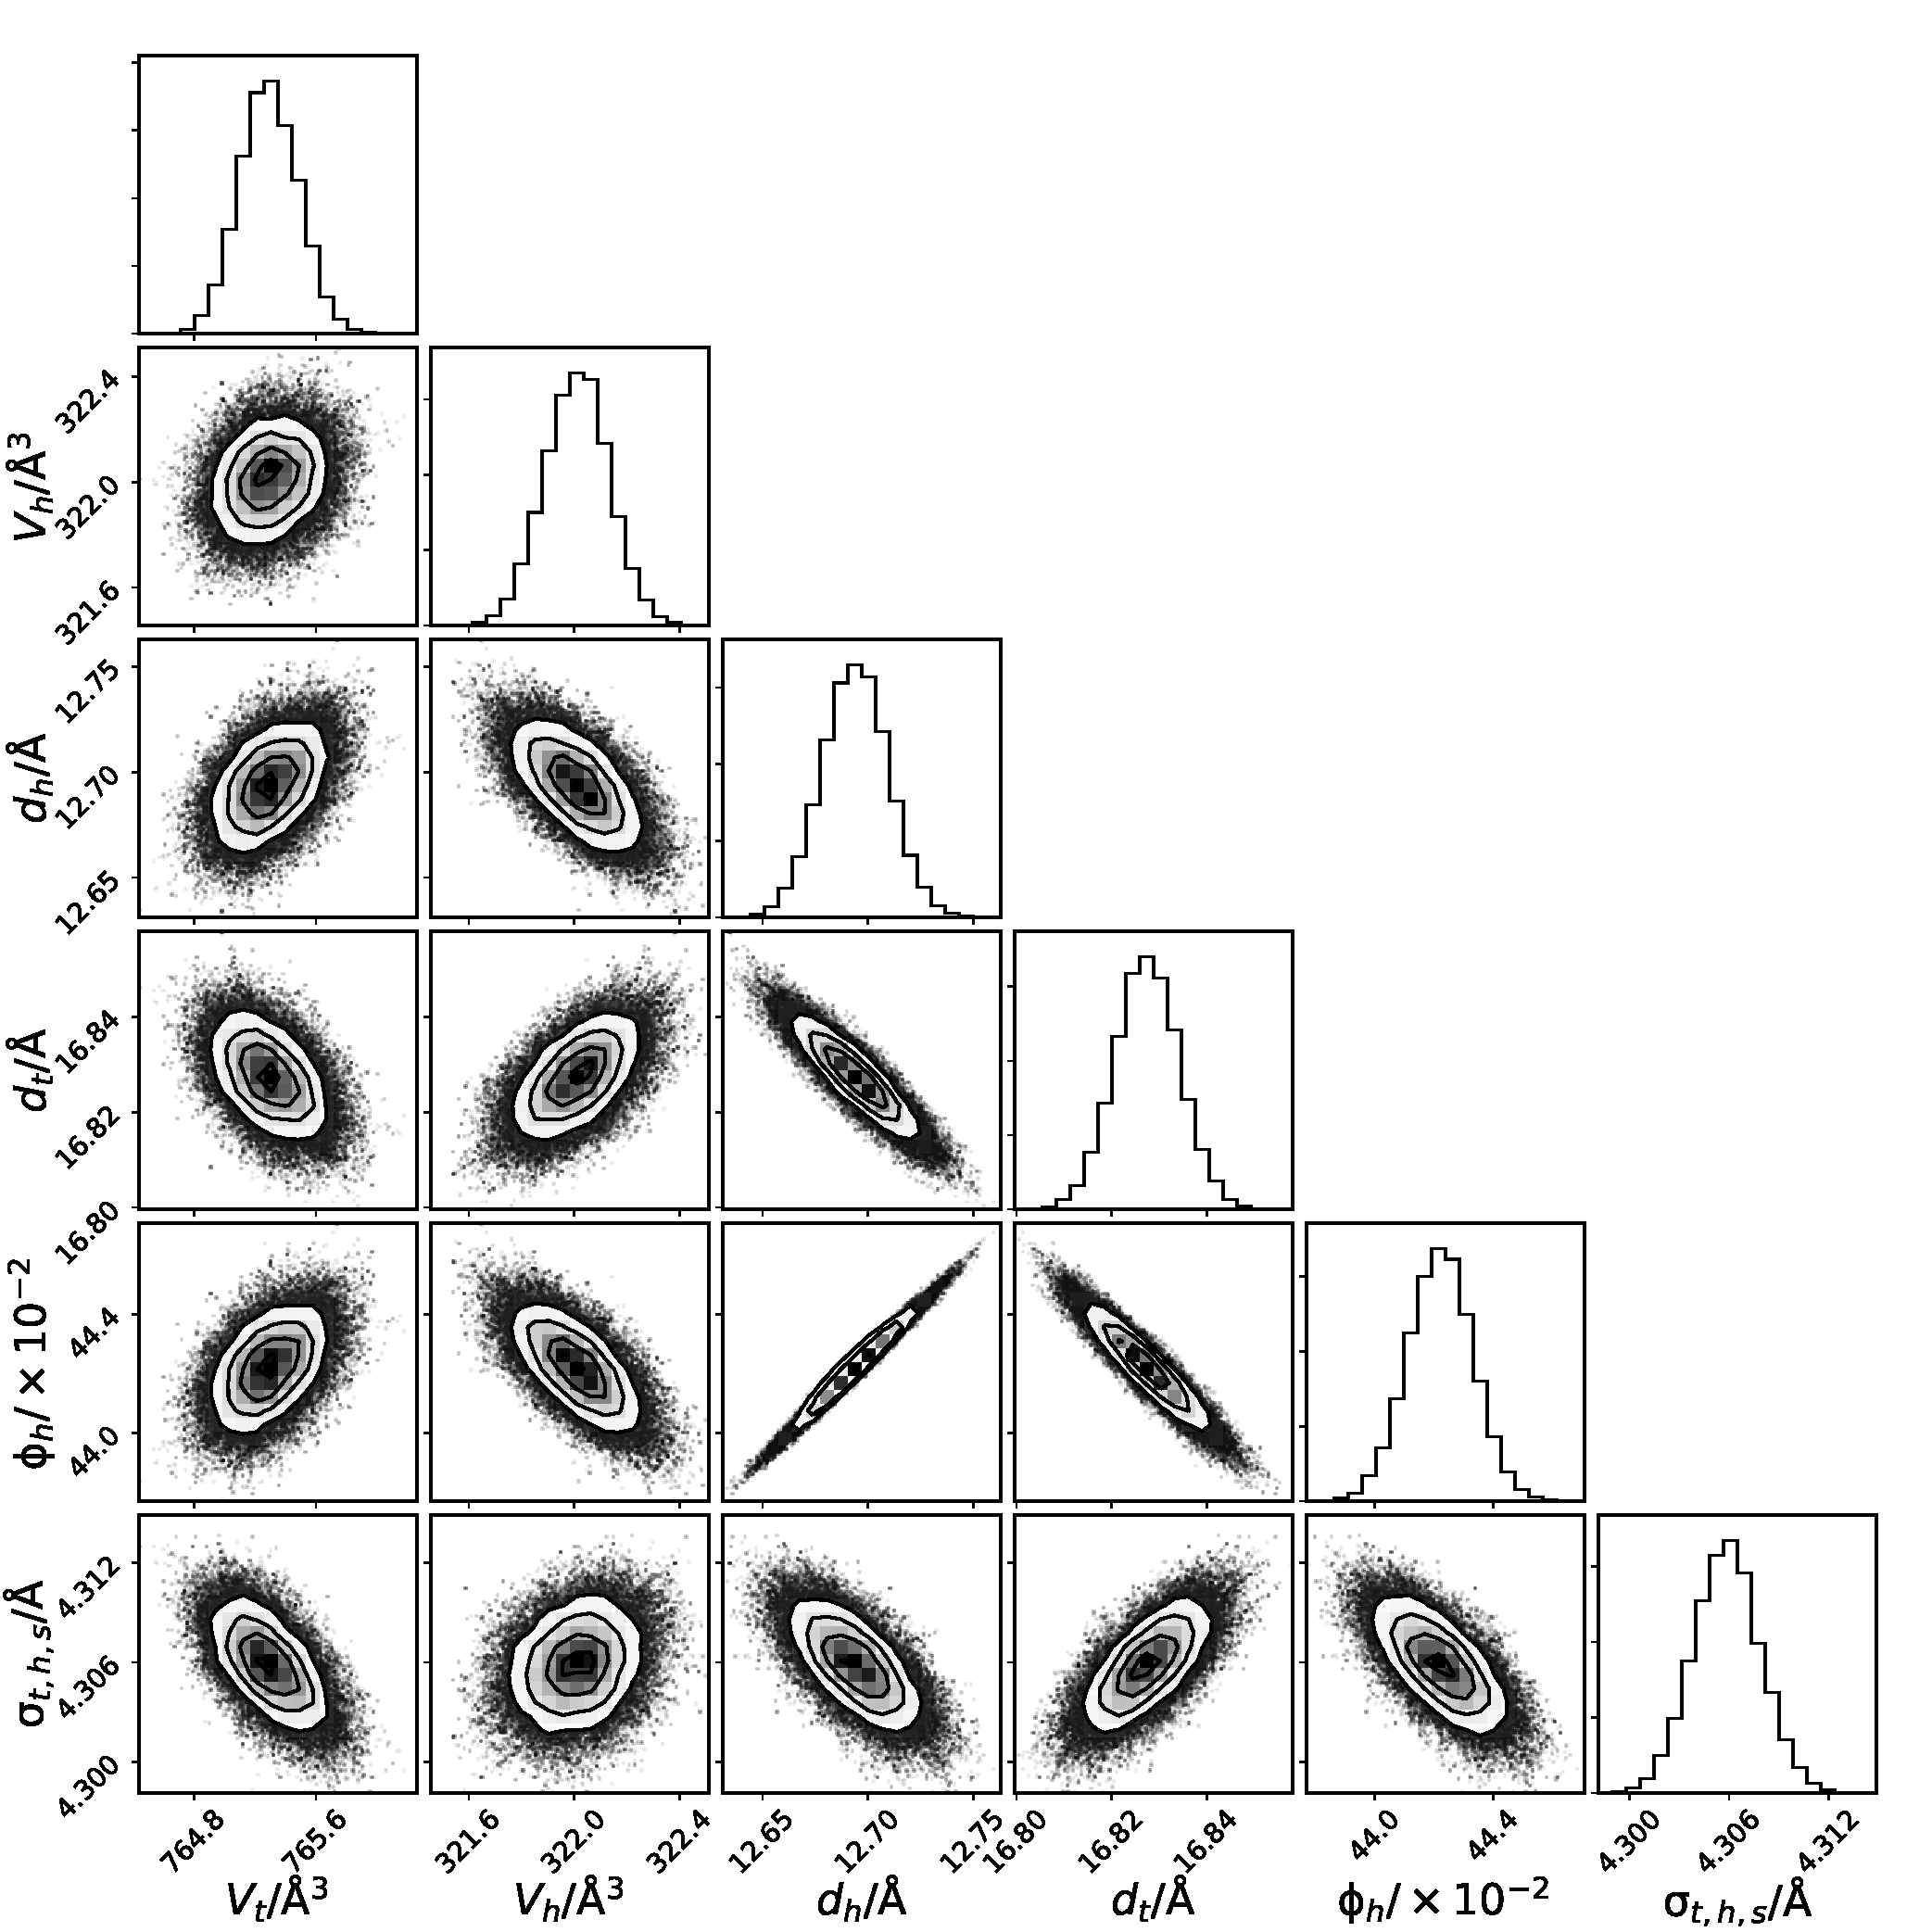
\includegraphics[width=0.50\textwidth]{figures/dppc3_all_corner}
	\caption{The multi-parameter PDFs for the chemically-relevant model of DPPC X-ray reflectometry data at 25 mNm$^{-1}$.}
	\label{fig:dppc4}
\end{figure}
\begin{figure}[H]
	\centering
	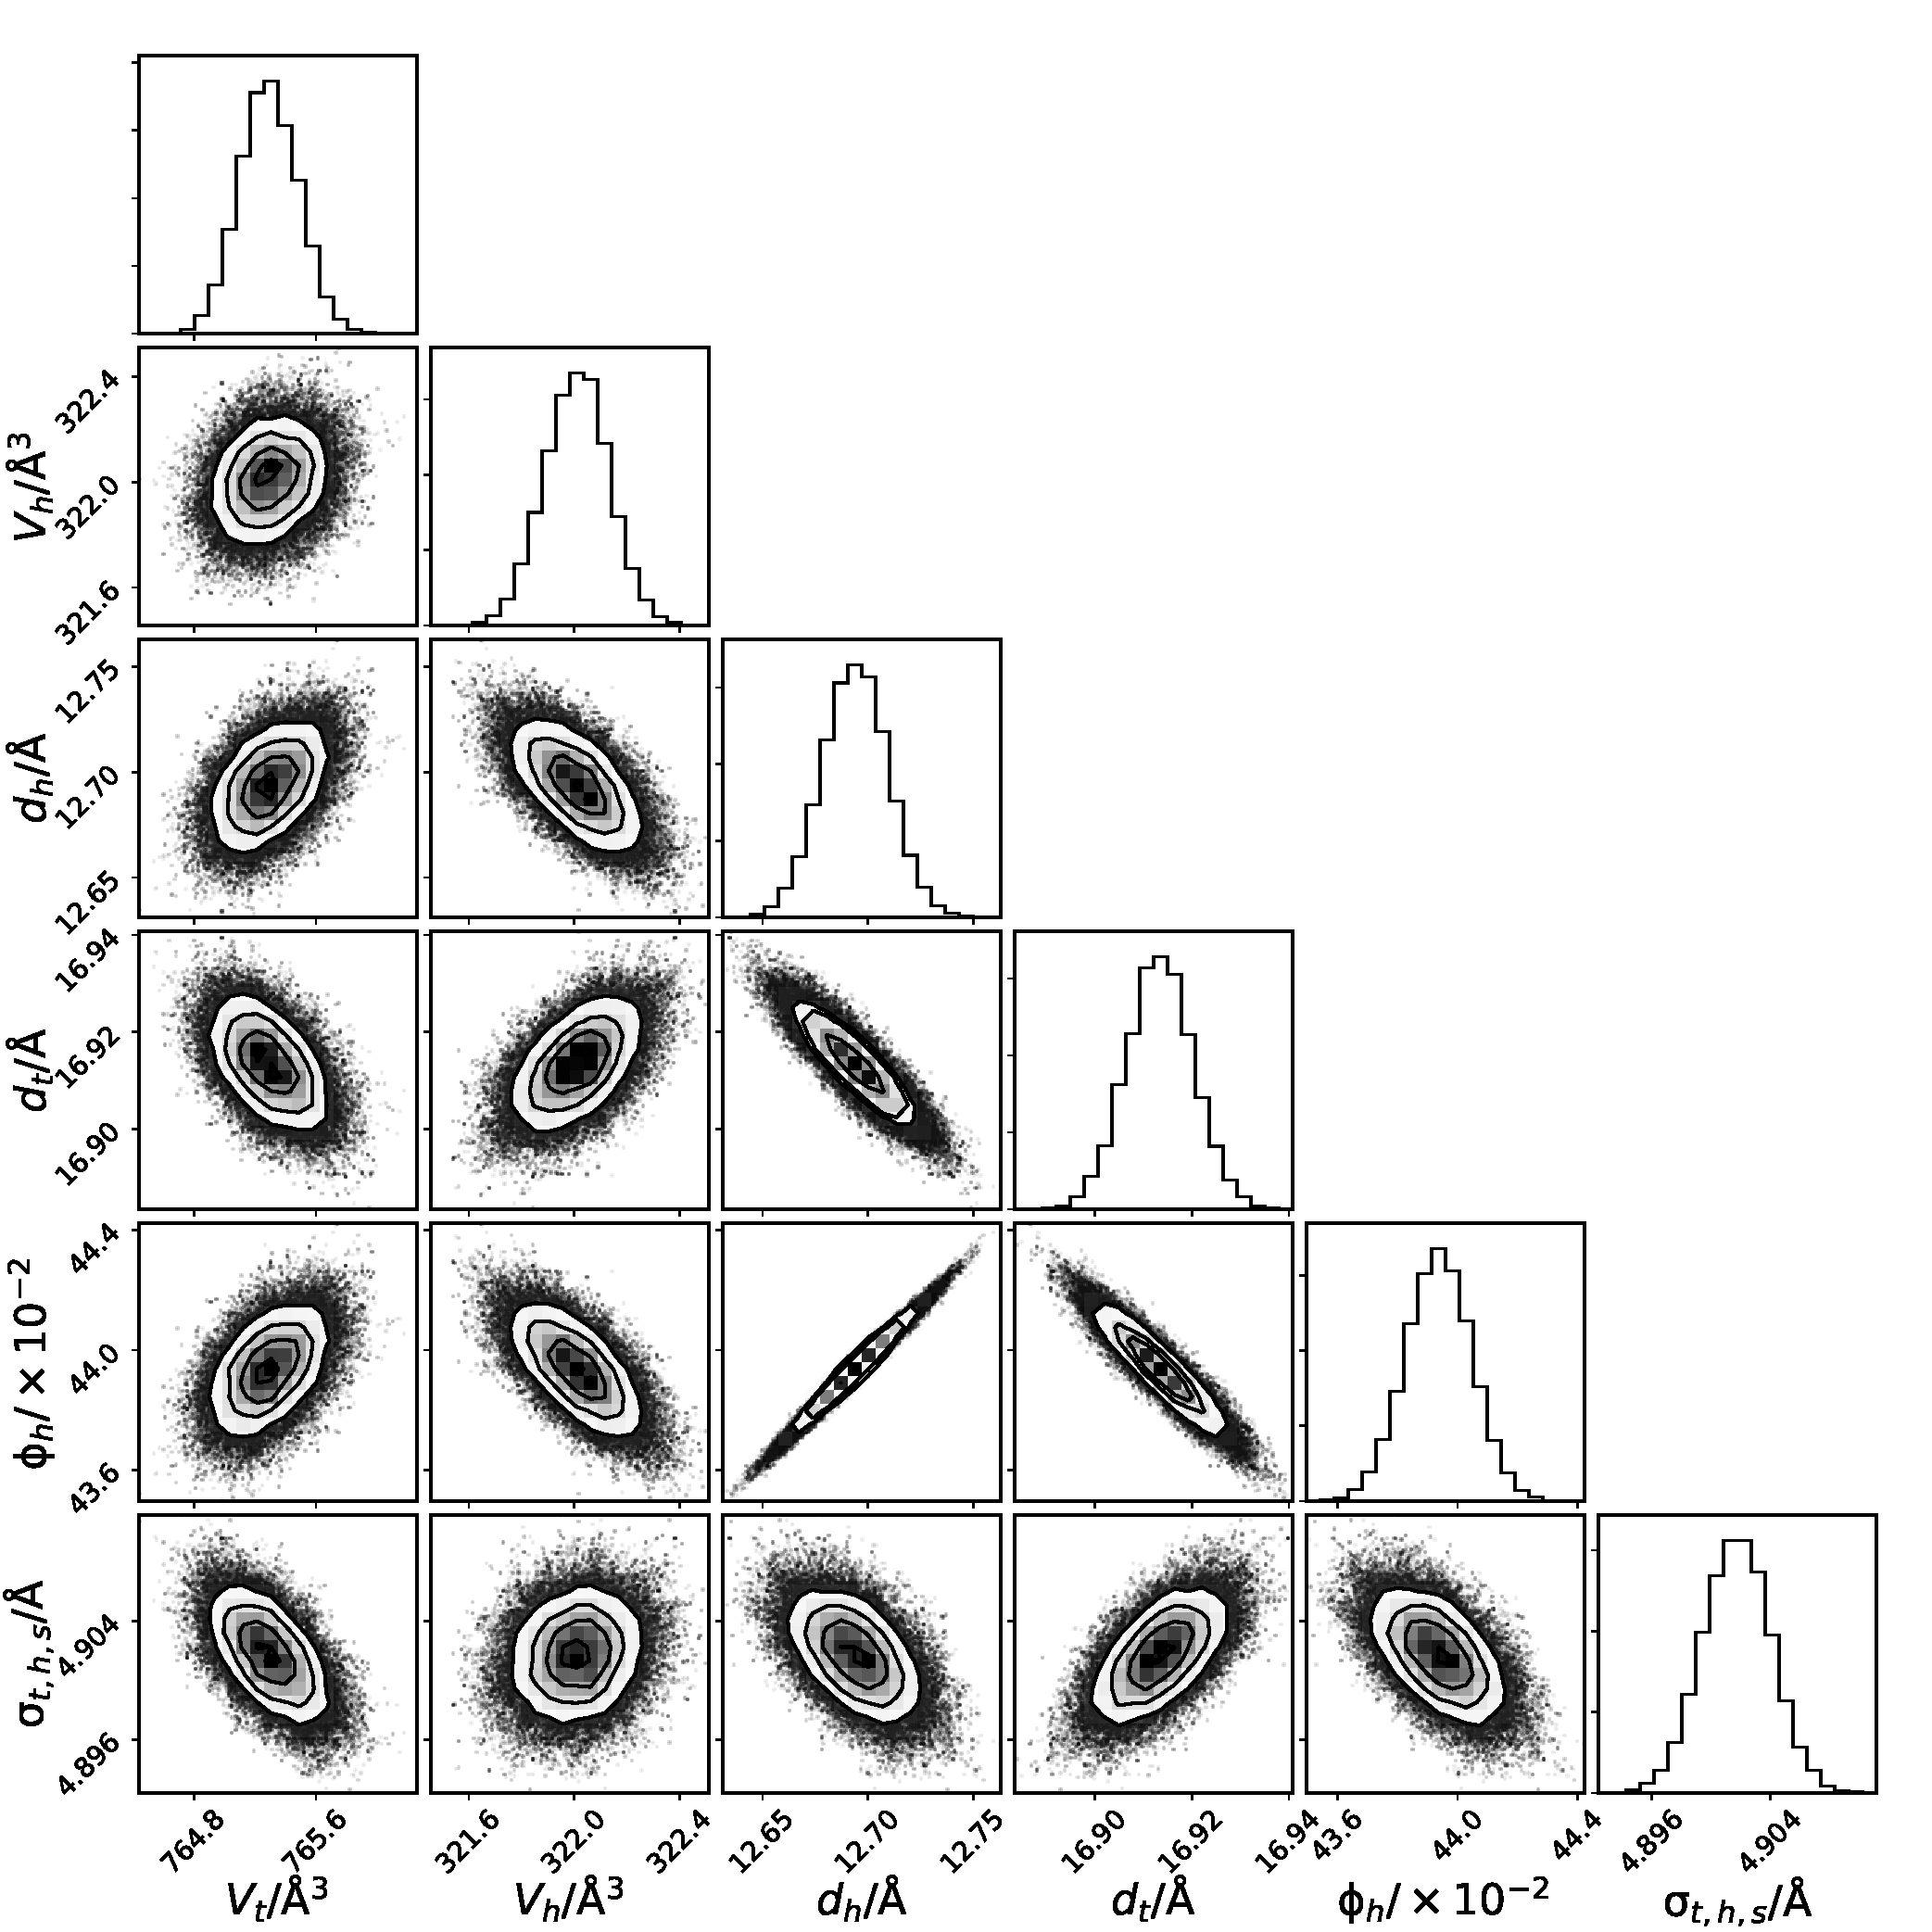
\includegraphics[width=0.50\textwidth]{figures/dppc4_all_corner}
	\caption{The multi-parameter PDFs for the chemically-relevant model of DPPC X-ray reflectometry data at 30 mNm$^{-1}$.}
	\label{fig:dppc5}
\end{figure}
\begin{figure}[H]
	\centering
	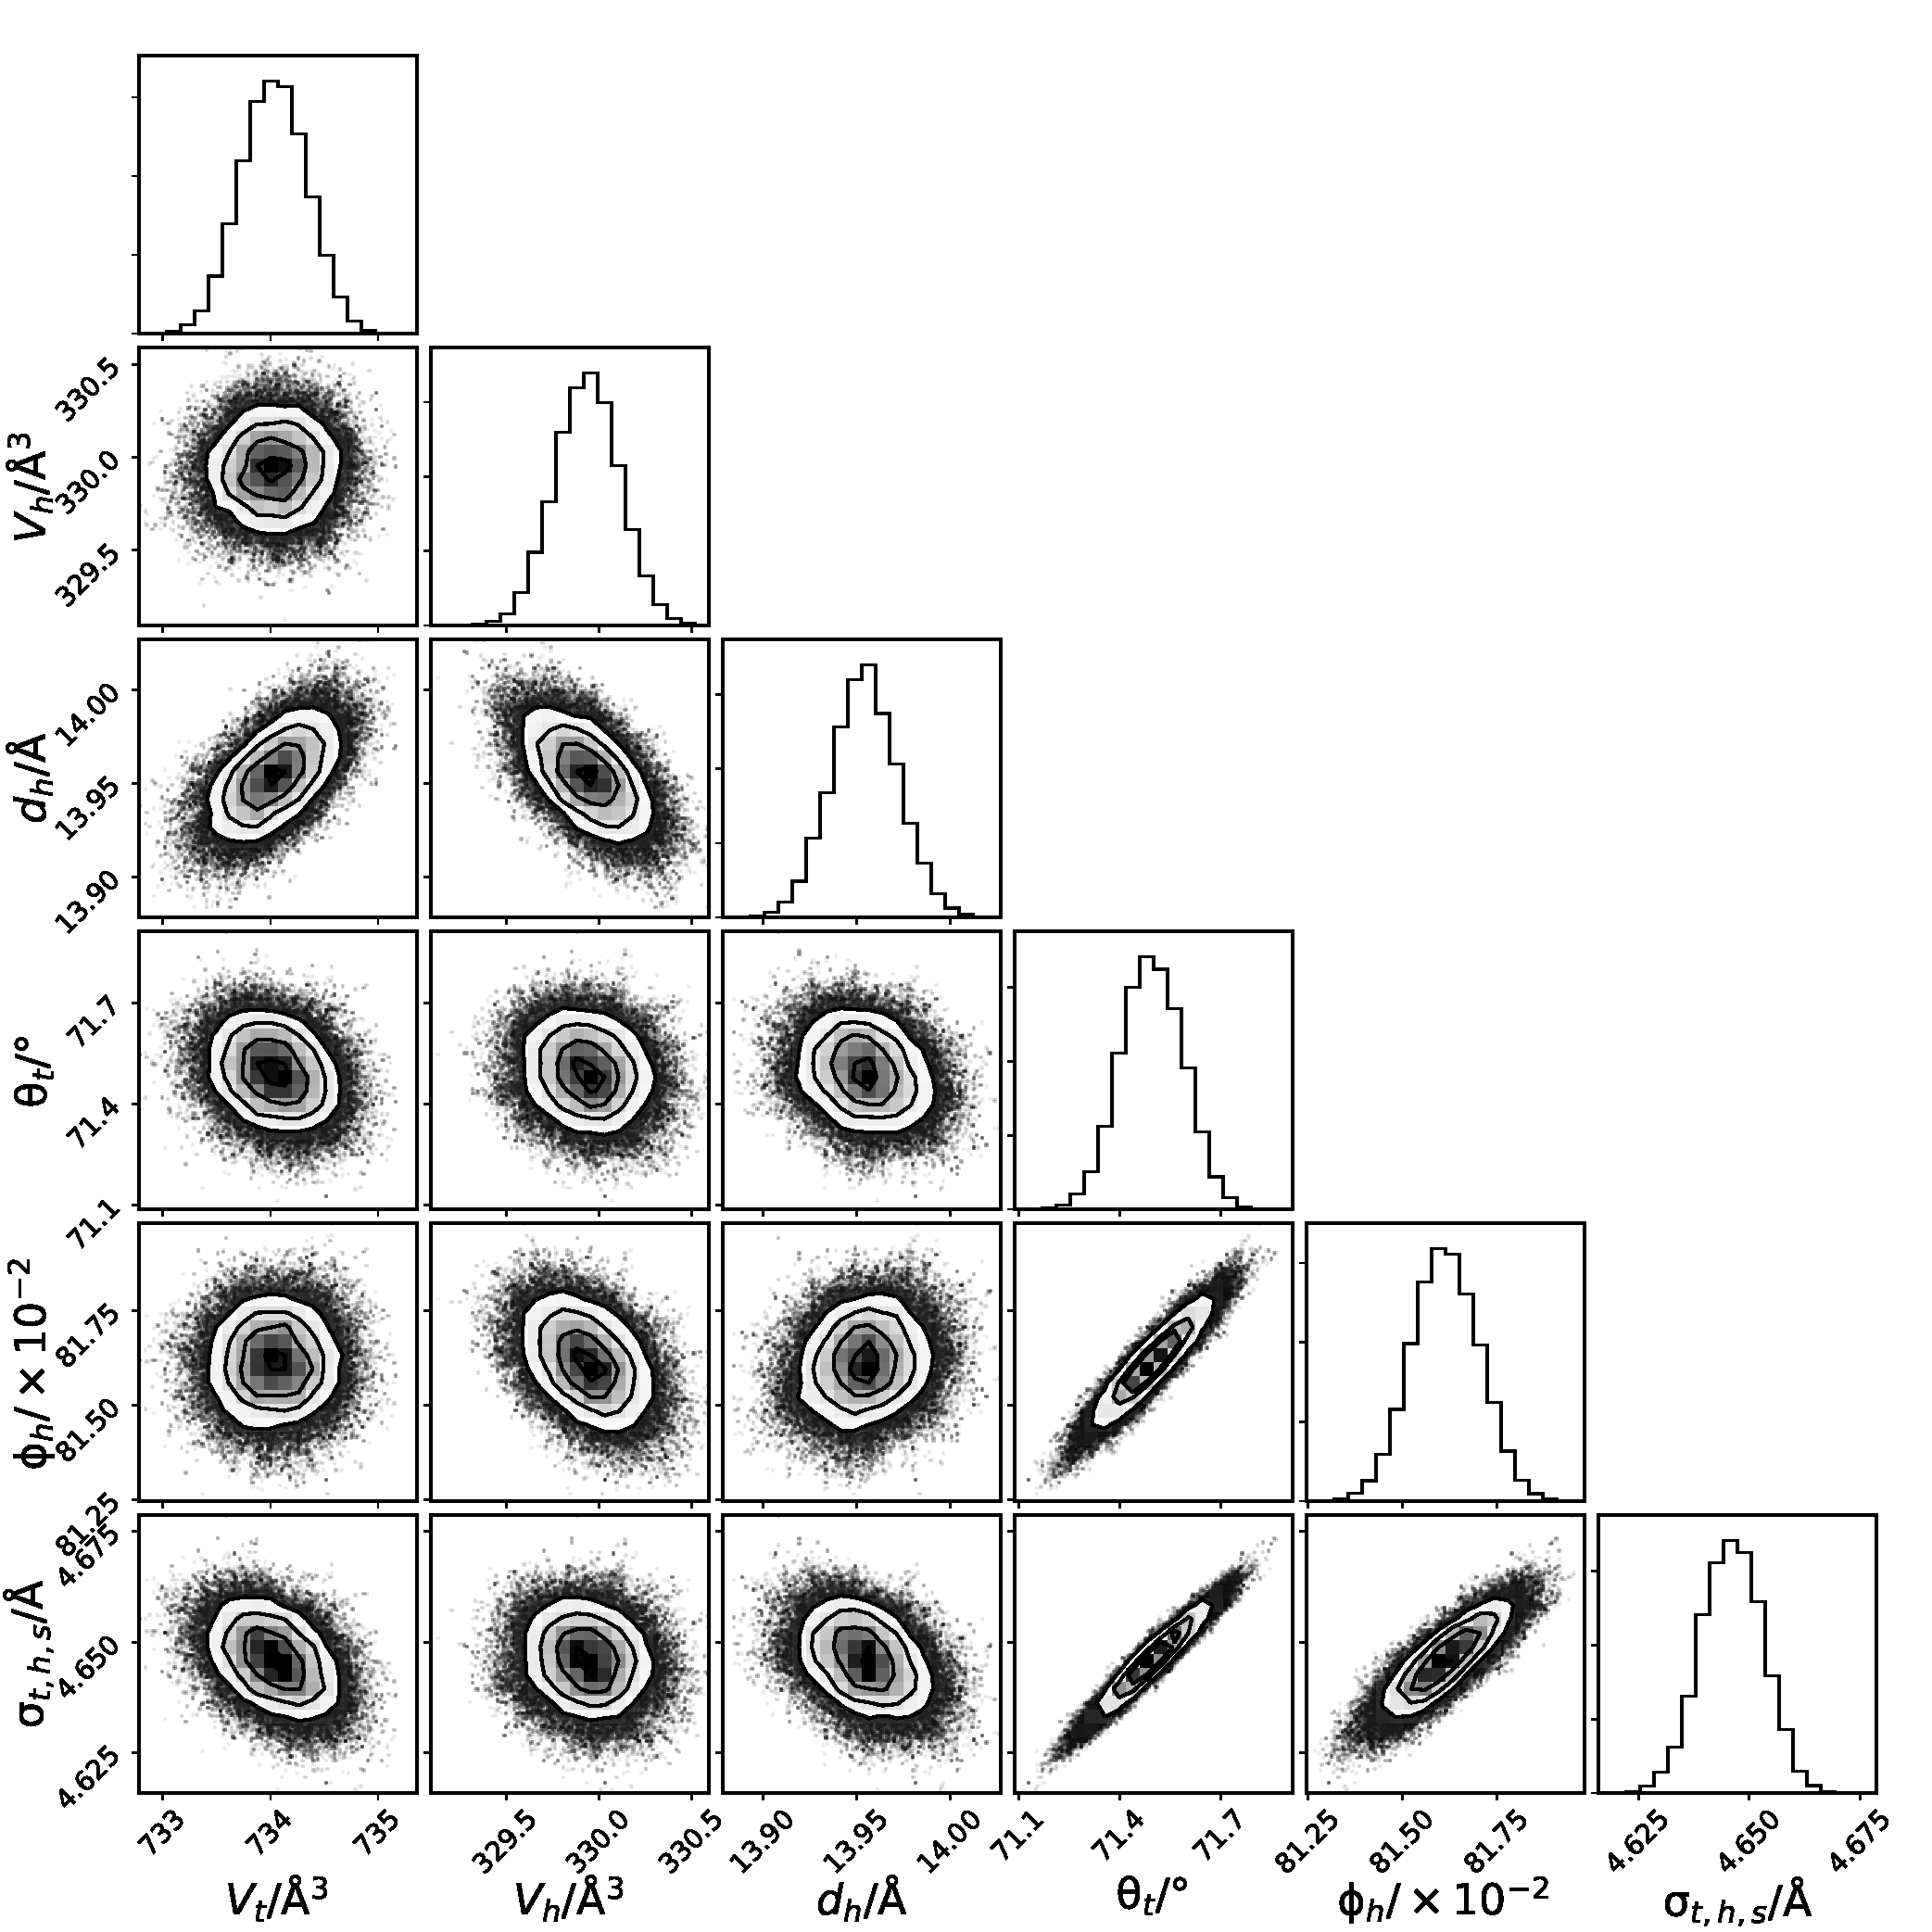
\includegraphics[width=0.50\textwidth]{figures/dmpg1_all_corner}
	\caption{The multi-parameter PDFs for the chemically-relevant model of DMPG X-ray reflectometry data at 15 mNm$^{-1}$.}
	\label{fig:dmpg2}
\end{figure}
\begin{figure}[H]
	\centering
	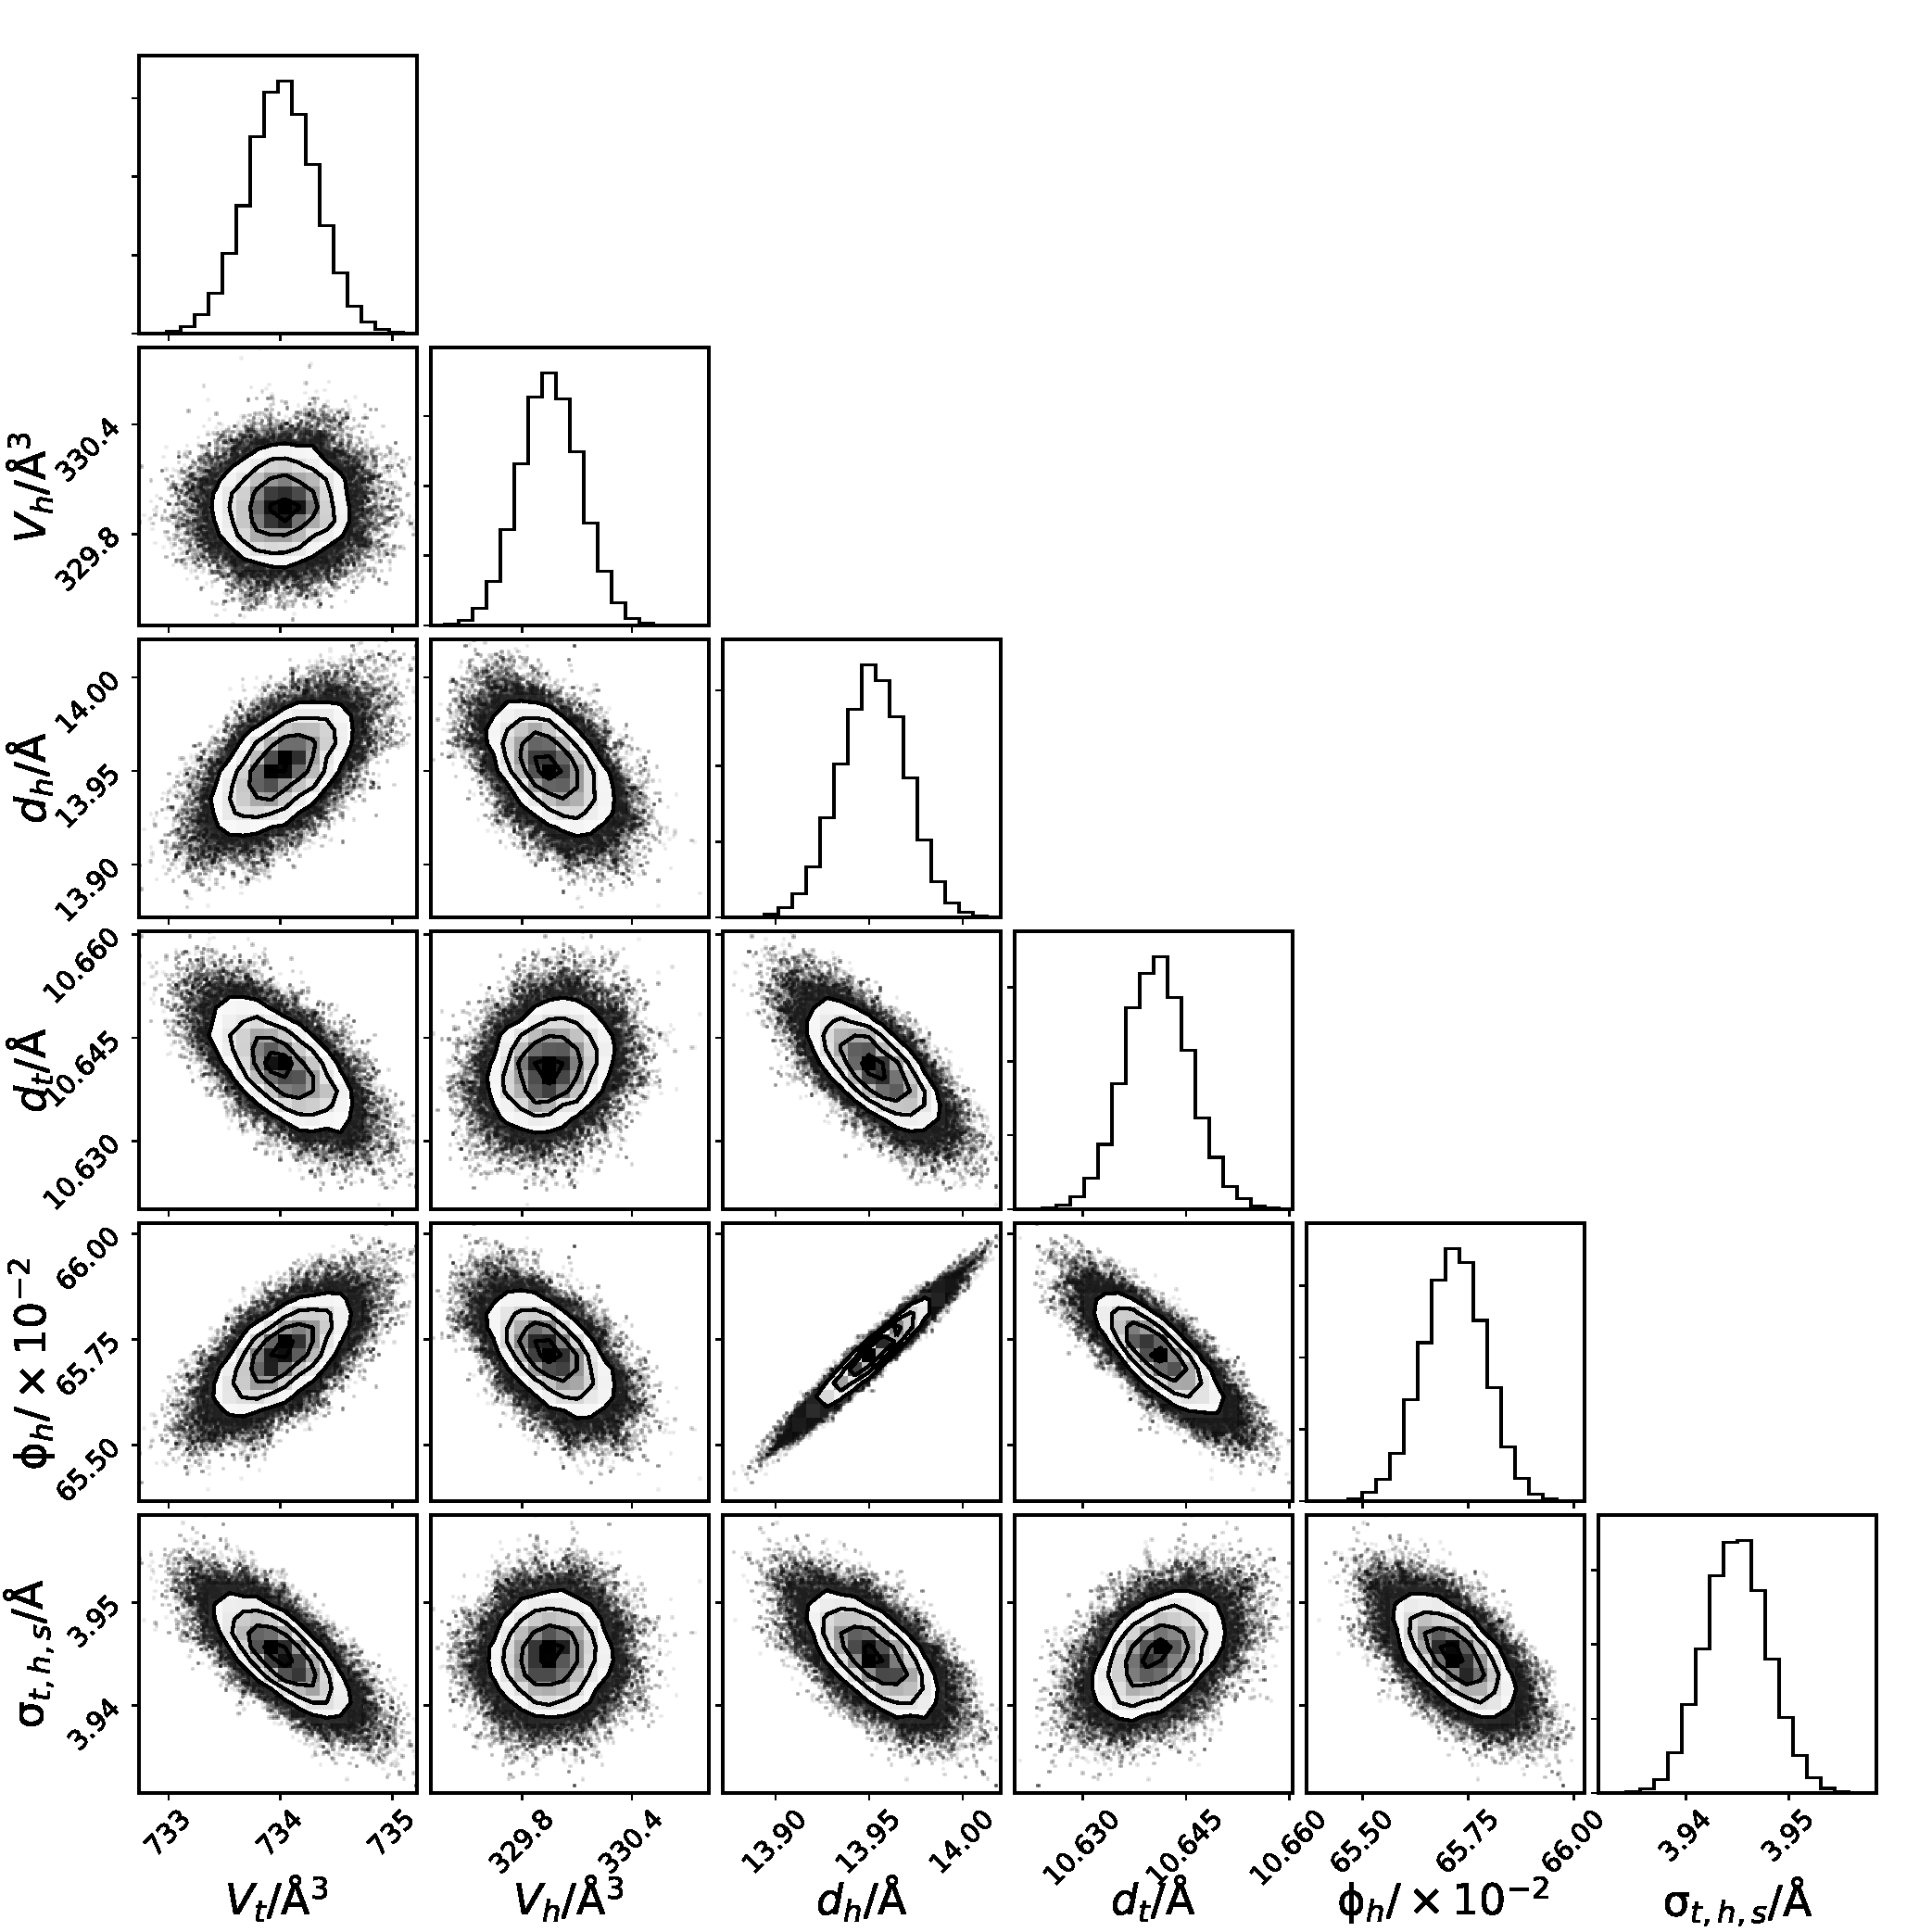
\includegraphics[width=0.50\textwidth]{figures/dmpg2_all_corner}
	\caption{The multi-parameter PDFs for the chemically-relevant model of DMPG X-ray reflectometry data at 20 mNm$^{-1}$. }
	\label{fig:dmpg3}
\end{figure}
\begin{figure}[H]
	\centering
	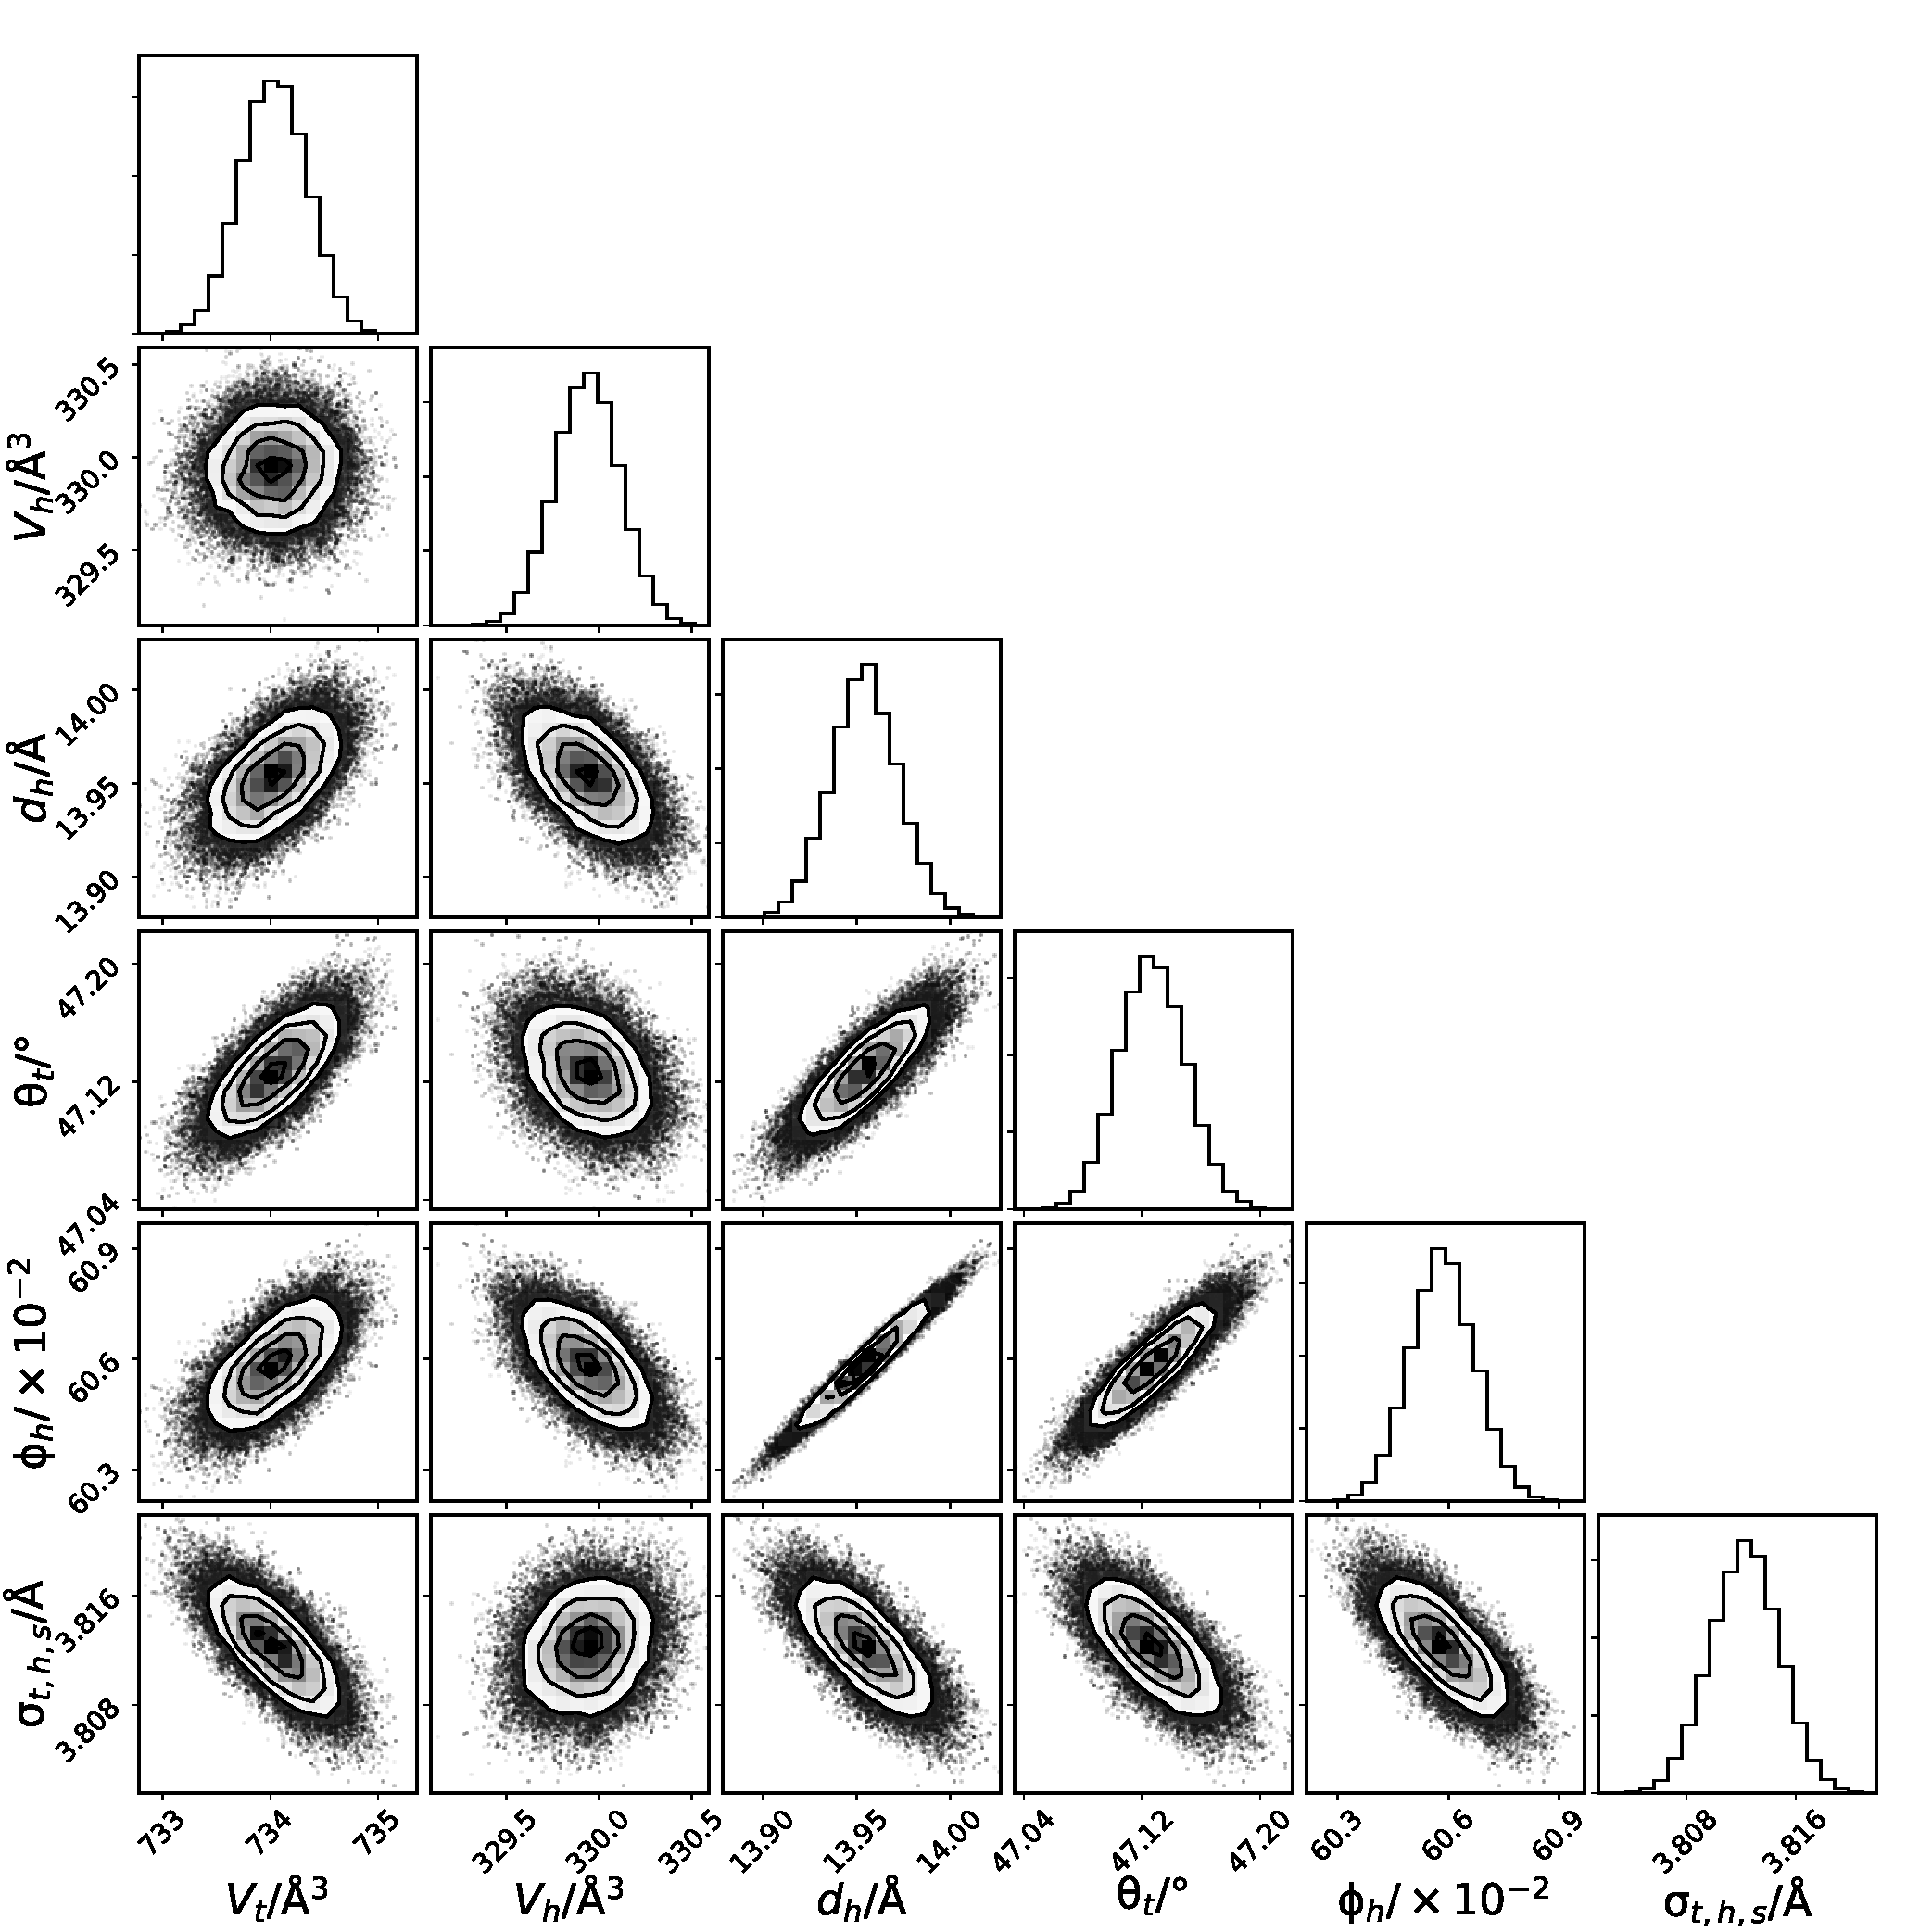
\includegraphics[width=0.50\textwidth]{figures/dmpg3_all_corner}
	\caption{The multi-parameter PDFs for the chemically-relevant model of DMPG X-ray reflectometry data at 25 mNm$^{-1}$.}
	\label{fig:dmpg4}
\end{figure}
\begin{figure}[H]
	\centering
	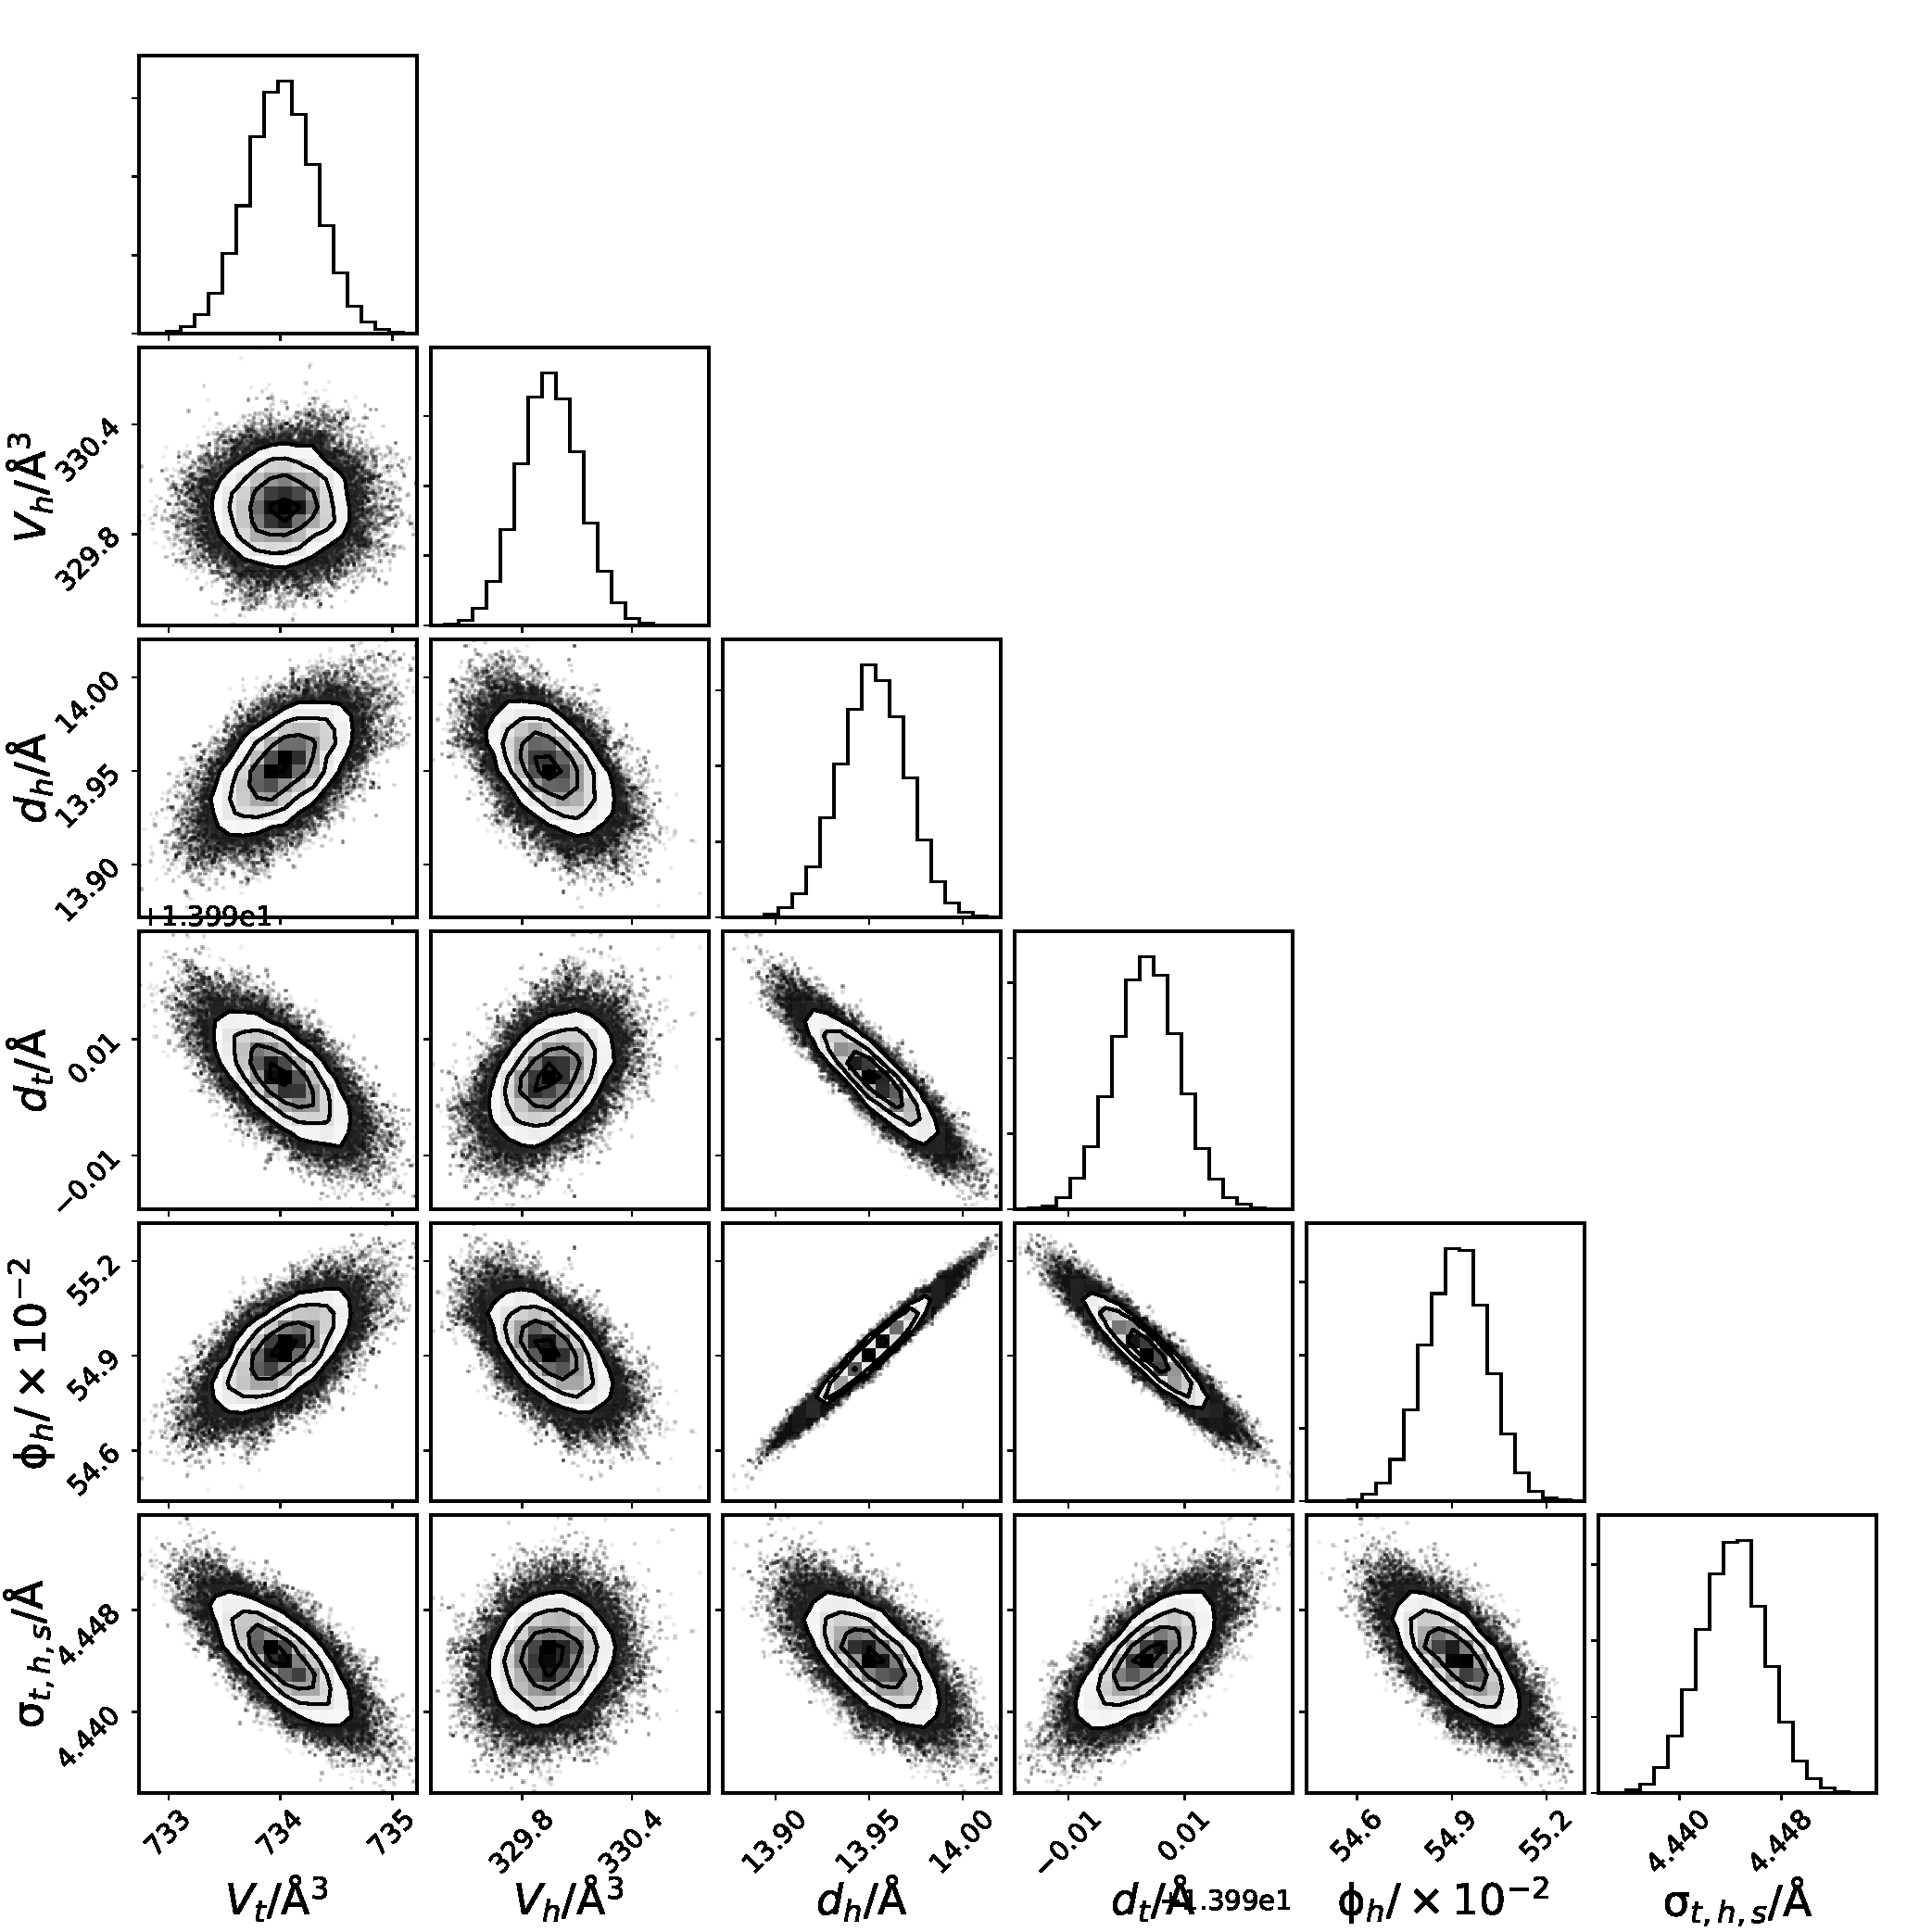
\includegraphics[width=0.50\textwidth]{figures/dmpg4_all_corner}
	\caption{The multi-parameter PDFs for the chemically-relevant model of DMPG X-ray reflectometry data at 30 mNm$^{-1}$.}
	\label{fig:dmpg5}
\end{figure}
\begin{figure}[H]
	\centering
	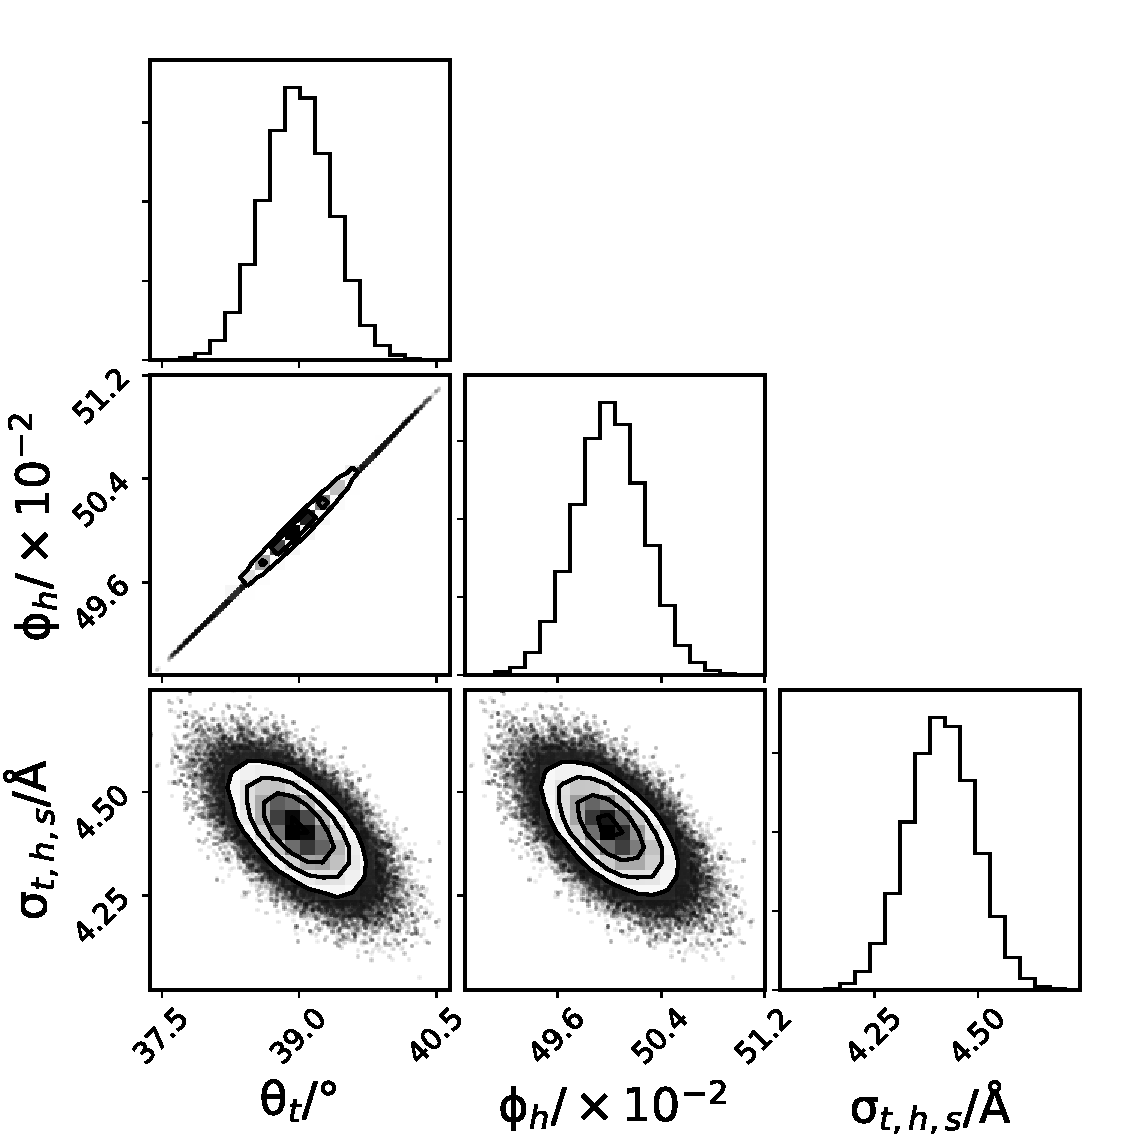
\includegraphics[width=0.50\textwidth]{figures/dmpc_20n_all_corner}
	\caption{The multi-parameter PDFs for the chemically-relevant model of two contrast DMPC neutron reflectometry data at 20 mNm$^{-1}$.}
	\label{fig:dmpcn1}
\end{figure}
\begin{figure}[H]
	\centering
	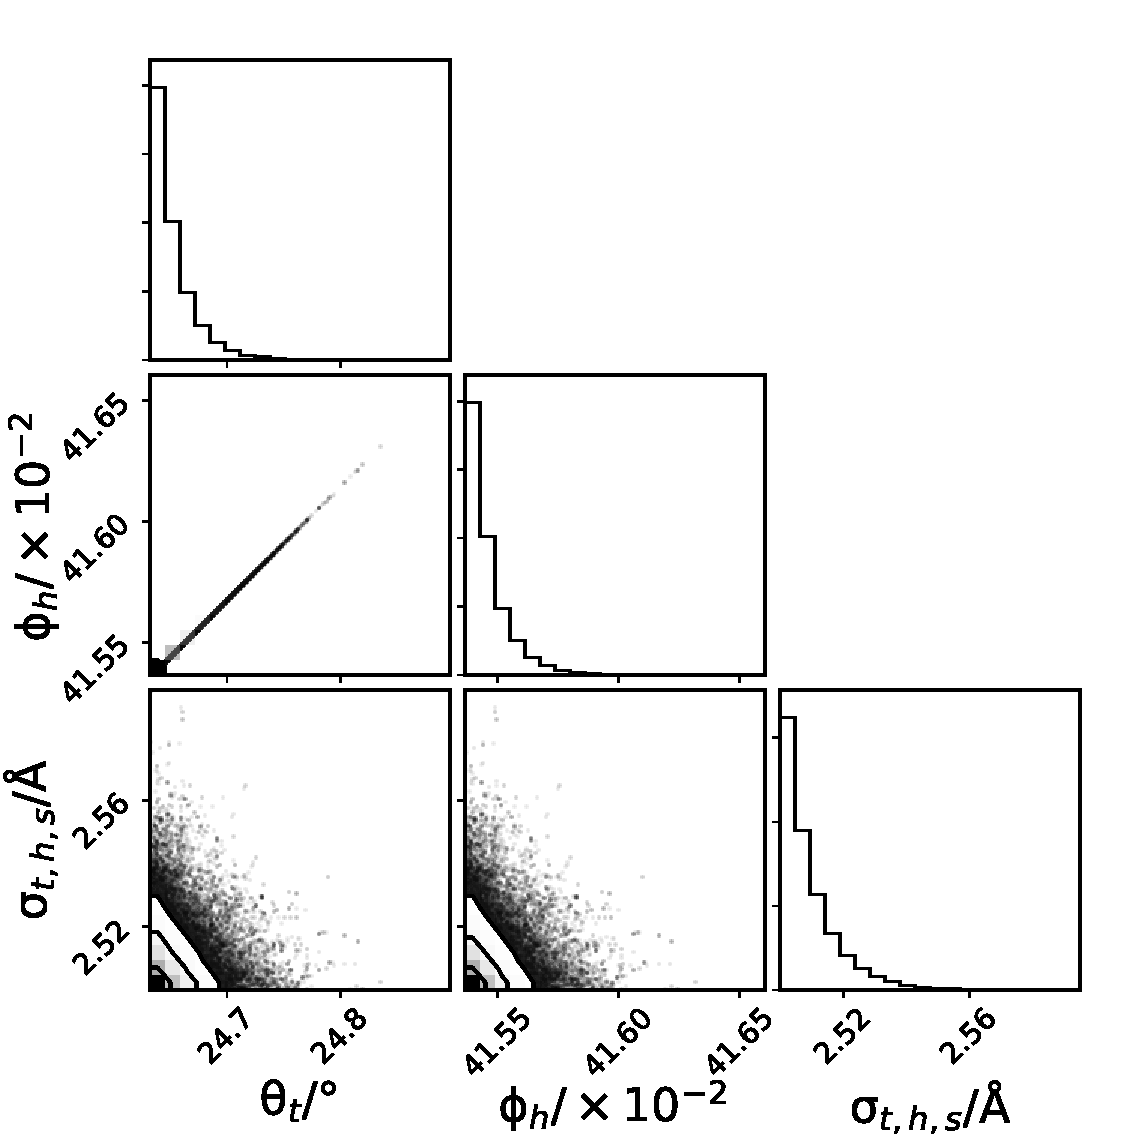
\includegraphics[width=0.50\textwidth]{figures/dmpc_25n_all_corner}
	\caption{The multi-parameter PDFs for the chemically-relevant model of two contrast DMPC neutron reflectometry data at 25 mNm$^{-1}$.}
	\label{fig:dmpcn2}
\end{figure}
\begin{figure}[H]
	\centering
	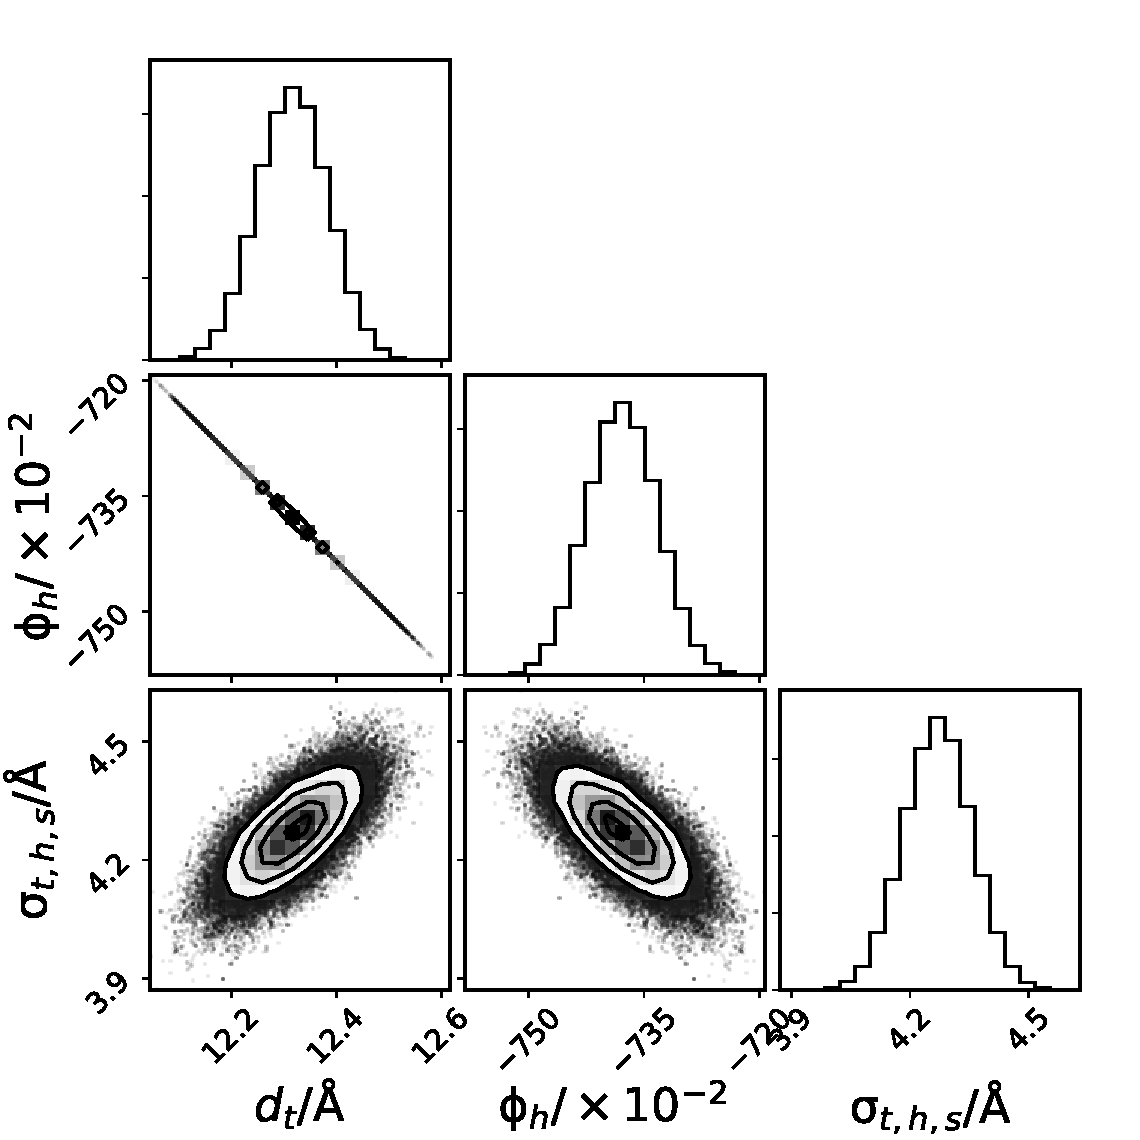
\includegraphics[width=0.50\textwidth]{figures/dppc_15n_all_corner}
	\caption{The multi-parameter PDFs for the chemically-relevant model of two contrast DPPC neutron reflectometry data at 15 mNm$^{-1}$.}
	\label{fig:dppcn1}
\end{figure}
\begin{figure}[H]
	\centering
	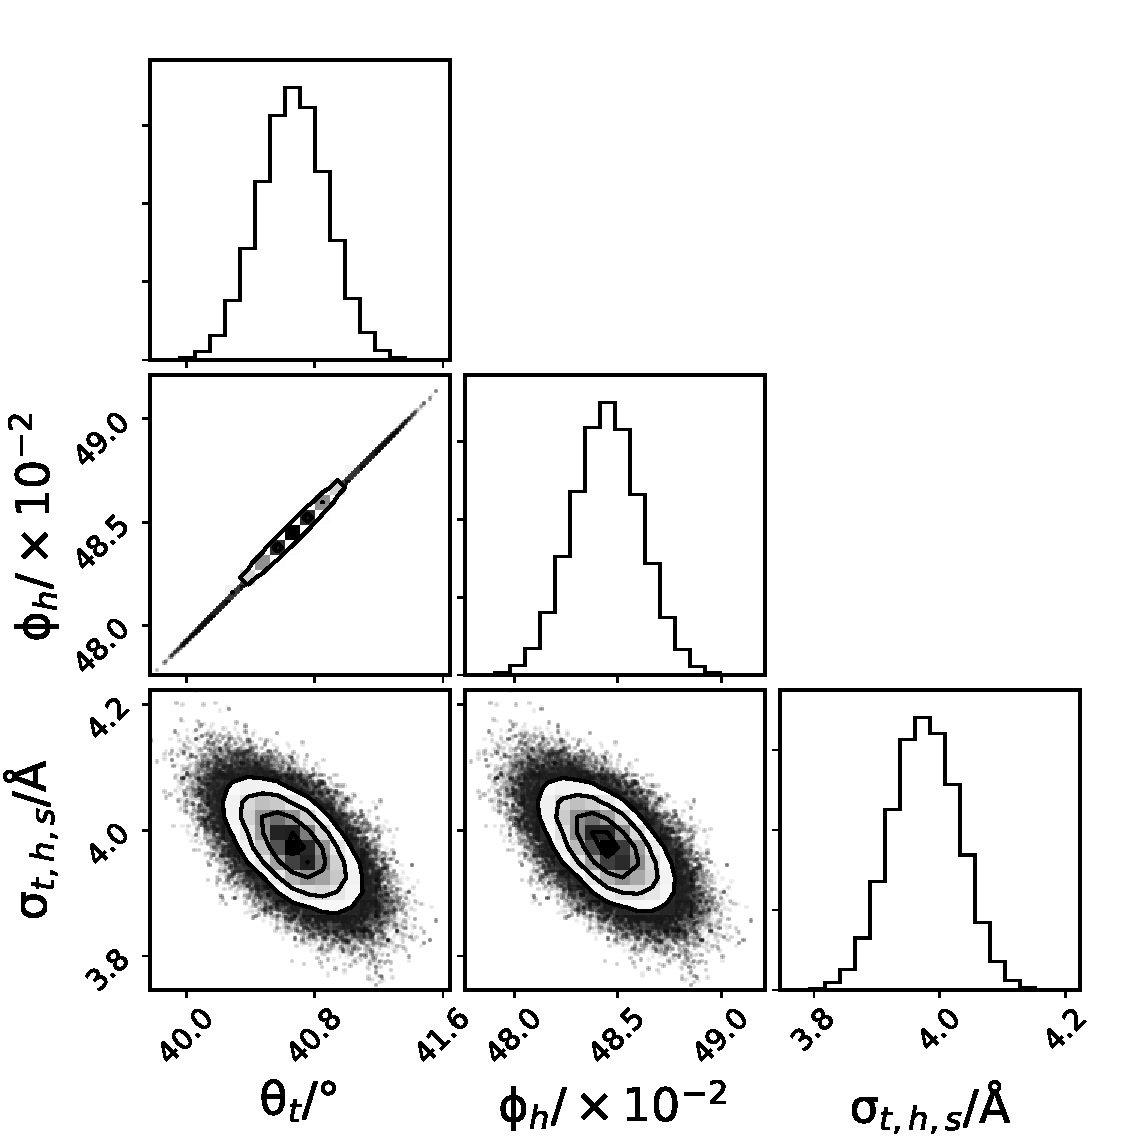
\includegraphics[width=0.50\textwidth]{figures/dppc_20n_all_corner}
	\caption{The multi-parameter PDFs for the chemically-relevant model of two contrast DMPC neutron reflectometry data at 20 mNm$^{-1}$.}
	\label{fig:dppcn2}
\end{figure}

%%%REFERENCES%%%
\bibliography{bibi} %You need to replace "rsc" on this line with the name of your .bib file
\bibliographystyle{rsc} %the RSC's .bst file
\end{document}
